%% Template for Master thesis
%% ===========================
%%
%% You need at least KomaScript v3.0.0,
%% e.g. available in Texlive 2009
\documentclass  [
  paper    = a4,
  BCOR     = 10mm,
  twoside,
  openright,
  fontsize = 12pt,
  fleqn,
  toc      = bibnumbered,
  toc      = listofnumbered,
  numbers  = noendperiod,
  headings = normal,
  listof   = leveldown,
  version  = 3.03
]                                       {scrreprt}

% used pagages
\usepackage     [utf8]                  {inputenc}
\usepackage     [T1]                    {fontenc}
\usepackage                             {color}
\usepackage                             {amssymb}
\usepackage                             {amsmath}
\usepackage                             {graphicx}
\usepackage     [english]               {babel}
\usepackage[square, comma, sort&compress]{natbib}
\usepackage                             {mciteplus}
\usepackage                             {hyperref}

% links
\definecolor{darkblue}{rgb}{0.0,0.0,0.4}
\definecolor{darkgreen}{rgb}{0.0,0.4,0.0}
\hypersetup{
    colorlinks,
    linkcolor=black,
    citecolor=darkgreen,
    urlcolor=darkblue
}

% eigene Pakete

% die folgenden Pakete werden benötigt, um die LHCb-Symbole verwenden zu können.
\usepackage{ifthen} 
\newboolean{articletitles}
\setboolean{articletitles}{true} % False removes titles in references
\newboolean{uprightparticles}
\setboolean{uprightparticles}{false} %Set true for upright particle symbols
\newboolean{inbibliography}
\setboolean{inbibliography}{false} %True once you enter the bibliography
\usepackage{xspace} 
\usepackage{upgreek}
% Ende der benötigten Pakete
\usepackage[scientific-notation=true,
            use-xspace,
            separate-uncertainty]      {siunitx}
\usepackage                            {multirow}
\usepackage                            {array}   
\usepackage                            {esdiff}   

% eigene Einstellungen
\graphicspath{{../figures/}{../figures/detector/}{../figures/analysis/}{../figures/external/}}

% eigene Befehle etc.
\include{lhcb-symbols-def}
% decay channels
\newcommand{\LbDpmunu}{\decay{\Lb}{\Dz\proton\mun\neumb}}
\newcommand{\LbLcmunu}{\decay{\Lb}{\Lc\mun\neumb}}
\newcommand{\LbToDpmunu}{\decay{\Lb}{\Dz\proton\mun\neumb}}
\newcommand{\LbToLcmunu}{\decay{\Lb}{\Lc\mun\neumb}}
\newcommand{\LbToDpmunuX}{\decay{\Lb}{\Dz\proton\mun\neumb X}}
\newcommand{\LbToLcmunuX}{\decay{\Lb}{\Lc\mun\neumb X}}
\newcommand{\LcTopKpi}{\decay{\Lc}{\proton\Km\pip}}
\newcommand{\DToKpi}{\decay{\Dz}{\Km\pip}}

% efficiencies
\newcommand{\effDp}{\ensuremath{\epsilon_{\Dz\proton}}\xspace}
\newcommand{\effLc}{\ensuremath{\epsilon_{\Lc}}\xspace}
\newcommand{\effSel}{\ensuremath{\epsilon_{\text{sel}}}\xspace}
\newcommand{\effSelLc}{\ensuremath{\epsilon_{\text{sel,}\Lc}}\xspace}
\newcommand{\effSelDp}{\ensuremath{\epsilon_{\text{sel,}\Dz\proton}}\xspace}
\newcommand{\effRatio}{\ensuremath{\frac{\effLc}{\effDp}}\xspace}
\newcommand{\effGen}{\ensuremath{\epsilon_{\text{gen}}}\xspace}
\newcommand{\effGenLc}{\ensuremath{\epsilon_{\text{gen,}\Lc}}\xspace}
\newcommand{\effGenDp}{\ensuremath{\epsilon_{\text{gen,}\Dz\proton}}\xspace}
\newcommand{\effPID}[2] {\ensuremath{\epsilon_{{#1}\rightarrow{#2}}}\xspace}    

% measured quantities
\newcommand{\R}{\ensuremath{\mathcal{R}}\xspace}
\newcommand{\asld}{\ensuremath{a_{sl}^d}\xspace}
\newcommand{\MDp}{\ensuremath{M(\Dz\proton)}\xspace}
\newcommand{\Mtrue}[1]{\ensuremath{M_{\text{true}}({#1})}\xspace}
\newcommand{\logIP}{\ensuremath{\log \chi^2_{\text{IP}}}\xspace}
\newcommand{\weight}[1] {\ensuremath{w_{\text{#1}}}\xspace}
\newcommand{\Systerr}[2] {\ensuremath{\Delta{#1}^{\text{{#2}}}_{\text{syst.}}}\xspace}

% yields
\newcommand{\NDp}{\ensuremath{N_{\Dz\proton}}\xspace}
\newcommand{\NLc}{\ensuremath{N_{\Lc}}\xspace}
\newcommand{\Ntrue}[1]{\ensuremath{N_{\text{true}}^{#1}}\xspace}
\newcommand{\Ncand}[1]{\ensuremath{N_{\text{cand}}^{#1}}\xspace}
\newcommand{\NBgdDp}{\ensuremath{N^{\rm bgd}_{\Dz\proton}}\xspace}
\newcommand{\NBgdLc}{\ensuremath{N^{\rm bgd}_{\Lc}}\xspace}

% branching ratios
\newcommand{\DBFDp}{\ensuremath{\mathcal{B}(D^0 \to K^-\pi^+)}\xspace}
\newcommand{\DBFLc}{\ensuremath{\mathcal{B}(\Lambda_c \to p^+K^-\pi^+)}\xspace}

% particles and resonances
\newcommand{\LcResI}{\ensuremath{\Lz_\cquark(2880)^+}\xspace}
\newcommand{\LcResII}{\ensuremath{\Lz_\cquark(2940)^+}\xspace}
\newcommand{\LcRes}[1] {\ensuremath{\Lz_\cquark{#1}^{+}}\xspace}    
\newcommand{\pKpi}{\proton\Km\pip}
\newcommand{\Sigmacp} {\ensuremath{\Sigma_\cquark^{+}}\xspace}    
\newcommand{\SigmacpRes}[1] {\ensuremath{\Sigma_\cquark{#1}^{+}}\xspace}    
\newcommand{\SigmabpRes}[1] {\ensuremath{\Sigma_\bquark{#1}^{+}}\xspace}    
\newcommand{\SigmabRes}[1] {\ensuremath{\Sigma_\bquark{#1}}\xspace}  
\newcommand{\Lcstar}{\ensuremath{\Lz_\cquark^{\ast +}}\xspace}    
\newcommand{\LcstarRes}[1] {\ensuremath{\Lz^{\ast}_\cquark{#1}^{+}}\xspace}    
\newcommand{\XicpRes}[1] {\ensuremath{\Xi_\cquark{#1}^{+}}\xspace}    

% Function names
\newcommand{\BfG}{\text{BfG}}
\newcommand{\DBfG}{\text{DBfG}}
\newcommand{\sigmaL}[1]{\ensuremath{\sigma_{\text{L}_{#1}}}}
\newcommand{\sigmaR}[1]{\ensuremath{\sigma_{\text{R}_{#1}}}}
\newcommand{\CB}{\text{CB}}

\newcommand{\PIDNtruepionvalscient}{5.075}
\newcommand{\PIDNtruepionerrscient}{0.076}
\newcommand{\PIDNtruepionsysterrscient}{0}
\newcommand{\PIDNtruepionexpscient}{3}
\newcommand{\PIDNtruepionval}{5075}
\newcommand{\PIDNtruepionerr}{76}
\newcommand{\PIDNtruepionsysterr}{0}
\newcommand{\PIDNtruePregionkaonvalscient}{9.74}
\newcommand{\PIDNtruePregionkaonerrscient}{0.42}
\newcommand{\PIDNtruePregionkaonsysterrscient}{0}
\newcommand{\PIDNtruePregionkaonexpscient}{0}
\newcommand{\PIDNtruePregionkaonval}{10}
\newcommand{\PIDNtruePregionkaonerr}{0}
\newcommand{\PIDNtruePregionkaonsysterr}{0}
\newcommand{\LcResImeanvalscient}{2.88185}
\newcommand{\LcResImeanerrscient}{0.00035}
\newcommand{\LcResImeansysterrscient}{0}
\newcommand{\LcResImeanexpscient}{3}
\newcommand{\LcResImeanval}{2882}
\newcommand{\LcResImeanerr}{0}
\newcommand{\LcResImeansysterr}{0}
\newcommand{\NLcvalscient}{1.5837}
\newcommand{\NLcerrscient}{0.0098}
\newcommand{\NLcsysterrscient}{0}
\newcommand{\NLcexpscient}{6}
\newcommand{\NLcval}{1583700}
\newcommand{\NLcerr}{9800}
\newcommand{\NLcsysterr}{0}
\newcommand{\LcResIIwidthvalscient}{2.62}
\newcommand{\LcResIIwidtherrscient}{0.79}
\newcommand{\LcResIIwidthsysterrscient}{0}
\newcommand{\LcResIIwidthexpscient}{1}
\newcommand{\LcResIIwidthval}{26}
\newcommand{\LcResIIwidtherr}{8}
\newcommand{\LcResIIwidthsysterr}{0}
\newcommand{\NDpresIIIvalscient}{2.38}
\newcommand{\NDpresIIIerrscient}{0.44}
\newcommand{\NDpresIIIsysterrscient}{0}
\newcommand{\NDpresIIIexpscient}{3}
\newcommand{\NDpresIIIval}{2380}
\newcommand{\NDpresIIIerr}{440}
\newcommand{\NDpresIIIsysterr}{0}
\newcommand{\effLcval}{0.0014}
\newcommand{\effLcerr}{0.0001}
\newcommand{\effLcsysterr}{0.0000}
\newcommand{\BRLcTopKpival}{0.07}
\newcommand{\BRLcTopKpierr}{0.00}
\newcommand{\BRLcTopKpisysterr}{0.00}
\newcommand{\effSelDpval}{0.005}
\newcommand{\effSelDperr}{0.000}
\newcommand{\effSelDpsysterr}{0.000}
\newcommand{\misIDratiovalscient}{698.0}
\newcommand{\misIDratioerrscient}{24.0}
\newcommand{\misIDratiosysterrscient}{0.0}
\newcommand{\misIDratioexpscient}{-2}
\newcommand{\misIDratioval}{7}
\newcommand{\misIDratioerr}{0}
\newcommand{\misIDratiosysterr}{0}
\newcommand{\effDpval}{0.001}
\newcommand{\effDperr}{0.000}
\newcommand{\effDpsysterr}{0.000}
\newcommand{\NDpresIvalscient}{1.35}
\newcommand{\NDpresIerrscient}{0.15}
\newcommand{\NDpresIsysterrscient}{0}
\newcommand{\NDpresIexpscient}{3}
\newcommand{\NDpresIval}{1350}
\newcommand{\NDpresIerr}{150}
\newcommand{\NDpresIsysterr}{0}
\newcommand{\PIDNcandkaonvalscient}{2.175}
\newcommand{\PIDNcandkaonerrscient}{0.047}
\newcommand{\PIDNcandkaonsysterrscient}{0}
\newcommand{\PIDNcandkaonexpscient}{3}
\newcommand{\PIDNcandkaonval}{2175}
\newcommand{\PIDNcandkaonerr}{47}
\newcommand{\PIDNcandkaonsysterr}{0}
\newcommand{\effGenLcval}{0.3}
\newcommand{\effGenLcerr}{0.0}
\newcommand{\effGenLcsysterr}{0.0}
\newcommand{\effGenDpval}{0.2}
\newcommand{\effGenDperr}{0.1}
\newcommand{\effGenDpsysterr}{0.0}
\newcommand{\effRatiovalscient}{1.22}
\newcommand{\effRatioerrscient}{0.32}
\newcommand{\effRatiosysterrscient}{0}
\newcommand{\effRatioexpscient}{0}
\newcommand{\effRatioval}{1}
\newcommand{\effRatioerr}{0}
\newcommand{\effRatiosysterr}{0}
\newcommand{\misIDratiobinIvalscient}{380.0}
\newcommand{\misIDratiobinIerrscient}{23.0}
\newcommand{\misIDratiobinIsysterrscient}{0.0}
\newcommand{\misIDratiobinIexpscient}{-2}
\newcommand{\misIDratiobinIval}{4}
\newcommand{\misIDratiobinIerr}{0}
\newcommand{\misIDratiobinIsysterr}{0}
\newcommand{\NDpbkgvalscient}{9.42}
\newcommand{\NDpbkgerrscient}{0.14}
\newcommand{\NDpbkgsysterrscient}{0}
\newcommand{\NDpbkgexpscient}{3}
\newcommand{\NDpbkgval}{9420}
\newcommand{\NDpbkgerr}{140}
\newcommand{\NDpbkgsysterr}{0}
\newcommand{\effSelLcval}{0.0039}
\newcommand{\effSelLcerr}{0.0000}
\newcommand{\effSelLcsysterr}{0.0000}
\newcommand{\Rval}{0.03}
\newcommand{\Rerr}{0.01}
\newcommand{\Rsysterr}{0.00}
\newcommand{\PIDNtruekaonvalscient}{1.26}
\newcommand{\PIDNtruekaonerrscient}{0.055}
\newcommand{\PIDNtruekaonsysterrscient}{0}
\newcommand{\PIDNtruekaonexpscient}{3}
\newcommand{\PIDNtruekaonval}{1260}
\newcommand{\PIDNtruekaonerr}{55}
\newcommand{\PIDNtruekaonsysterr}{0}
\newcommand{\LcResIImeanvalscient}{2.9368}
\newcommand{\LcResIImeanerrscient}{0.0021}
\newcommand{\LcResIImeansysterrscient}{0}
\newcommand{\LcResIImeanexpscient}{3}
\newcommand{\LcResIImeanval}{2937}
\newcommand{\LcResIImeanerr}{2}
\newcommand{\LcResIImeansysterr}{0}
\newcommand{\BRDToKpival}{0.039}
\newcommand{\BRDToKpierr}{0.000}
\newcommand{\BRDToKpisysterr}{0.001}
\newcommand{\PIDNtrueprotonvalscient}{1.88}
\newcommand{\PIDNtrueprotonerrscient}{0.065}
\newcommand{\PIDNtrueprotonsysterrscient}{0}
\newcommand{\PIDNtrueprotonexpscient}{3}
\newcommand{\PIDNtrueprotonval}{1880}
\newcommand{\PIDNtrueprotonerr}{65}
\newcommand{\PIDNtrueprotonsysterr}{0}
\newcommand{\LcResIwidthvalscient}{8.9}
\newcommand{\LcResIwidtherrscient}{1.4}
\newcommand{\LcResIwidthsysterrscient}{0}
\newcommand{\LcResIwidthexpscient}{0}
\newcommand{\LcResIwidthval}{9}
\newcommand{\LcResIwidtherr}{1}
\newcommand{\LcResIwidthsysterr}{0}
\newcommand{\PIDNcandprotonvalscient}{9.89}
\newcommand{\PIDNcandprotonerrscient}{0.31}
\newcommand{\PIDNcandprotonsysterrscient}{0}
\newcommand{\PIDNcandprotonexpscient}{2}
\newcommand{\PIDNcandprotonval}{989}
\newcommand{\PIDNcandprotonerr}{31}
\newcommand{\PIDNcandprotonsysterr}{0}
\newcommand{\NDpcontvalscient}{1.808}
\newcommand{\NDpconterrscient}{0.067}
\newcommand{\NDpcontsysterrscient}{0}
\newcommand{\NDpcontexpscient}{4}
\newcommand{\NDpcontval}{18080}
\newcommand{\NDpconterr}{670}
\newcommand{\NDpcontsysterr}{0}
\newcommand{\misIDratiobinIIvalscient}{625.0}
\newcommand{\misIDratiobinIIerrscient}{36.0}
\newcommand{\misIDratiobinIIsysterrscient}{0.0}
\newcommand{\misIDratiobinIIexpscient}{-2}
\newcommand{\misIDratiobinIIval}{6}
\newcommand{\misIDratiobinIIerr}{0}
\newcommand{\misIDratiobinIIsysterr}{0}
\newcommand{\PIDNcandpionvalscient}{5.052}
\newcommand{\PIDNcandpionerrscient}{0.071}
\newcommand{\PIDNcandpionsysterrscient}{0}
\newcommand{\PIDNcandpionexpscient}{3}
\newcommand{\PIDNcandpionval}{5052}
\newcommand{\PIDNcandpionerr}{71}
\newcommand{\PIDNcandpionsysterr}{0}
\newcommand{\misIDratiobinIIIvalscient}{117.9}
\newcommand{\misIDratiobinIIIerrscient}{7.8}
\newcommand{\misIDratiobinIIIsysterrscient}{0.0}
\newcommand{\misIDratiobinIIIexpscient}{-1}
\newcommand{\misIDratiobinIIIval}{12}
\newcommand{\misIDratiobinIIIerr}{1}
\newcommand{\misIDratiobinIIIsysterr}{0}
\newcommand{\PIDNtruePregionpionvalscient}{5.925}
\newcommand{\PIDNtruePregionpionerrscient}{0.089}
\newcommand{\PIDNtruePregionpionsysterrscient}{0}
\newcommand{\PIDNtruePregionpionexpscient}{1}
\newcommand{\PIDNtruePregionpionval}{59}
\newcommand{\PIDNtruePregionpionerr}{1}
\newcommand{\PIDNtruePregionpionsysterr}{0}
\newcommand{\NDpvalscient}{2.294}
\newcommand{\NDperrscient}{0.085}
\newcommand{\NDpsysterrscient}{0.032}
\newcommand{\NDpexpscient}{4}
\newcommand{\NDpval}{22940}
\newcommand{\NDperr}{850}
\newcommand{\NDpsysterr}{320}
\newcommand{\NDpresIIvalscient}{1.13}
\newcommand{\NDpresIIerrscient}{0.23}
\newcommand{\NDpresIIsysterrscient}{0}
\newcommand{\NDpresIIexpscient}{3}
\newcommand{\NDpresIIval}{1130}
\newcommand{\NDpresIIerr}{230}
\newcommand{\NDpresIIsysterr}{0}
\newcommand{\PIDNtruePregionprotonvalscient}{9.2}
\newcommand{\PIDNtruePregionprotonerrscient}{0.32}
\newcommand{\PIDNtruePregionprotonsysterrscient}{0}
\newcommand{\PIDNtruePregionprotonexpscient}{2}
\newcommand{\PIDNtruePregionprotonval}{920}
\newcommand{\PIDNtruePregionprotonerr}{32}
\newcommand{\PIDNtruePregionprotonsysterr}{0}
\newcommand{\SystNDpfit}{316.0}
\newcommand{\SystNDpfitpercent}{1.38}
\newcommand{\SystNDp}{316.0}


\begin{document}
  %% title pages similar to providet template instead of maketitle
  %\include{titlepages-ger} % select either german
  %% this will generate title pages similar to the template provided
%% by the Department of Physics and Astronomy Heidelberg
%%
%% More information:
%% http://www.physik.uni-heidelberg.de/aktuelles/studium/
%% (PDF link: ...studium/download/145/Vorlage_Diplomarbeit_Formular.pdf)

%% Titleintro
\thispagestyle{empty}
\begin{center}
  \renewcommand{\baselinestretch}{2.00}
  \Large\sffamily
  Department of Physics and Astronomy\\
  \large University of Heidelberg
  \par\vfill\normalfont
  Master thesis\\
  in Physics\\
  submitted by\\
  Patrick Fahner\\
  born in Mannheim\\
  September 2015
\end{center}
\cleardoublepage

%% Titlepage
\thispagestyle{empty}
\begin{center}
  \renewcommand{\baselinestretch}{2.00}
  \Large\bfseries\sffamily
  \boldmath
    Measurement of the branching ratio for the decay \LbToDpmunuX with the \lhcb experiment
  \unboldmath
  \par
  \vfill
  \large\normalfont
  This Master thesis has been carried out by\\
  Patrick Fahner\\
  at the\\
  Physikalisches Institut\\
  under the supervision of\\
  Prof. Dr. Ulrich Uwer\\
  and\\
  Dr. Mika Vesterinen
  %% additionally insert second supervisor here if carrying out an
  %% external diploma thesis. Reduce vspace in L. 44 accordingly.
\end{center}\par
%\vspace{1\baselineskip}

% reset baselinestretch
\renewcommand{\baselinestretch}{1.00}\normalsize
 % or english title page
  \include{abstracts}

  \tableofcontents
  %% Put your contents here
  \chapter{Introduction}
\label{sec:Introduction}
Developed about 40 years ago, the Standard Model of Particle Physics very successfully describes the properties of the known elementary particles and their interactions among each other \cite{SM_Glashow, SM_Salam, SM_Weinberg}.
It includes the electromagnetic, the strong and the weak interaction.
Until today it has been probed with tremendous precision.
With the exception of the neutrino masses, no results contradicting its predictions have been found so far.
With the discovery of the Higgs boson in 2012 \cite{Higgs_ATLAS, Higgs_CMS}, confirming the theory of electroweak symmetry breaking, the success of the Standard Model reached its climax.

Nonetheless, there are still open questions, which the Standard Model does not answer:
Where does the asymmetry between matter and antimatter come from\footnote{Admittedly, with the $\mathcal{CP}$-violation the Standard Model provides a framework for matter-antimatter asymmetry, though it is not sufficient to explain the observed asymmetry in the universe.}?
What is the origin of dark matter and of dark energy, making up about 95\% of our universe in total \cite{Planck_Universe}?
How can gravitation be formulated as a quantum field theory and be combined with the Standard Model interaction to a more general theory of forces?

The Large Hadron Collider (LHC) of the European Organization for Nuclear Research (CERN) at Geneva, Switzerland is ``the world's largest and most powerful particle accelerator" \cite{CERN_LHC_web} dedicated to tackle those questions.
One of the four big experiments located at the LHC is the \lhcb-experiment.
It is built to probe the Standard Model to a high precision and to find indirect evidence for physics beyond the Standard Model, often referred to as ``New Physics (NP)", by the study of hadron decays containing a \bquark- or \cquark-quark.
These hadrons provide an excellent laboratory for the measurement of observables sensitive to New Physics like $\mathcal{CP}$-violation and many more.
It allows furthermore to do spectroscopical analyses with bound heavy quark states leading to a better understanding of Quantum Chromodynamics (QCD), the theory of the strong interaction responsible for the bindings of quarks to hadrons.
Unfortunately, QCD cannot be treated perturbatively in the energy regime of hadrons.
Thus, theoretical predictions of such \bquark-/\cquark-hadron decays are always forced to make use of approximations, for instance of the Heavy Quark Effective Theory (HQET) \cite{HQET_Introduction}.
The quark model of such theories predicts plenty of \bquark-/\cquark-hadron resonances \cite{cBaryons_Predictions}.
Consequently, the more resonances and particles including their properties are measured, the better these effective theories can be adjusted and the better gets the knowledge of the strong interaction.
While the \B factories and hadron colliders made a great progress in studying \bquark mesons, the knowledge of \bquark baryons is rather poor.

This thesis aims to measure the branching fraction of the semileptonic decay \LbToDpmunuX in the form of a relative branching fraction ratio 
\begin{align*}
    \R := \frac{\BR(\LbToDpmunuX)}{\BR(\LbToLcmunu)}
\end{align*}
for the first time.
The \Dz\proton subsystem allows a spectroscopical analysis of \Lc resonances, here briefly denoted as \Lcstar via the intermediate reaction \decay{\Lb}{\Lcstar\mun\neumb}, \decay{\Lcstar}{\Dz\proton}.
Furthermore, this decay is a hardly understood background in semileptonic searches for New Physics like the $\mathcal{CP}$-violating asymmetry \asld \cite{asld_LHCb} or the measurement of the CKM matrix element $|\Vub|$ in the decay \decay{\Lb}{\proton\mun\neumb} \cite{SL_Vub}.
Hence, with the measurement of \BR(\LbToDpmunuX) it is possible to reduce the uncertainties of those measurements.

This thesis is structured as follows.
Chapter \ref{sec:Theory} introduces the Standard Model of Particle Physics as well as some searches for physics beyond the Standard Model. The last part of this chapter explains experimental techniques and methods used in this analysis.
In Chapter \ref{sec:Detector}, the \lhcb-experiment, where the decays have been recorded, is described.
Afterwards a short overview of the analysis strategy follows in Chapter \ref{sec:Strategy}.
With Chapter \ref{sec:Selection}, the actual analysis starts with the description of the event reconstruction and selection.
It is followed by the determination of the signal yields through fits for the \LbToDpmunuX channel\footnote{In this thesis, the channel \LbToDpmunuX will be also called signal channel and the \LbToLcmunu channel normalisation or reference channel. The corresponding fits are sometimes labeled as signal fit respectively normalisation fit.}
in Chapter \ref{sec:Signalfit} and for the \LbToLcmunu channel in Chapter \ref{sec:Normalisationfit}.
The required reconstruction and selection efficiencies are determined in Chapter \ref{sec:Efficiencies}.
Subsequently, Chapter \ref{sec:Backgrounds} contains a discussion of different backgrounds focusing on the \LbToDpmunuX signal channel.
The systematic uncertainties are studied in Chapter \ref{sec:Systematics}.
Since an anomalous enhancement appears in the \Dz\proton mass spectrum in the signal fit, several cross-checks on the origin of this enhancement are presented in Chapter \ref{sec:Structure}.
In Chapter \ref{sec:Results}, all intermediate results are summarised and the relative branching ratio \R is calculated.
Eventually, this thesis ends in Chapter \ref{sec:Conclusion} with the conclusion.


  \chapter{Theory and motivation}
\label{sec:Theory}

\section{The Standard Model of Particle Physics}
The Standard Model of particle physics (SM) is a relativistic and renormalisable quantum field theory, that combines the electroweak theory developed by Glashow, Salam and Weinberg \cite{SM_Glashow, SM_Salam, SM_Weinberg} with quantum chromodynamics (QCD), the theory of the strong interactions.
It combines the current knowledge of fundamental particles and their interactions at microscopic level with the exception of gravitation.

The electroweak theory is already a combination of the electromagnetic and the weak interaction.
Every fundamental particle can interact via the weak force.
For instance, the weak force is responsible for the $\beta$-decay of neutrons.
Atoms or molecules are bound by the electromagnetic interaction taking place between electrically charged particles.
If particles also carry a so-called colour charge, they can interact via the strong interaction, which binds e.g. protons and neutrons in a nucleus.

In the Standard Model, matter arises as half-integer spin particles from quantum fields.
These particles are called \textsc{Fermions} and can be furthermore split up in \textsc{Quarks} and \textsc{Leptons}.
There exist 6 so-called ``flavours" of quarks: up (\uquark), down (\cquark), charm (\cquark), strange (\squark), top (\tquark) and bottom\footnote{The bottom quark is sometimes also called beauty.} (\bquark).
According to their mass and other physical properties, they can be grouped into three generations:
\begin{align*}
    \begin{pmatrix} \uquark \\ \dquark \end{pmatrix},
    \begin{pmatrix} \cquark \\ \squark \end{pmatrix},
    \begin{pmatrix} \tquark \\ \bquark \end{pmatrix}.
\end{align*}
Quarks in the top row are referred to as \textsc{Uptype} quark.
They carry an electrical charge of $+\frac{2}{3}e$, whereas \textsc{Downtype} quarks carry a charge of $-\frac{1}{3}e$.
Thus, they can participate in the electromagnetic interaction.
In addtion, quarks carry colour charge allowing them to interact via the strong interactions.

Leptons do not carry flavour as opposed to quarks.
There exist three flavours of leptons, namely the electron (\en), the muon (\mun) and the tauon (\taum) with an electric charge of $-e$ and their neutral counterparts, the neutrinos \neue, \neum, \neut.
Similarly to quarks, the leptons can be grouped into three generations
\begin{align*}
    \begin{pmatrix} \en \\ \neue \end{pmatrix},
    \begin{pmatrix} \mun \\ \neum \end{pmatrix},
    \begin{pmatrix} \taum \\ \neut \end{pmatrix}.
\end{align*}
As the neutrinos do neither carry electrical nor colour charge, they only interact weakly.
Due to that fact it is not possible to detect neutrinos at hadron colliders like the \lhc.
For each fermion, there exists a corresponding antifermion with same mass, but opposite quantum numbers.

In the Standard Model, the interactions among the particles are described by the mediation of spin-1 gauge bosons.
For the electromagnetic interaction, this is the electric neutral photon \g.
It couples to electrically charged particles.
Since the photon is massless the range of the electromagnetic interaction is infinite.
The weak interaction is mediated by three massive gauge boson.
The electrically charged \Wp and \Wm as well as the neutral \Z boson.
The \Wpm bosons only couple to left-handed fermions (or right-handed antifermions), whereas the \Z couples to both, left- and right-handed fermions, but with different strength.
Due to their large mass of $m_{\Wpm} \approx 80 \gev$ and $m_\Z \approx 91 \gev$ the weak interaction is only short-ranged.
The strong interaction is carried by 8 massless gluons.
They couple to particles carrying a colour charge and carry colour itself.
Thus, there is also a gluon-gluon coupling possible leading to a QCD coupling strength \as, which strongly depends on the momentum transfer in an interaction.
For low energies \as increases dramatically, which means that coloured particles cannot be isolated.
This phenomenon is called \textsc{Confinement}.
At high energies \as is very small resulting in the \textsc{Asymptotic Freedom}, i.e. the quarks are thus quasi-free while keeping short distances.
Due to the confinement, \textsc{Hadrons}, strongly interacting composite particle, must always be colour-neutral.
They exist either as quark-antiquark system and are called \textsc{Mesons} or as composite of three quarks and are named \textsc{Baryons}.
Recent \lhcb measurements report the observation of candidates for bound states consisting of 4 quarks (2 quark, 2 antiquarks) \cite{Tetraquark} and also 5 quarks (4 quarks, 1 antiquark) \cite{Pentaquark}.

Contradicting to the properties of the particles mentioned above, the invariance of local gauge transformation requires that the particles of the Standard Model are massless.
This problem is solved by the \textsc{Higgs mechanism}, which introduces a doublet of complex scalar (spin 0) fields.
The potential of thies field spontaneously breaks the electroweak symmetry and leads to massive bosons and fermions due to interaction with the Higgs field.
The Higgs mechanism furthermore predicts a massive spin-0 particle, the \textsc{Higgs Boson}.
As lastly unobserved particle, its discovery in July 2012 by \atlas \cite{Higgs_ATLAS} and \cms \cite{Higgs_CMS} was a big success for the experimental community as well as for the theory of the Standard Model itself. 
Figure \ref{fig:SM} summarises the fermions and bosons of the Standard Model and list their main properties \cite{Perkins_HEP, Burgess_SM, Meissner}.
\begin{figure}[ptb]
    \centering
	\includegraphics[width=\textwidth]{Standard_Model}	
	\caption{Summary of all fundamental fermions and bosons of the Standard Model of particle physics with their most important properties. Figure slightly modified and taken from \cite{SM_figure}.}
	\label{fig:SM}
\end{figure}

\section{The interest in \LbToDpmunuX}
There are several reasons why the study of the decay \LbToDpmunuX is interesting.
On the one hand the \Dz\proton subsytem allows spectroscopical studies to learn more about QCD, on the other hand the decay is a background in studies sensitive to physics beyond the Standard Model and thus limiting their precision.
This section ought to briefly introduce the areas and studies where a better understanding of \LbToDpmunuX is helpful.

\subsection{Baryonic spectroscopy}
There are plenty of combinatoric possibilities to combine three quarks to a baryon.
The constituent quark model predicts seven ground-state baryons with a total angular momentum $J$ and parity $P$ of $J^P = \frac{1}{2}^+$ containing a heavy \bquark quark and two light (\uquark, \dquark, \cquark) quarks: 
The \Lb singlet, the $\Sigma_b$ triplet, the $\Xi_b$ doublet and the \Omegab \cite{LHCb_Dph}.
Except for the $\Sigma_b^0$ all these states have been observed.
However the current knowledge of their fundamental properties like masses, widths and quantum numbers is poor as well as only few decay channels have been measured.
Thus, there is a big interest in the study of \bquark baryons.
The \Lb, which is studied in this analysis, has a quark content of \uquark\dquark\bquark and is the lightest \bquark baryon with a mass of $(5619 \pm 0.4) \mev$ \cite{PDG}.
Hence, it can only decay weakly as the strong and the electromagnetic interaction forbid quark transitions into other flavours.
This results in a characteristic, relatively long lifetime of $(1.451 \pm 0.013)\ps$ \cite{PDG}, which is helpful for the detection and reconstruction as will be explained later.

With the transition from a \bquark to a \cquark by the emission of a \Wm boson the \Lb can decay into a \Lc baryon.
The quark content of the \Lc is \uquark\dquark\cquark and thus a representative of a rich spectrum of \textsc{charmed baryons}.
Figure \ref{fig:Lc_spectrum} shows all known charmed baryons with their quantum number $J^P$ and their observed decays.
\begin{figure}[ptb]
    \centering
	\includegraphics[width=\textwidth]{Lc_spectrum}	
	\caption{Summary of all known and established charmed baryons with quantum numbers $J^P$ and their observed decays. Figure taken from \cite{PDG}.}
	\label{fig:Lc_spectrum}
\end{figure}
Again, this spectrum is not complete.
A lot of expected charmed baryons are not established and also quantum numbers etc. of established charmed baryons have not been measured so far.
In 2006, \babar reported the observation of the charmed baryon decays \decay{\LcResI}{\Dz\proton} and \decay{\LcResII}{\Dz\proton} \cite{BaBar_D0p}.
Thus the decay \LbToDpmunuX, studied in this thesis offers the possibility to study \Lc resonances above the \Dz\proton mass threshold of $2803\mev$ by investigating the \Dz\proton subsystem.

The charmed baryon spectrum in Figure \ref{fig:Lc_spectrum} reminds of the emission spectrum of a hydrogen atom.
While the electromagnetic force is responsible for the splitting of the hydrogen's energy levels the spectroscopy of baryons offers the possibility to better understand QCD, the theory of the strong interaction.
Thus, QCD should be able to describe the dynamics of the baryons and predict their masses.
However, due to the rising coupling strength \as at short distances, QCD cannot treated perturbatively in the context of baryons.
Thus, there exist different approaches trying to solve QCD problems not generally, but at least under certain conditions.
Examples for such approaches are Lattice QCD \cite{LatticeQCD} or effective theories like the Heavy Quark Effective Theory (HQET) \cite{HQET_Introduction}.
The latter one has proven to be useful by the description of $b$ hadrons.
The main principle is that one considers the heavy $b$ quark as static source of the gluon field surrounded by the light quarks.
The theoretical simplification in describing the dynamics is analogous to consider a hydrogen atom instead of a positronium \cite{HQET_Introduction}.

\subsection{The hunt for New Physics at \lhcb}
It has already been stated in the introduction, that the Standard Model does not cover and explain all observed phenomena.
For instance, gravitation is not included in the Standard model, it does not provide a candidate for dark matter as well as dark energy and the asymmetry between matter and antimatter in the Standard Model is not large enough to fully explain why matter and animatter have not fully annihilated after
the big bang.
All physics that go beyond the Standard Model and try to answer those questions are generally referred to as \textsc{New Physics (NP)}.

In principle, there are two ways to discover New Physics:
The first one is to directly search for new particles.
This is what \atlas and \cms are doing and what lead to the discovery of the Higgs boson in 2012 \cite{Higgs_ATLAS, Higgs_CMS}.
However, one can only discover particles with a mass less than the available centre-of-mass energy \sqs.

The \lhcb way of searching for New Physics is an indirect one by the investigation of loop processes such as the \B/\Bbar mixing\footnote{A brief introduction of meson mixing will follow in the next sections.} shown in Figure \ref{fig:Bmixing}.
The virtual particles in the loops do not need to satisfy Einstein's energy momentum relation and thus can have heavier masses than the initial and final state particles.
Regarding the \B mixing, it is dominated by the top quark with a mass of $m_t = 173.3 \gev$ in the loop though the \B mass is only $m_\B = 5.3\gev$.
Thus, by a precise measurement of the \B meson mixing one is sensitive to a particle with a mass more than 30 times higher than the \B mass and hence the necessary center of mass energy needed for its production.
If there exists new heavy particles they might also contribute to such loop processes.
By a precise measurement of them, \lhcb tries to find deviations from Standard Model predictions for some variables.
Two of them, \asld and \Vub will be introduced in the following.
\begin{figure}[ptb]
    \centering
	\includegraphics[width=0.6\textwidth]{bmixing}	
	\caption{One possible Feynman diagram for \B/\Bbar mixing. The \quark denotes either a \dquark or an \squark quark. Figure taken from \cite{LHCb_roadmap}.}
	\label{fig:Bmixing}
\end{figure}

\section{Flavour physics and the measurement of $|\Vub|$}
The flavour eigenstates of the weak interaction \ket{\dquark'},\ket{\squark'},  \ket{\bquark'} are not equal to the mass eigenstates \ket{\dquark},\ket{\squark},  \ket{\bquark}.
The transformation between those eigenstates is described by the unitary \textsc{Cabibbo-Kobayashi-Maskawa (CKM) matrix} $V_\text{CKM}$ \cite{Kobayashi_CKM}:
\begin{align}
\begin{pmatrix}
\ket{d'} \\ \ket{s'} \\ \ket{b'}
\end{pmatrix}
=
\begin{pmatrix}
V_{ud} & V_{us} & V_{ub} \\
V_{cd} & V_{cs} & V_{cb} \\
V_{td} & V_{ts} & V_{tb} \\
\end{pmatrix}
\cdot
\begin{pmatrix}
\ket{d} \\ \ket{s} \\ \ket{b}
\end{pmatrix}.
\end{align}
The probability that a quark with a mass eigenstate \ket{j} decays into a quark with mass eigenstate \ket{i} is given by $|V_{ij}|^2$.
As the CKM matrix is complex there are in principle 18 free parameters.
Due to unitarity constraints and unobservable quark phases this number reduces to 4 parameters, which can be measured.
A convenient way is to write the CKM matrix in \textsc{Wolfenstein parametrisation} \cite{Wolfenstein}:
\begin{align}
    V_{\text{CKM}}=
    \begin{pmatrix}
    V_{ud} & V_{us} & V_{ub} \\
    V_{cd} & V_{cs} & V_{cb} \\
    V_{td} & V_{ts} & V_{tb} \\
    \end{pmatrix}
    =
    \begin{pmatrix}
    1-\frac{\lambda^2}{2} & \lambda & A\lambda^3(\rho-\im\eta) \\
    -\lambda & 1-\frac{\lambda^2}{2} & A\lambda^2 \\
    A\lambda^3(1-\rho-\im\eta) & -A\lambda^2 & 1
    \end{pmatrix}
    + \mathcal{O}(\lambda^4)
\end{align}
With a value of $\lambda \approx 0.23$ \cite{PDG}, the Wolfenstein parametrisation clearly shows the almost diagonal structure of the CKM matrix, i.e. that quark transitions happen mostly within a generation.
The values of the CKM matrix elements are fundamental parameters of the Standard Model, thus their precise measurement and knowledge is important for the search for New Physics.
The unitarity of the CKM matrix imposes
\begin{align}
    \sum_j = V_{ij}V_{kj}^{\ast} = \delta_{ik}, \qquad \sum_i = V_{ij}V_{ik}^{\ast} = \delta_{jk}.
\end{align}
The vanishing combinations can be represented as triangles in a complex plane.
Most commonly one uses
\begin{align}
    \Vud\Vub^{\ast} + \Vcd\Vcb^{*} + \Vtd\Vtb^{\ast} = 0. \label{eq:triangle}
\end{align}
After division of equation (\ref{eq:triangle}) by $\Vcd\Vcd^{\ast}$, the vertices of the triangle are $(0,0), (0,1)$ and $(\bar{\rho}, \bar{\eta})$ with $\bar{\rho} = \rho (1 - \frac{\lambda^2}{2} + \ldots)$ and $\bar{\eta} = \eta (1 - \frac{\lambda^2}{2} + \ldots)$ as shown on the left-hand side of
Figure \ref{fig:CKM_triangle}.

The aim of flavour physics is to overconstrain the CKM matrix elements.
Many loop processes provide the ability to measure the $V_{ij}$ or related quantities and are furthermore sensitive to New Physics as explained above.
A lot of these results can be displayed and compared in the $(\bar{\rho}, \bar{\eta})$ plane as can be seen on the right hand sight of Figure \ref{fig:CKM_triangle}.
A clear sign for New Physics would be for instance, that the triangle is not closed at the vertex of angle $\alpha$.
This is equivalent to the violation of unitarity of the CKM matrix.

Currently, there is a big interest in the measurement of $|\Vub|$ since it is the least known among the CKM matrix element and there is a $\approx 3\sigma$ deviation between measurements of $|\Vub|$ using either exclusive (\decay{\B}{\pi\ell\neul}) or inclusive (\decay{\B}{X_u\ell\neul}) semileptonic decays.
Theorists try to explain this discrepancy e.g. with the presence of a right-handed coupling of the $W$ boson as extension to the Standard Model \cite{Vub_RightHanded}.
A recent \lhcb study has measured $|\Vub|$ for the first time in a baryonic decay, namely \decay{\Lb}{\proton\mun\neumb} and confirmed this incompatibility \cite{SL_Vub}.
The decay \LbToDpmunuX, which is studied in this thesis, is a background in the latter $|\Vub|$ measurement.
The pollution of \decay{\Lb}{\proton\mun\neumb} with \LbToDpmunuX could only be estimated with simulation.
Thus a better understanding of \LbToDpmunuX could help to improve the determination of $|\Vub|$.
\begin{figure}[ptb]
    \centering
	\includegraphics[width=0.49\textwidth]{ckm_triangle}	
	\includegraphics[width=0.49\textwidth]{ckm_fit}	
	\caption{Left: Triangle in the complex $(\bar{\rho}, \bar{\eta})$ plane obtained by the unitarity constraint on the CKM matrix in equation (\ref{eq:triangle}). Right: Current status of the CKM matrix with all measured variables included. Figures taken from \cite{PDG} and \cite{CKM_fitter}
    respectively.}
	\label{fig:CKM_triangle}
\end{figure}

\section{The measurement of \CP violation in mixing with \asld}
The symmetry transformation \CP describes

\section{Methods of parameter estimation}
This section briefly describes two methods to estimate parameters, which are used in this thesis.

\subsection{Maximum-Likelihood method}
A common task in High Energy Physics is to find the best estimate for a set of parameters $\vec{\theta}$ by a measurement of some variables $\vec{x}$.
As an example one wants to measure the mass $m_X$  and the width $\Gamma_X$ of a particle $X$ decaying into two daughter particles $A$ and $B$, i.e. $X \to AB$.
For this purpose one would measure the energies $E$ and momenta of $p$ multiple times.
Thus the set of measured variables would be $\vec{x} = (E_A, \vec{p}_A, E_B, \vec{p}_B)$ and one would try to find the ``best" value for the parameters $\vec{\theta} = (m_X, \Gamma_X)$. 
The most frequently used method for the estimate of $\vec{\theta}$ is the \textsc{Maximum-Likelihood Method}.
Given a theoretical prediction of the measured distribution in form of a probability density function $f(\vec{x}|\vec{\theta})$ one can define the likelihood function
\begin{align}
    \mathcal{L}(\vec{x}|\vec{\theta}) := \prod_{i=1}^{N} f(\vec{x}_i|\vec{\theta}),
\end{align}
where $N$ denotes the number of (independent) measurements.
The maximum of this likelihood function $\mathcal{L}$ with respect to $\vec{\theta}$ is assumed to be the best estimate of $\vec{\theta}$.
Practically one minimises equivalently $-\log(\mathcal{L})$ for computational reasons.

Often, a probability density function $P$ is a linear combination of several components, e.g. a signal and background component $P_\text{sig}$ respectively $P_\text{bkg}$.
Thus the number of events $N$ is a random variable as well.
If $N$ obeys the Poisson distribution the so-called \textsc{Extended Likelihood Function} can be defined as: 
\begin{align}
    &\mathcal{L}_\text{ext}(\vec{x} | \Nsig, \Nbkg, \vec{\theta}) :=  \nonumber \\ 
    &\qquad \frac{(\Nsig+\Nbkg)^N\exp{(\Nsig+\Nbkg)}}{N!} \prod_{i=1}^{N} \left[f_\text{sig}P_\text{bkg}(\vec{x}_i|\vec{\theta}) + f_\text{bkg}P_\text{bkg}(\vec{x}_i|\vec{\theta})\right],
\end{align} 
where $N_j$ denotes the corresponding yield and $f_j:=\frac{N_j}{N}$ the fraction of signal respectively background component.
Thus the maximisation of the extended likelihood function $\mathcal{L}_\text{ext}$ enables to estimate the yields of each component at the same time \cite{Lista_Statistics, PDG}.

\subsection{Beeston-Barlow method}
\label{sec:BeestonBarlow}
When one tries to estimate the composition of a data sample it might happen that there does not exist an analytic form of the distribution.
Thus, one relies on simulations and has to bin the data into $n$ bins.
This gives a set of numbers ${d_i}$ with $i \in [1,n]$, where $d_i$ denotes the number of data events in falling into bin $i$.
Let $j$ denote a source contained in the data, $P_j$ its strength and $a_{ji}$ the number of simulated events from source $j$ in bin $i$, then the predicted number of events in bin $i$ is given by
\begin{align}
    f_i := N_\text{D} \sum_{j=1}^{m} \frac{P_j a_{ji}}{N_j},
\end{align}
where $N_\text{D}$ is the total number of events in the data sample, $N_j$ the number of simulated events for source $j$ and $m$ the number of sources.
Starting from a Poisson distributed probability of observing a particular $d_i$ as
\begin{align}
    \mathrm{e}^{f_i} \frac{f_i^{d_i}}{d_i!}
\end{align}
the logarithmic likelihood to be maximised looks like
\begin{align}
    \log \mathcal{L} = \sum_{i=1}^{n} \left[d_i \log(f_i) - f_i\right] \label{eq:BinnedLL}
\end{align}
after dropping the constant factorials.
This likelihood function is also known as \textsc{Binned Likelihood}.

Nonetheless, the binned likelihood of equation (\ref{eq:BinnedLL}) does not account for finite sizes of the simulation samples.
Due to large computation times simulation samples are often small and there are non-negligible statistical fluctuations in the $a_{ji}$.
Thus the likelihood function has to be modified as follows:
The predicted number of events in a bin is now
\begin{align}
    f_i := N_\text{D} \sum_{j=1}^{m} \frac{P_j A_{ji}}{N_j},
\end{align}
where $A_{ji}$ is the unknown expected number of events for source $j$ in bin $i$.
The ``observed" $a_{ji}$ in the simulation sample is generated from $A_{ji}$ by a Poisson distribution\footnote{Actually, the $a_{ji}$ obey a binomial distribution. However, for $A_{ji} << N_j$ it can be approximated by a Poisson distribution.}.
Thus, the probabilities of observing a set of ${d_i}$ and ${a_ji}$ have to be combined and the likelihood function to be maximised is
\begin{align}
    \log \mathcal{L} = \sum_{i=1}^{n} \left[d_i \log(f_i) - f_i\right] + \sum_{i=1}^{n} \sum_{j=1}^{m} \left[a_{ji} \log(A_{ji}) - A_{ji}\right]. \label{eq:BBLL}
\end{align}
Throughout this analysis, the maximisation of this likelihood function in equation (\ref{eq:BBLL}) is referred to as \textsc{Beeston-Barlow Method} \cite{BeestonBarlow}.

  \chapter{The \lhcb detector}
\label{sec:detector}

% ===========================
% SECTION: Tracking detectors
% ===========================
\section{Tracking detectors}

\subsection{Vertex locator (VELO)}

\subsection{Trigger Tracker / Tracker Turicensis (TT)}

\subsection{Inner Tracker (IT)}

\subsection{Outer Tracker}

\subsection{Track classification}


% ================================
% SECTION: Particle identification
% ================================
\section{Particle identification}

\subsection{Ring Imaging Cherenkoy Detector (RICH)}

\subsection{Calorimeter system}

\subsection{Muon chambers}

% ===========================
% SECTION: Trigger
% ===========================
\section{Trigger}

\subsection{L0-Trigger}

\subsection{High Level Trigger (HLT)}
  \chapter{Analysis strategy}
\label{sec:Strategy}

\begin{align}
	\R =
	\frac{\BR(\decay{\Lb}{\Dz\proton \mun \neumb X})}{\BR(\decay{\Lb}{\Lc \mun\neumb})}
	 = 
	 \frac{N_{\Dz\proton}}{N_{\Lc}}  
	 \cdot \frac{\epsilon_{\Lc}}{\epsilon_{\Dz\proton}}
	 \cdot \frac{\BR(\decay{\Lc}{p \Km \pip})}{\BR(\decay{\Dz}{\Km\pip})}. \label{eq:R}
\end{align}


  \chapter{Data reconstruction and selection}
\label{sec:Selection}

The analysis of the decays \LbToDpmunuX (signal channel)  and \LbToLcmunu (normalization channel) requires the reconstruction and selection of possible signal candidates.
The term ``signal candidates" implies, that a data sample doesn't contain only the desired signal events after reconstruction and selection, but is also polluted by events from different sources, albeit looking like signal.
These backgrounds can have several reasons: 
One possibility is that the final state particles are randomly combined but fulfil all the applied criteria. 
This kind of background is also known as combinatoric background.
There are furthermore the so-called physical backgrounds.
With this term one summarises physical decays where one either misidentifies a final state particle or only partially reconstruct an event und thus leading to a wrong interpretation of the decay.
As an example for the misidentification consider the decay \decay{\Lb}{\Dz\proton\pim}. If the \pim is now misidentified as a muonthis decay looks exactly like the signal channel of this analysis.
Partially reconstructed events play an important role in the normalisation channel \LbToLcmunu.
There exists also semileptonic \Lb decays into excited \Lcstar states, \decay{\Lb}{\Lcstar\mun\neumb}.
Subsequently, these excited \Lcstar states decay into an \Lc and additional pions or photons.
If one misses these pions and photons the decay looks exactly like \LbToLcmunu.

Since such misidentified decays or combinatoric backgrounds distort the measurementof physical quantities, the event reconstruction and above all the selection aims to reduce these backgrounds as much as possible while keeping as much signal as possible.
At \lhcb, this procedure is done in several steps, described for the present analysis in this chapter, namely the Trigger, the preselction (or stripping) and the offline selection. 
Nonetheless not every background source can be easily eliminated. 
The handling of such issues is part of chapter \ref{sec:Backgrounds}.

\section{Trigger requirements}
Trigger requirements are already applied during data taking to reduce the arising data to a recordable amount.
There exists so called trigger lines for different physics purposes. 
These trigger lines then contain the requirements on the particles' properties.

For the \LbToDpmunuX channel the muon has pass the L0Muon\_TOS line at L0 level. TOS is the abbreviation for Trigger On Signal, i.e. 

  \chapter{Signal fit}
\label{sec:Signalfit}
This chapter describes the way how the yield \NDp of the signal decays \LbToDpmunuX is determined.
Due to the missing neutrino, the reconstructed \Lb mass does not peak at its actual mass and cannot be used to distinguish signal from background.
Nonetheless the \Dz\proton subsystem is of particular interest.
Recently, \babar measured the decay of two \Lc resonances into \Dz\proton, namely \decay{\LcResI}{\Dz\proton} respectively \decay{\LcResII}{\Dz\proton} \cite{BaBar_D0p}.
It is expected, that the \LcResI and \LcResII also appears in the invariant \Dz\proton mass of the decay \LbToDpmunuX through the decay \decay{\Lb}{\LcRes{(2880/2940)}\mun\neumb} with \decay{\LcRes{(2880/2940)}}{\Dz\proton}.
Indeed, there are some peaking structures at \MDp around 2880\mev and 2940\mev as Figure \ref{fig:plot_mD0p_logIP} (top) shows.
As a nice side effect, the masses and widths of those resonances can be determined, too.
However, it is expected that most of the \LbToDpmunuX decays are nonresonant, i.e. they decay directly into the $\Dz\proton\mun\neumb X$ final state without going through an intermediate resonance.
It should be stressed, that the measurement of \BR(\LbToDpmunuX) is an inclusive measurement.
This means, that every decay of a \Lb into a final state including a \Dz\proton\mun\neumb is considered as signal.
Thus, the nonresonant \Lb decays as well as the decays via the \LcResI and \LcResII resonances are counted to the signal yield \NDp.

Unfortunately, the nonresonant \Lb decays cannot be disentangled in the \Dz\proton mass from combinatorial background like \BToDmunuX with randomly combined protons.
As already mentioned in Section \ref{sec:Backgrounds}, an appropriate discriminating variable between signal and those combinatorial backgrounds is \logIP.
Just to remind, it has been defined as the logarithm of the difference between the \chisqvtx of the \Dz\mun candidate with and without the proton, i.e. $\logIP := \log\left[\chisqvtx(\Dz\proton\mun) - \chisqvtx(\Dz\mun)\right]$.
The smaller \logIP, the better the proton makes a vertex with the \Dz\mun candidate and the more likely it is a \LbToDpmunuX signal event.
Figure \ref{fig:plot_mD0p_logIP} (bottom) illustrates the discriminating power of \logIP when one compares the data and the wrong sign distributions.

The strategy for the signal fit is to perform a two-dimensional binned likelihood fit to the \Dz\proton mass to learn as much about intermediate resonant states as possible and simultaneously to the \logIP distribution to disentangle \LbToDpmunuX signal from combinatorial background.
Unfortunately, there is no theoretical description of the \LbToDpmunuX decay and the distributions of \MDp and \logIP.
Thus, the most important task is to find a proper parametrisation of the two-dimensional distribution on an empirical basis.
Depending on the respective variables either data driven methods or simulations are used for that purpose as will be described in the following section.

% ==================================
% Section: Fit parametrisation
% ==================================
\section{Empiric determination of the two-dimensional \logIP/\MDp distribution's shape}
This section describes the determination of the shapes for the \logIP distribution and the \Dz\proton mass shape.
Though there will be a two-dimensional fit in the end, it is assumed that the \logIP and \MDp distributions can be determined separately for each fit component.
The two-dimensional fit is rather needed for the separation of the different fit components, for instance the \MDp shapes are very similar for nonresonant signal and background but completely differ in their \logIP shape, i.e. their vertex quality.

For \logIP, the functions to be fitted on data are determined with simulations.
This determination is done for signal and background separately.
Both shapes are then combined and fitted to data.

Concerning the invariant \Dz\proton mass, there do not exist any reliable simulations predicting its shape.
Here it is assumed that the behaviour of the combinatorial background component is similar to the wrong sign events.
Hence, the \MDp distribution of the wrong sign events is used to get the shape of the background component.
The signal component is determined with the data itself.
To highly suppress combinatorial background leaking into the \Dz\proton mass distribution, only events with a $\logIP < 1$ are fitted.
This corresponds to the distribution shown in Figure \ref{fig:plot_mD0p_logIP} (top).

\subsection{\logIP shape}
As already mentioned both, \logIP signal and background components, are determined with simulations.
The \logIP distribution of the signal simulation in Figure \ref{fig:fit_logIP_signal} reminds of a Gaussian curve, but having different widths to the left and the right from the maximum.
Thus, it is parametrised with a so called \textsc{bifurcated Gaussian}.
A bifurcated Gaussian is an asymmetric Gaussian with two different widths for the left and the right part from the maximum.
If $\mathcal{G}(x|x_0,\sigma) = \frac{1}{\sqrt{2\pi}\sigma}\exp\left(-\frac{x-x_0}{2\sigma}\right)$ denotes a usual Gaussian with mean $x_0$ and width $\sigma$, a Bifurcated Gaussian can be written as\footnote{All fitfunctions in the following are given without normalisation factors. That is why there always appears a $\propto$ sign instead of an equal sign.}
\begin{align}
    \text{BfG}(x|x_0, \sigma_{\text{L}}, \sigma_{\text{R}}) \propto 
    \begin{cases}
        \mathcal{G}(x|x_0,\sigma_{\text{L}}) & \text{for } x < x_0 \\   
        \mathcal{G}(x|x_0,\sigma_{\text{R}}) & \text{for } x > x_0 \\   
    \end{cases},
\end{align}
The tails on both sides of \logIP are very broad compared to the peaking part.
Thus a single bifurcated Gaussian is not sufficient.
The final fit function for the signal \logIP shape is the sum of two bifurcated Gaussians, in the following called a double Bifurcated Gaussian DBfG
\begin{align}
    &\text{DBfG}(x|x_0,\vec{\sigmaL{}}, \vec{\sigmaR{}}, f_{\BfG_1}) \propto \nonumber \\
    &f_{\BfG_1} \BfG(x|x_0,\sigmaL{1}, \sigmaR{1}) + \left(1 - f_{\BfG_1} \right) \BfG(x|x_0,\sigmaL{2}, \sigmaR{2}),
\end{align}
where $f_{\BfG_1}$ denotes the fraction of the first \BfG and the two \BfG share a common mean $x_0$. 
The fit result for the signal simulation can be seen in Figure \ref{fig:fit_logIP_signal}.
\begin{figure}[tb]
    \centering
	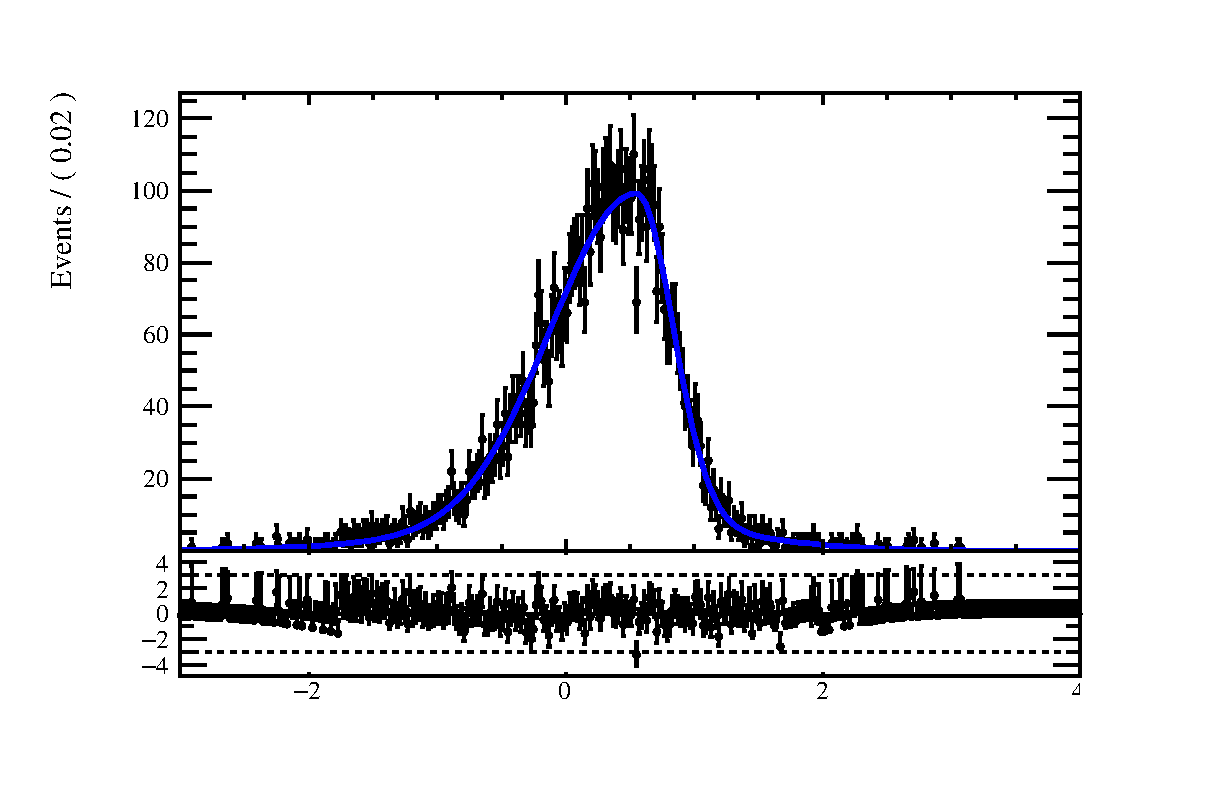
\includegraphics[width=0.75\textwidth]{LbToD0p/fits/MC_D0p_SIG/logIP_RS/fit_DBfG}
	\caption{Fit to the \logIP distribution of the signal simulation. As parametrisation a double Bifurcated Gaussian has been chosen.}
    \label{fig:fit_logIP_signal}
\end{figure}
In order to estimate the quality of the fit, the \textsc{pull} distribution is also shown in Figure \ref{fig:fit_logIP_signal} below the \logIP distribution.
The pull of a variable $x$ is defined as
\begin{align}
    \text{pull}(x) = \frac{N_\text{meas}(x)-N_\text{fit}(x)}{\sigma_{N_\text{meas}}(x)}.  \label{eq:pull}
\end{align}
Referring to Figure \ref{fig:fit_logIP_signal}, $N_\text{meas}(x)$ denotes the number of entries in the bin with $\logIP = x$, $N_\text{fit}(x)$ the corresponding result of the fit in the respective bin and $\sigma_{N_\text{meas}}(x)$ the error on $N_\text{meas}(x)$.
In other words, the pulls are the residuals of the fit normalised to the uncertainty.
If the fit describes the data well, the pull distribution should peak and fluctuate around zero with mean 1 \cite{Pulls}.
From the pull distribution it can be stated that the chosen fit model describes the data well, especially in the tails.
A little bias might be included if on closer looks at the region of $\logIP \approx 0$.

Concerning the \logIP background shape, only a simulation with very little statistics is available.
To get a better idea of the background \logIP shape and to increase statistics, right sign and wrong sign events of this sample have been added.
In this case wrong sign events refers to events with a \Lc\mup in the final state.
Compared to the signal \logIP shape, both, right sign and wrong sign events, describe combinatorial background.
Thus, it is assumed that their \logIP shapes are similar as Figure \ref{fig:plot_logIP_MC_BKG} confirms. 
According to this, the addition of right sign and wrong sign is appropriate to increase statistics in this case.

The \logIP distribution of the background simulation looks lika a Gaussian around the maximum, but has a long tail to lower \logIP values.
That is why a single CrystalBall function is chosen as fit function for the \logIP background shape. 
This function was first used by the CrystalBall collaboration to account for radiative losses in \jpsi or \psitwos decays \cite{CrystalBall}. 
It is defined as 
\begin{align}
    &\CB(x|x_0, \sigma, \alpha, n) \propto
    \begin{cases}
        \exp \left(-\frac{(x-x_0)^2}{2\sigma^2}\right)     & \text{for } \frac{x-x_0}{\sigma} > -\alpha \\
        A \cdot \left(B - \frac{x-x_0}{\sigma}\right)^{-n} & \text{for } \frac{x-x_0}{\sigma} \leq -\alpha
    \end{cases}, \\
    &\text{where} \nonumber\\
    &A = \left(\frac{n}{|\alpha|}\right)^n \exp\left(-\frac{|\alpha|^2}{2}\right), \\
    &B = \frac{n}{|\alpha|} - |\alpha|.
\end{align}
Hence, the CrystalBall function is a Gaussian with an enhanced tail at one side of the maximum, due to the power law for $\frac{x-x_0}{\sigma} \leq -\alpha$.
So $\alpha$ denotes the transition between the Gaussian and the power law tail and $n$ the latter's exponent.

The result of the fit to the background simulation can be seen in Figure \ref{fig:fit_logIP_MC_BKG}.
According to the pull distribution the fit nicely describes the data points.
Nonetheless one has to note that statistics here are very little.
\begin{figure}[tb]
    \centering
	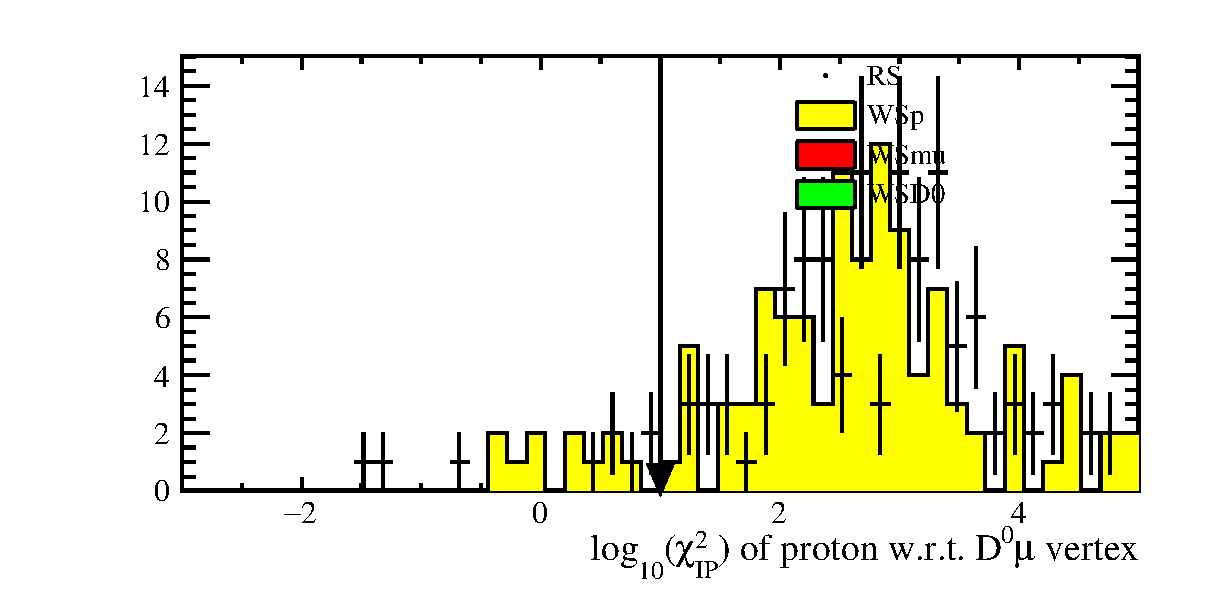
\includegraphics[width=0.75\textwidth]{LbToD0p/plots/MC_B2D0munu_BKG/logIP}
	\caption{Comparison of the \logIP distribution for right sign and wrong sign events in the background simulation. Both, the shapes for right sign and wrong sign are very similar and thus can be added to increase statistics.}
    \label{fig:plot_logIP_MC_BKG}
\end{figure}
\begin{figure}[tb]
    \centering
	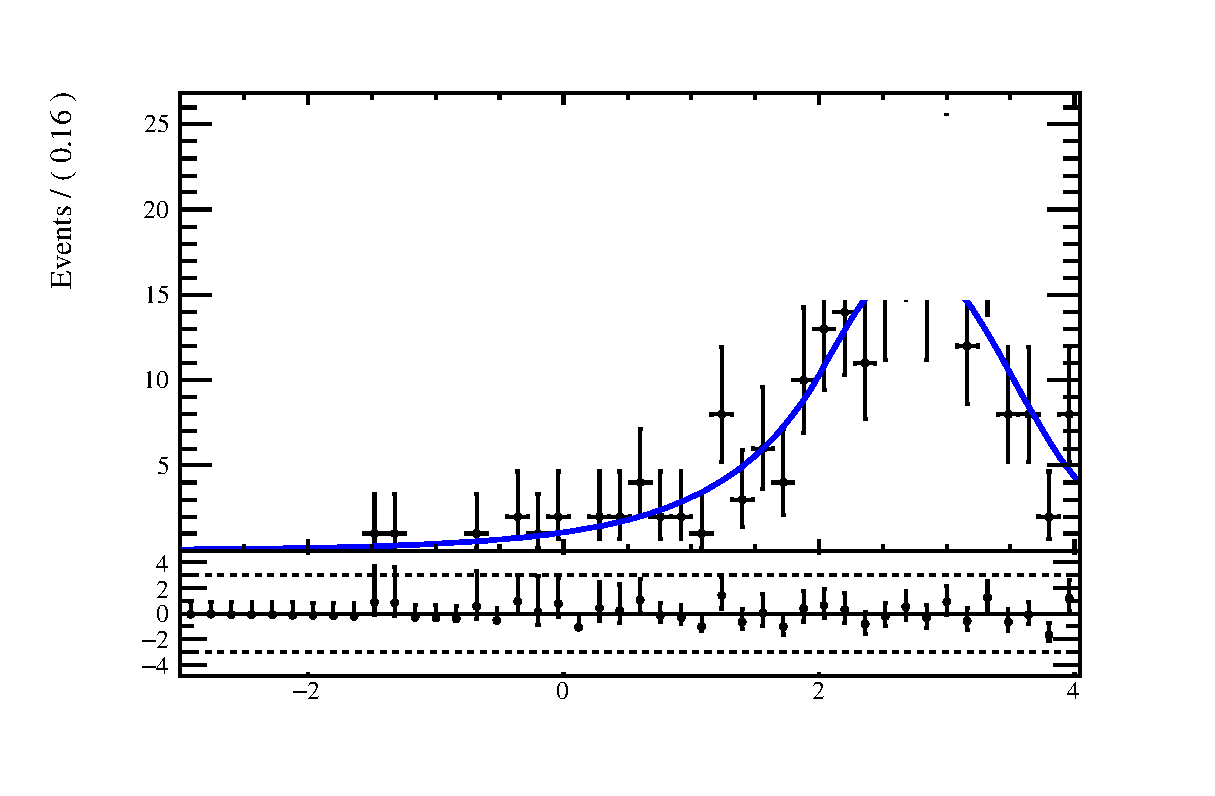
\includegraphics[width=0.75\textwidth]{LbToD0p/fits/MC_B2D0munu_BKG/logIP_RS/fit_CB}
	\caption{Fit to the (RS and WS added) \logIP shape of the background simulation.
             The distribution is modeled with a CrystalBall function.}
    \label{fig:fit_logIP_MC_BKG}
\end{figure}

\subsection{One-dimensional fit to the \logIP distribution in data}
\label{sec:ControlLogIP}
To control if the chosen parametrization of the \logIP distribution gained from simulation describes data, a one-dimensional \logIP-fit on data is performed.
For that purpose, the double bifurcated Gaussian as signal component and the CrystalBall as background component are added, i.e. the total probabiltiy density function $\mathcal{P}$ for that fit is:
\begin{align}
    &\mathcal{P}(x|N_\text{sig}, N_\text{bkg}, x_{0, \text{sig}}, x_{0, \text{bkg}} \vec{\sigmaL{}}_{,\text{sig}}, \vec{\sigmaR{}}_{,\text{sig}}, f_{\BfG_1}, \sigma_\text{bkg}, \alpha, n) \propto \nonumber\\
    &N_\text{sig} \DBfG(x|x_{0, \text{sig}}, \vec{\sigmaL{}}_{,\text{sig}}, \vec{\sigmaR{}}_{,\text{sig}}, f_{\BfG_1}) + N_\text{bkg} \CB(x| x_{0, \text{bkg}}, \sigma_\text{bkg}, \alpha, n)
\end{align},
where $N_\text{sig}$ denotes the signal yield and $N_\text{bkg}$ the background yield respectively.
The fitresult can be seen in Figure \ref{fig:fit_logIP_RS} and the corresponding yields and parameter values are listed in Table \ref{tab:logIP_RS}.
\begin{figure}[tb]
    \centering
	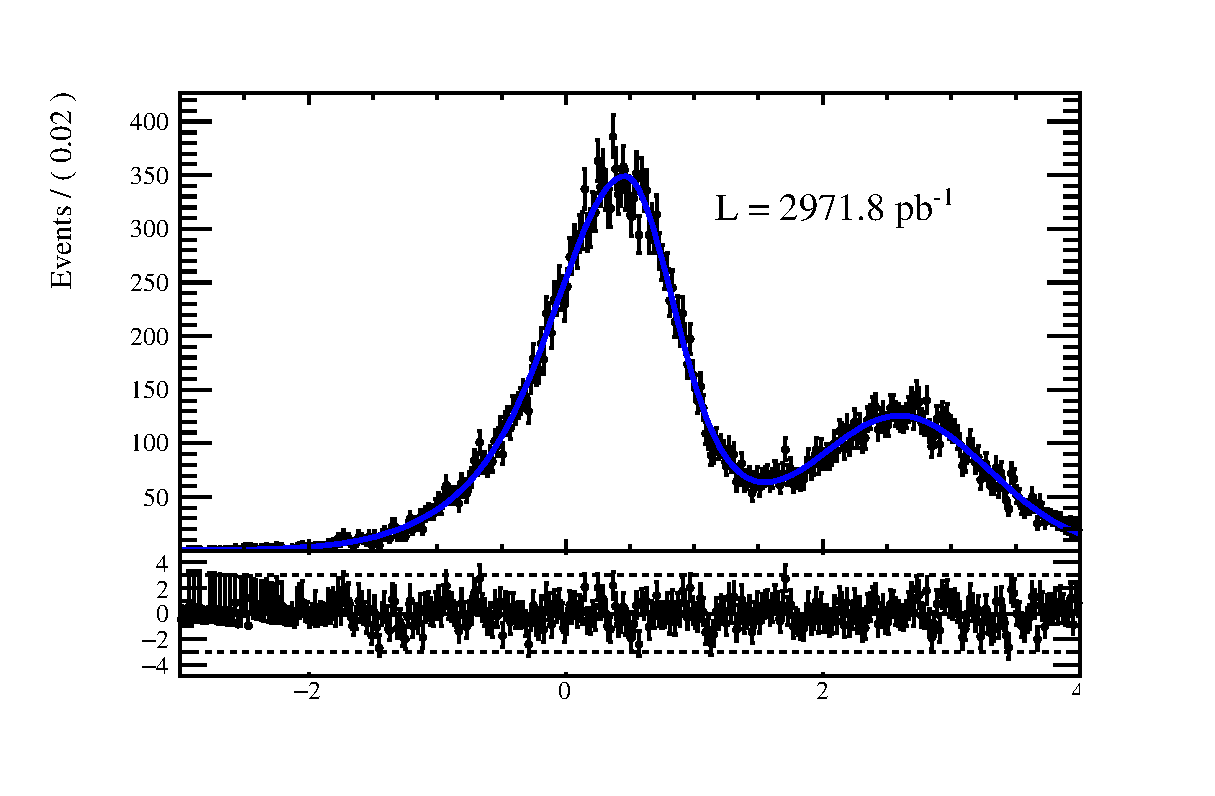
\includegraphics[width=\textwidth]{LbToD0p/fits/data/logIP_RS/fit_DBfG_CB}
	\caption{\logIP distribution of the data sample.
             A binned likelihood fit is performed on it with the sum of a double bifurcated Gaussian for the signal (blue, dashed line) and a CrystalBall function for the background component (yellow shaded). }
    \label{fig:fit_logIP_RS}
\end{figure}
 
\begin{table}[h]
    \centering
    \caption{Results of the onedimensional \logIP fit on data.}
    \label{tab:logIP_RS}
    $\begin{array}{lr@{\pm}l}
    \hline
    \text{Variable} & \multicolumn{2}{c}{\text{Value}} \\
    \hline
        \multicolumn{3}{l}{\text{\textbf{Yields}}} \\
\text{signal yield}&(2.325 & 0.028) \cdot 10^{4}\\
\text{background yield}&(1.086 & 0.026) \cdot 10^{4}\\
\multicolumn{3}{l}{\text{\textbf{Signal (\DBfG)}}} \\
\text{mean}&(4.59 & 0.26) \cdot 10^{-1}\\
\text{left width 1}&(8.72 & 0.56) \cdot 10^{-1}\\
\text{right width 1}&(5.74 & 0.44) \cdot 10^{-1}\\
\text{left width 2}&(4.72 & 0.55) \cdot 10^{-1}\\
\text{right width 2}&(3.37 & 0.23) \cdot 10^{-1}\\
\text{fraction BfG 1}&(5.61 & 0.89) \cdot 10^{-1}\\
\multicolumn{3}{l}{\text{\textbf{Background (\CB)}}} \\
\text{CB mean}&(2.6 & 0.017) \cdot 10^{0}\\
\text{CB $\sigma$}&(6.85 & 0.14) \cdot 10^{-1}\\
\text{CB $\alpha$}&(2.035 & 0.099) \cdot 10^{0}\\
\text{CB $n$}&(1.62 & 0.45) \cdot 10^{0}\\

\hline
\end{array}$
\end{table}
    

The chosen model very nicely describes the data as can be seen in the pull distribution.
Thus the chosen parametrisation for the \logIP shape is reasonable.
This fit is later also used for systematic studies, since it is already able to distinguish between signal and background yields, see Chapter \ref{sec:Selection} for further discussions.

\subsection{\Dz\proton mass shape}
\label{sec:Shape_mD0p}
To get an idea of the (combinatorial) background shape in the \Dz\proton mass distribution, events with a wrong sign proton, i.e. events with \Dz\antiproton\mun in the final state are used since the transition from \Lb to a \Dz\antiproton\mun final state is physically forbidden by charge
conservation and should thus give a good proxy for randomly combined \LbToDpmunu candidates. 
The \MDp distribution of these wrong sign events is shown in Figure \ref{fig:fit_mD0p_WS} and modeled with an empirical background function \cite{EBG}
\begin{align}
    \text{EBG}(m|m_0, m_1, m_2, p,c_1) = \text{PS}(m|m_1,m_2) \cdot (m - m_0)^p \cdot \exp\left[ c_1 \left(1-\frac{m_0}{m}\right)\right], \label{eq:EBG}
\end{align}
where $m_0 := m_1 + m_2$ denotes the kinematic \Dz\proton mass threshold and PS the phase space function
\begin{align}
    \text{PS}(m|m_1,m_2) = \frac{1}{2m} \sqrt{\left[m^2 - (m_1 + m_2)^2\right] \left[m^2 - (m_1 - m_2)^2\right]}. \label{eq:PS}
\end{align}
The term with the power $p$ is included as correction, in case the phase-space function does not satisfactorily describe the threshold shape.
Here and in the following fits, $m_1$ and $m_2$ are fixed to the \Dz respectively proton PDG mass values.
Figure \ref{fig:fit_mD0p_WS} shows the result of the fit.
Again, the model nicely describes the distribution.
It should be noted here, that there is no structure observed in this wrong sign mass spectrum.
This is a good confirmation, that the identification of the two peaks in the \Dz\proton mass for right sign events as \LcResI and \LcResII is appropiate.
\begin{figure}[tb]
    \centering
	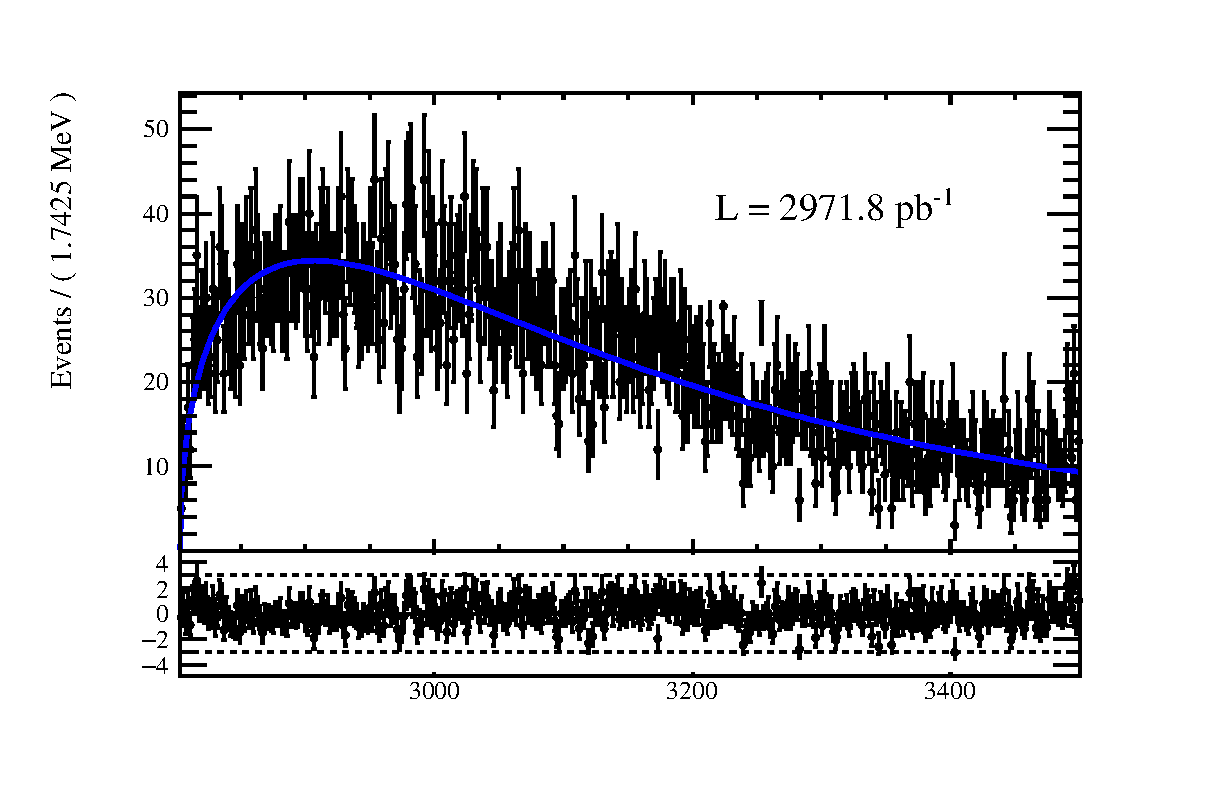
\includegraphics[width=0.75\textwidth]{LbToD0p/fits/data/mD0p_WSp/fit_EmpiricBG}
	\caption{Fit to \Dz\proton mass of wrong sign proton events.
             As model an empiric background function has been chosen, see equation (\ref{eq:EBG})}
    \label{fig:fit_mD0p_WS}
\end{figure}

Unfortunately, there is no reliable simulation predicting the mass shape for the \Dz\proton invariant mass. 
A shape for the signal therefore has to be determined empirically on data. 
A fit to the \Dz\proton mass distribution is applied with the requirement that the \Dz\proton\muon system makes a good vertex, i.e. $\logIP < 1$.
It is shown in Figure \ref{fig:fit_mD0p_RS} top.
This hard requirement strongly suppresses combinatorial background and allows to determine the signal distribution.
As already stated before, the main part of the signal will be nonresonant.
Besides that it is expected to see the two \LcResI and \LcResII resonances.
They are parametrised by a relativistic Breit-Wigner distribution convoluted with a double Gaussian to account for the detector's mass resolution.
The relativistic Breit-Wigner distribution is defined as follows:
\begin{align}
    \text{RelBW}(m|m_R, m_1, m_2, \Gamma_0) \propto 
    \frac{m \Gamma(m|m_R, m_1, m_2, \Gamma_0)}{(m^2-m_R^2)^2 + (m_R \Gamma(m|m_R, m_1, m_2, \Gamma_0))^2}, \label{eq:RelBW}
\end{align}
with 
\begin{align}
    \Gamma(m|m_R, m_1, m_2, \Gamma_0) = \Gamma_0 \frac{m_R}{m} \frac{\PS(m| m_1, m_2)}{\PS(m_R| m_1, m_2)}, 
\end{align}
where PS denotes the phase space function of equation (\ref{eq:PS}), $m_R$ the resonance's mass and $\Gamma_0$ its width \cite{Lb_FF}.
Thus, each resonance is modeled with
\begin{align}
    &\text{RES}(m| m_R, m_1, m_2, \Gamma_0, \sigma_1, \sigma_2, f_1) \propto \nonumber \\
    &\text{RelBW}(m| m_R, m_1, m_2, \Gamma_0) \otimes \left[f_1 \mathcal{G}(m|0,\sigma_1) + (1-f_1) \mathcal{G}(m|0,\sigma_2) \right] \label{eq:RES}
\end{align}
The determination of the mass resolution is thoroughly described in section \ref{sec:Massresolution}. 
The obtained resolution will be fixed in all fits later.

The non-resonant signal part is modeled with the sum of two exponential functions multiplied by a turn-on function.
\begin{align}
    \text{TDExp}(m|m_0, c_0, c_1, c_2, f_{c_1}) \propto \left( 1 - \mathrm{e}^{c_0(m-m_0)} \right) \cdot \left[ f_{c_1} \mathrm{e}^{c_1m} + (1-f_{c_1}) \mathrm{e}^{c_2m} \right]. \label{eq:TDExp}
\end{align}
The turn-on factor is needed to model the steep rise at the \Dz\proton mass threshold.

The fit to the invariant \Dz\proton mass distribution that is shown on the upper side of Figure \ref{fig:fit_mD0p_RS} does not describe the data at low \Dz\proton mass.
Different models for the non-resonant component have been tried to describe this steep curvature without success.
However, when adding another resonant component, the fit converges and describes the data well as can be seen on the lower side of Figure \ref{fig:fit_mD0p_RS}.
This additional component will be labeled ``low mass enhancement" throughout the analysis.
Thus, the total fit function consists of four parts: 
The non-resonant part modeled with the ``turn-on double exponential" function TDExp of eq. (\ref{eq:TDExp}) and relativistic Breit-Wigner functions according eq. (\ref{eq:RES}) for the \LcResI, \LcResII and the low mass enhancement. 
The fit results can be seen in Figure \ref{fig:fit_mD0p_RS} (right) and Table \ref{tab:fit_mD0p_RS}.

Note that at this point, the additional resonant component, the low mass enhancement, is merely introduced to enable the fit to converge and match the data.
There are several possible reasons for such an enhancement.
Nonetheless there is some motivation to choose a resonant model as additional component:
On the one hand the peak looks similar to the other resonances.
On the other hand, there is a similar peak seen in other analyses e.g. \babar is discussing a (much less pronounced) peak at an invariant \Dz\proton mass of about 2840\mev in its study on the \Dz\proton final state in \cite{BaBar_D0p}.
The reason for this peak is not understood so far and is currently studied in different ongoing \lhcb analyses.
Besides some detector effects, backgrounds or kinematical reflections it is not excluded that a new particle is seen here.
A thorough discussion, if this additional component is actually needed and what might cause this peak follows in section \ref{sec:Structure}.
In the following this component is treated as signal since it appears very clear when requiring $\logIP < 1$, i.e. in the background suppressed region making a good decay vertex.
\begin{figure}[tb]
    \centering
	\includegraphics[width=\textwidth]{LbToD0p/fits/data/mD0p_RS/fit_TurnOnDExp_2RelBWPSRes} \\
	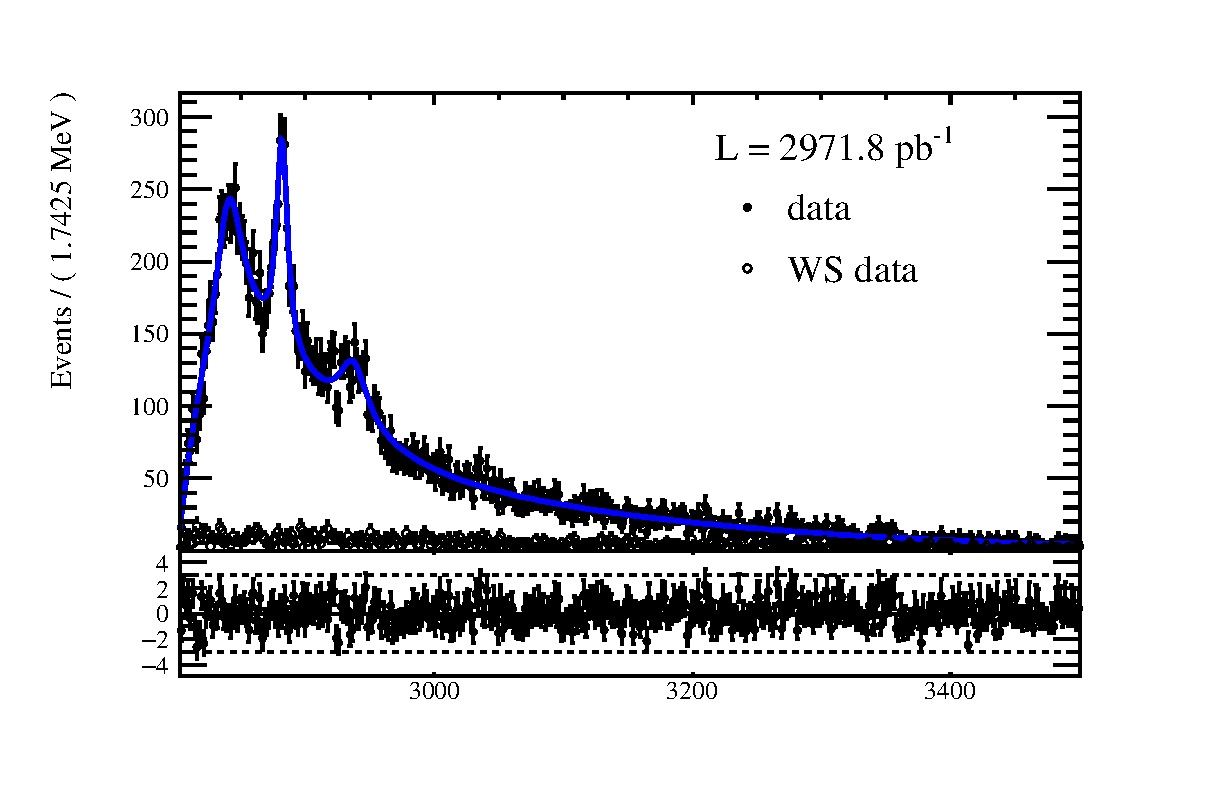
\includegraphics[width=\textwidth]{LbToD0p/fits/data/mD0p_RS/fit_TurnOnDExp_3RelBWPSRes}
	\caption{Invariant \Dz\proton mass distribution when requiring $\logIP < 1$. 
             The upper figure shows a fit with two resonances (red lines) for the \LcResI and \LcResII and a nonresonant part (blue dashed line). 
             Different attempts have been made to get a proper and converging fit, matching the data at low \Dz\proton mass, without success. 
             This issue can be solved by adding an additional resonant component (lower figure, green line), obeying the same fit model like the two resonances.}
    \label{fig:fit_mD0p_RS}
\end{figure}
 
\begin{table}[h]
    \centering
    \caption{Results of the \Dz\proton mass fit.}
    \label{tab:fit_mD0p_RS}
    $\begin{array}{lr@{\pm}l}
    \hline
    \text{Variable} & \multicolumn{2}{c}{\text{Value}} \\
    \hline
        \multicolumn{3}{l}{\text{\textbf{Yields}}} \\
\text{\LcResI signal yield}&(1.35 & 0.16) \cdot 10^{3}\\
\text{\LcResII signal yield}&(1.05 & 0.28) \cdot 10^{3}\\
\text{mass enhancement yield}&(2.24 & 0.36) \cdot 10^{3}\\
\text{nonresonant yield}&(1.681 & 0.063) \cdot 10^{4}\\
\multicolumn{3}{l}{\text{\textbf{\LcResI resonance}}} \\
\text{mean}&(2.88195 & 0.00038) \cdot 10^{3}\\
\text{width}&(10.0 & 6.7) \cdot 10^{0}\\
\multicolumn{3}{l}{\text{\textbf{\LcResII resonance}}} \\
\text{mean}&(2.9364 & 0.0018) \cdot 10^{3}\\
\text{width}&(2.59 & 0.64) \cdot 10^{1}\\
\multicolumn{3}{l}{\text{\textbf{Low mass enhancement}}} \\
\text{mean}&(2.84005 & 0.00086) \cdot 10^{3}\\
\text{width}&(2.41 & 0.32) \cdot 10^{1}\\
\multicolumn{3}{l}{\text{\textbf{nonresonant part}}} \\
\text{turn on mass threshold}&(2.801 & 0.00052) \cdot 10^{3}\\
\text{turn on slope}&(-3.9 & 2.4) \cdot 10^{-3}\\
\text{exponential 1 slope}&(-2.16 & 0.11) \cdot 10^{-2}\\
\text{exponential 2 slope}&(-5.54 & 0.47) \cdot 10^{-3}\\
\text{fraction exponential 1}&(6.84 & 0.55) \cdot 10^{-1}\\

\hline
\end{array}$
\end{table}
    

\section{Determination of the mass resolution}
\label{sec:Massresolution}
Due to resolution effects, the width of a resonance in a mass spectrum can appear wider than its natural width.
In this analysis the effect is accounted for by convoluting the Breit-Wigner, which is assumed to be the natural shape of the resonance, with a double Gaussian, describing the smearing of the resonance due to finite mass resolution, see equation (\ref{eq:RES}).

The determination of the mass resolution is performed in a simulation by comparing the generated (also called ``true") mass with the reconstructed mass.
The mean of the mass difference distribution is expected to be zero and the width refers to the mass resolution.
The distribution is described by a double Gaussian function $f_1 \mathcal{G}(m|m_0,\sigma_1) + (1-f_1) \mathcal{G}(m|m_0,\sigma_2)$ to properly describe the broadening of the mass difference distribution in the tails.
To account for a potential mass dependence, this fit is performed in several bins of the true invariant \Dz\proton mass.
The left-hand side of Figure \ref{fig:massresolution} exemplarily shows the mass difference between reconstructed and generated mass together with the fit of a double Gaussian in the bin $2910 < M(\Dz\proton) < 2980 \mev$.
This bin corresponds to the \LcResII resonance.
The fits of all bins can be seen in Appendix \ref{app:Massresolution}, Figure \ref{fig:massresolution_all}.
The widths $\sigma_1$ and $\sigma_2$ and the fraction of the first Gaussian $f_1$ obtained by these fits in the respective bins are used for the parametrisation of the resonances in the nominal \Dz\proton mass fit as described by equation (\ref{eq:RES}).
Table \ref{tab:Massresolution} summarises the obtained values which are used for the further analysis.
Though there is a mass dependence of the resolution over the whole \Dz\proton mass spectrum it is assumed, that the mass resolution can be considered as constant over the natural width of the resonances.
\begin{table}[tb]
    \centering
    \caption{Results of the fits to the mass difference distributions for the determination of the mass resolution. Only the values, which are required for the further analysis are quoted here.}
    \label{tab:Massresolution}
    $\begin{array}{lr@{\pm}lr@{\pm}lr@{\pm}l}
    \hline
    \text{Resonant component} & \multicolumn{2}{c}{\sigma_1 [\mev]} & \multicolumn{2}{c}{\sigma_2 [\mev]} & \multicolumn{2}{c}{f_1 [\mev]} \\
    \hline
    \LcResI   & \MassresResIwIval & \MassresResIwIerr & \MassresResIwIIval & \MassresResIwIIerr & \MassresResIfIval & \MassresResIfIerr \\
    \LcResII   & \MassresResIIwIval & \MassresResIIwIerr & \MassresResIIwIIval & \MassresResIIwIIerr & \MassresResIIfIval & \MassresResIIfIerr \\
    \text{enhancement} & \MassresStructurewIval & \MassresStructurewIerr & \MassresStructurewIIval & \MassresStructurewIIerr & \MassresStructurefIval & \MassresStructurefIerr \\
    \hline
    \end{array}$
\end{table}
The right-hand side of Figure \ref{fig:massresolution} shows the root-mean-square of the mass difference distributions in the different bins.
This serves as a measure for the mass resolution and how it evolves since it is hard to assign a single value for the mass resolution due to the fit of a double Gaussian.
At \Dz\proton mass threshold, the \Dz and the proton are at rest.
Thus, the measured \Dz\proton mass is just the sum of the PDG masses of the \Dz and the proton.
Hence, there is no sensitivity to a mass resolution at threshold.
If the measured \Dz\proton mass is above the threshold, there are contributions from the momenta of the \Dz and the proton to the measured \Dz\proton mass, too, influencing the mass resolution.
As the uncertainties of the momenta gets larger for increasing momenta, the mass resolution increases as well.
\begin{figure}[tb]
    \centering
	\includegraphics[width=0.49\textwidth]{LbToD0p/massresolution/massresolution_03}
	\includegraphics[width=0.49\textwidth]{LbToD0p/massresolution/massresolution_widths}
	\caption{Left: Fit of a Gaussian to the difference between generated and reconstructed \Dz\proton mass of the simulation sample in the range $2910 < M(\Dz\proton) < 2980 \mev$, corresponding to the bin of the \LcResII resonance. Right: root-mean-square (RMS) of the mass difference distributions for each bin.
    The RMS serves as a measure for the mass resolution since it is not easy to assign a single value for the mass resolution, since the distribution is modeled with a double Gaussian.}
    \label{fig:massresolution}
\end{figure}


\section{Nominal fit in two dimensions}
\label{sec:Fit_2D}
With a two-dimensional fit to the \Dz\proton mass and the \logIP distribution it is possible to distinguish between nonresonant signal and background in the \Dz\proton mass spectrum as already explained.
Thus, the different pieces of the previous sections are put together for a fit of both distributions.

It is assumed that the \logIP distribution is the same for all 4 different signal components (non-resonant signal, \LcResI, \LcResII, enhancement), since their decay topologies are the same\footnote{Presumed, that the enhancement indeed emerges to be a resonance or another signal component.}.
Hence, their \logIP distributions share all parameters. 
For the \logIP signal part a double Bifurcated Gaussian \DBfG is chosen, whereas the background is modeled by a CrystalBall function \CB.
The \Dz\proton mass' signal components are modeled with the same parametrisation as described in section \ref{sec:Shape_mD0p}. 
The empiric background function EBG is used to describe the background.
Thus, the total parametrisation $\mathcal{P}_\text{2D}$ of the two-dimensional \logIP/\MDp distribution is
\begin{align}
    & \mathcal{P}_\text{2D}(x, m | \vec{\lambda}) \propto \nonumber \\
    & \DBfG(x|x_{0, \text{sig}}, \vec{\sigma}_{\text{L,sig}}, \vec{\sigma}_{\text{R,sig}}, f_{\BfG_1}) \nonumber \\
    & \quad \cdot \left[\phantom{+} N_\text{nonres} \cdot \text{TDExp}(m|m_0, c_0, c_1, c_2, f_{c_1}) \right. \nonumber \\
    & \quad \phantom{\cdot [} + N_{\LcResI} \cdot \RES(m| m_{\LcResI}, m_1, m_2, \Gamma_{0, \LcResI}, \vec{\sigma}_{\LcResI}, f_{1, \LcResI}) \nonumber \\
    & \quad \phantom{\cdot [} + N_{\LcResII} \cdot \RES(m| m_{\LcResII}, m_1, m_2, \Gamma_{0, \LcResII}, \vec{\sigma}_{\LcResII}, f_{1, \LcResII}) \nonumber \\
    & \quad \phantom{\cdot [} + N_\text{enh} \cdot \RES(m| m_\text{enh}, m_1, m_2, \Gamma_{0, \text{enh}}, \vec{\sigma}_{\text{enh}}, f_{1, \text{enh}})\left.\right] \nonumber \\
    & + \CB(x| x_{0, \text{bkg}}, \sigma_\text{bkg}, \alpha, n) \cdot N_\text{bkg} \cdot \text{EBG}(m|m_0, m_1, m_2, p,c_{1, \text{bkg}}),
\end{align}
where $x$ denotes \logIP, $m$ the invariant \Dz\proton mass, $\vec{\lambda}$ the set of all fit parameters and $N_i$ the yields of the respective components.
All other parameters are explained in the sections before, where the different functions have been introduced.
All parameters are floating except for the mass resolution parameters of the resonant components in \RES(...) and the \Dz and proton mass ($m_1$ respectively $m_2$), that are required in the phase space function PS, which again is part of the relativistic Breit-Wigner and the empiric background function. 
The results of the fit are shown in Table \ref{tab:2Dfit} and the projections can be seen in Figure \ref{fig:fit2D}.
The model very nicely describes the data.
The pull distributions do not show any abnormalities.
A discussion of the result follows in section \ref{sec:Signalyield_D0p}.
\begin{figure}[tb]
	\centering
	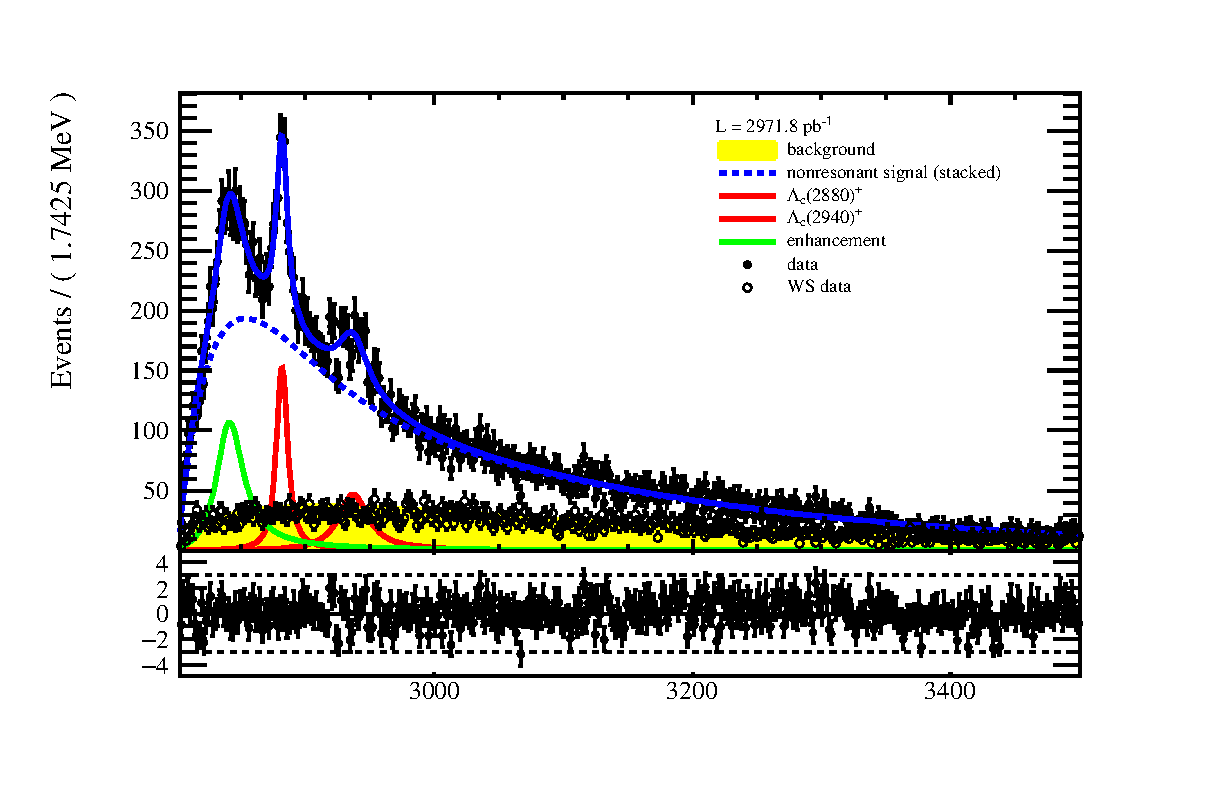
\includegraphics[width=\textwidth]{LbToD0p/fits/data/2Dfit/fit_DBfG_CB_vs_TurnOnDExp_3RelBWPSRes_EmpiricBG_mD0pProj} \\
	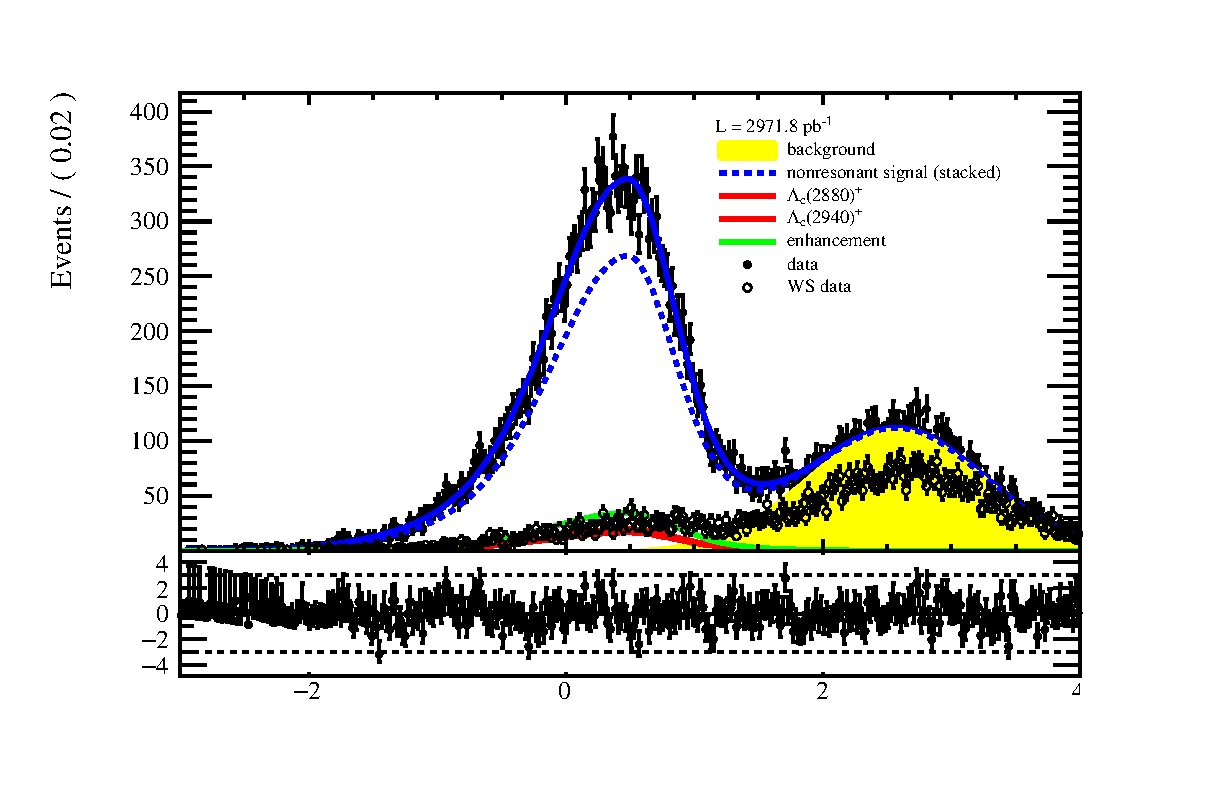
\includegraphics[width=\textwidth]{LbToD0p/fits/data/2Dfit/fit_DBfG_CB_vs_TurnOnDExp_3RelBWPSRes_EmpiricBG_logIPProj}
	\caption{Two-dimensional fit to the \LbToDpmunuX candidates. Top: projection of invariant \Dz\proton mass. Bottom: projection of \logIP distribution projection.
             The fit model is described in the text.
             The yellow shaded area shows the background component, stacked on top the non-resonant signal component marked as blue, dashed line.
             The two identified \LcResI and \LcResII resonances are drawn with a red solid line, the additional enhancement in green.
             For comparison the open circles show the wrong sign events.}
	\label{fig:fit2D}
\end{figure}
 
\begin{table}[h]
    \centering
    \caption{Results of the twodimensional M(\Dz\proton) and \logIP fit.}
    \label{tab:2Dfit}
    $\begin{array}{lr@{\pm}l}
    \hline
    \text{Variable} & \multicolumn{2}{c}{\text{Value}} \\
    \hline
        \multicolumn{3}{l}{\text{\textbf{Yields}}} \\
\text{\LcResI signal yield}&(1.34 & 0.15) \cdot 10^{3}\\
\text{\LcResII signal yield}&(1.13 & 0.23) \cdot 10^{3}\\
\text{mass enhancement yield}&(2.39 & 0.44) \cdot 10^{3}\\
\text{nonresonant signal yield}&(1.807 & 0.067) \cdot 10^{4}\\
\text{background yield}&(9.42 & 0.14) \cdot 10^{3}\\
\multicolumn{3}{l}{\text{\textbf{\LcResI resonance}}} \\
\text{mean [\mev]}&(2.88185 & 0.00034) \cdot 10^{3}\\
\text{width [\mev]}&(8.8 & 1.3) \cdot 10^{0}\\
\multicolumn{3}{l}{\text{\textbf{\LcResII resonance}}} \\
\text{mean [\mev]}&(2.9367 & 0.0017) \cdot 10^{3}\\
\text{width [\mev]}&(2.7 & 0.5) \cdot 10^{1}\\
\multicolumn{3}{l}{\text{\textbf{Low mass enhancement}}} \\
\text{mean [\mev]}&(2.84016 & 0.00087) \cdot 10^{3}\\
\text{width [\mev]}&(2.53 & 0.34) \cdot 10^{1}\\
\multicolumn{3}{l}{\text{\textbf{Nonresonant signal}}} \\
\text{turn on mass threshold [\mev]}&(2.80123 & 0.0006) \cdot 10^{3}\\
\text{turn on slope [\mev$^{-1}$]}&(-1.3 & 4.0) \cdot 10^{-4}\\
\text{exponential 1 slope [\mev$^{-1}$]}&(-2.36 & 0.12) \cdot 10^{-2}\\
\text{exponential 2 slope [\mev$^{-1}$]}&(-7.09 & 0.26) \cdot 10^{-3}\\
\text{fraction exponential 1}&(7.32 & 0.21) \cdot 10^{-1}\\
\multicolumn{3}{l}{\text{\textbf{Background (mass)}}} \\
\text{Empiric BG $c_1$ [\mev$^{-1}$]}&(-1.595 & 0.05) \cdot 10^{1}\\
\text{Empiric BG $p_0$}&(5.6 & 3.0) \cdot 10^{-2}\\
\multicolumn{3}{l}{\text{\textbf{Signal (\logIP)}}} \\
\text{mean}&(4.8 & 0.16) \cdot 10^{-1}\\
\text{left width 1}&(9.76 & 0.29) \cdot 10^{-1}\\
\text{right width 1}&(6.23 & 0.33) \cdot 10^{-1}\\
\text{left width 2}&(5.38 & 0.25) \cdot 10^{-1}\\
\text{right width 2}&(3.41 & 0.15) \cdot 10^{-1}\\
\text{fraction BfG 1}&(4.2 & 0.45) \cdot 10^{-1}\\
\multicolumn{3}{l}{\text{\textbf{Background (\logIP)}}} \\
\text{CB mean}&(2.573 & 0.012) \cdot 10^{0}\\
\text{CB $\sigma$}&(6.87 & 0.11) \cdot 10^{-1}\\
\text{CB $\alpha$}&(5.8 & 4.1) \cdot 10^{0}\\
\text{CB $n$}&(1.0 & 1.5) \cdot 10^{0}\\

\hline
\end{array}$
\end{table}
    

% ==================================
% Subsection: Control of the method
% ==================================
\section{Fit to the wrong sign proton data as cross-check}

As a cross-check the two-dimensionsal fit is performed for the wrong sign data with the same parametrisation as for the right sign data in section \ref{sec:Fit_2D}.
However, due to the absence of resonances it is purely described by the nonresonant functions, i.e. the nonresonant signal component and the background component.
The respective plots can be seen in Figure \ref{fig:fit_2D_WS}. 
No structure in the mass distribution is seen, especially the \LcResI and \LcResII resonances vanish in the wrong sign \Dz\proton.
Interesting is to note, that besides the two resonances even the enhancement vanishes.
Thus, it cannot be explained by random combinations of the particles.
Concerning the \logIP distribution, there is nevertheless a ``signal-like" part. 
This is presumably background from \BToDmunuX decays, where the $X$ is of ``wrong charge" and moreover misidentified as (anti)proton.
Since the physics are different for right sign and wrong sign events, the yield obtained in this WS fit cannot easily be subtracted from the nominal fit to account for fake proton backgrounds.
A more thorough study on fake backgrounds will be performed in Chapter \ref{sec:Backgrounds}.
\begin{figure}[tb]
	\centering
	\includegraphics[width=0.49\textwidth]{LbToD0p/fits/data/2DWSfit/fit_DBfG_CB_vs_TurnOnDExp_EmpiricBG_mD0pProj}
	\includegraphics[width=0.49\textwidth]{LbToD0p/fits/data/2DWSfit/fit_DBfG_CB_vs_TurnOnDExp_EmpiricBG_logIPProj}
	\caption{Invariant \Dz\proton mass (left) and \logIP (right) distribution for ``wrong sign" (WS) events.
             The signal-like component (blue, dashed line) of the fit can be assigned to \BToDmunuX decays, where the $X$ is a fake proton of ``wrong" charge.}
	\label{fig:fit_2D_WS}
\end{figure}


% ==================================
% Section: Signal yield and resonances
% ==================================
%\section{Extraction of \LbToDpmunuX signal yield together with \LcResI and \LcResII properties}
\section{Extraction of \LbToDpmunuX signal yield and \LcResI / \LcResII properties}
\label{sec:Signalyield_D0p}
From the previous fits different results can be obtained. 
The most important result is the \LbToDpmunuX signal yield \NDp for the determination of \R.
This result is obtained by the nominal two-dimensional fit.
The obtained yields for the non-resonant component, the \LcResI and the \LcResII as well as the enhancement, which can be found in Table \ref{tab:2Dfit} are summed up.
Thus, the total \LbToDpmunuX signal yield is
\begin{align*}
    \NDp &= N_{\text{nonres}} + N_{\LcResI} + N_{\LcResII} + N_{\text{enh}} \\
         &= (\NDpvalscient \pm \NDperrscient)\cdot 10^{\NDpexpscient}. 
\end{align*}
Remember, that the aim of this thesis is to measure the inclusive branching ratio of \LbToDpmunuX.
That is why all components ending up in a final state containing a \Dz, a proton and a muon are taken summed up for the total signal yield.
Again, it has to be confirmed in chapter \ref{sec:Structure}, that it is appropriate to consider the enhancement as signal.

As a side effect, the properties of the \LcResI and \LcResII resonances are extracted from the fit of the invariant \Dz\proton mass.
In this case it is not needed to distinguish between nonresonant signal and background, since only the peaks are of interest. 
To avoid uncertainties caused by this distinction, the properties of the two resonances are taken from the one-dimensional fit to the invariant \Dz\proton mass (see Table \ref{tab:fit_mD0p_RS}):
\begin{align*}
    \LcResI: \qquad  m_{\LcResI}       &= (\LcResImeanval \pm \LcResImeanerr) \mev, \\
                     \Gamma_{\LcResI}  &= (\LcResIwidthval \pm \LcResIwidtherr) \mev, \\
    \LcResII: \qquad m_{\LcResII}      &= (\LcResIImeanval \pm \LcResIImeanerr) \mev, \\
                     \Gamma_{\LcResII} &= (\LcResIIwidthval \pm \LcResIIwidtherr) \mev.
\end{align*}
The PDG values for the properties of the two resonances are $m_{\LcResI, \text{PDG}} = (2881.53 \pm 0.35)\mev$ and $\Gamma_{\LcResI, \text{PDG}} = (5.8 \pm 1.1)\mev$ for the \LcResI as well as $m_{\LcResII, \text{PDG}} = (2939.3^{+1.4}_{-1.5})\mev$ and $\Gamma_{\LcResII, \text{PDG}} = (17^{+8}_{-6})\mev$ for the \LcResII respectively.
These values are based on a \babar measurement of the \Dz\proton final state and a \belle measurement of \LcResI/\LcResII decays into $\Sigma_\cquark(2455)^{0,++}\pipm$ \cite{Belle_LcRes}.
The obtained results are in good agreement with the current world averages.

Though the reason for the low mass enhancement is not understood so far and it cannot be concluded if a new particle is seen, the obtained mass and width should be quoted here for the sake of completeness:
\begin{align*}
    \text{enhancement}: \qquad  m_{\text{enh}} &= (\Structuremeanval \pm \Structuremeanerr) \mev, \\
                                \Gamma_{\text{enh}}   &= (\Structurewidthval \pm \Structurewidtherr) \mev.
\end{align*}

  \chapter{Normalisation fit}
\label{sec:Normalisationfit}
This chapter describes the measurement of the signal yield \NLc in the normalisation channel \LbToLcmunu (\LcTopKpi). 
The method is different to the one in the signal channel \LbToDpmunuX due to several reasons:
All of the final state particles of the subdecay \LcTopKpi can be reconstructed and the statistics is much higher. 
Going through an intermediate resonance it is possible to see a clear \Lc mass peak as shown in figure \ref{fig:plot_Lc_M}.
In \LbToDpmunuX the major part of the decays was non-resonant.
The small sidebands indicate a small combinatorial background in the subdecay \LcTopKpi.
The background contribution coming from a random combination of a \Lc with a muon can be estimated by investigating the wrong sign final states combinations \Lc\mup.
Since a \Lb can't decay into a \Lc\mup due to charge conservation, this unphysical combination serves a model for randomly combined \Lc\mun.
The second reason why a different method is chosen compared to the \LbToDpmunuX channel is the fact that the \Lb can decay in several excited \Lc states, in the following denoted as \Lcstar for any excited \Lc state.
It has been shown in \ref{SL_Vub} that the \LbToLcmunu data is saturated by the decays \decay{\Lb}{\LcRes{(2595)}\mun\neumb} and \decay{\Lb}{\LcRes{(2625)}\mun\neumb}.
These excited \Lcstar baryons instantly decay for instance in \Lc\pip\pim or \Lc\piz. 
If these pions are not reconstructed, this decay cannot be distinguished from \LbToLcmunu by its topology.
That is why a fit of \logIP does not make any sense here and a different approach for the determination of \NLc has to be chosen.
The solution of the latter problem is to fit the corrected \pKpi\mun, i.e the visible \Lb mass.
It has been stated in chapter \ref{sec:Selection}, that the corrected \pKpi\mun or \Lb mass peak at the nominal \Lb mass, if the missing particle is massless.
Concerning the \decay{\Lb}{\Lcstar\mun\neumb} decays, on misses not only the neutrino, but furthermore massive particles like the pions.
Thus, the corrected \Lb mass is shifted to lower mass, enabling a fit to distinguish between the semileptonic \Lb decay into a \Lc or \Lcstar.
This assumption on the corrected mass is verified in section \ref{sec:FitCorrectedMass}.
\begin{figure}[hptb]
    \centering
	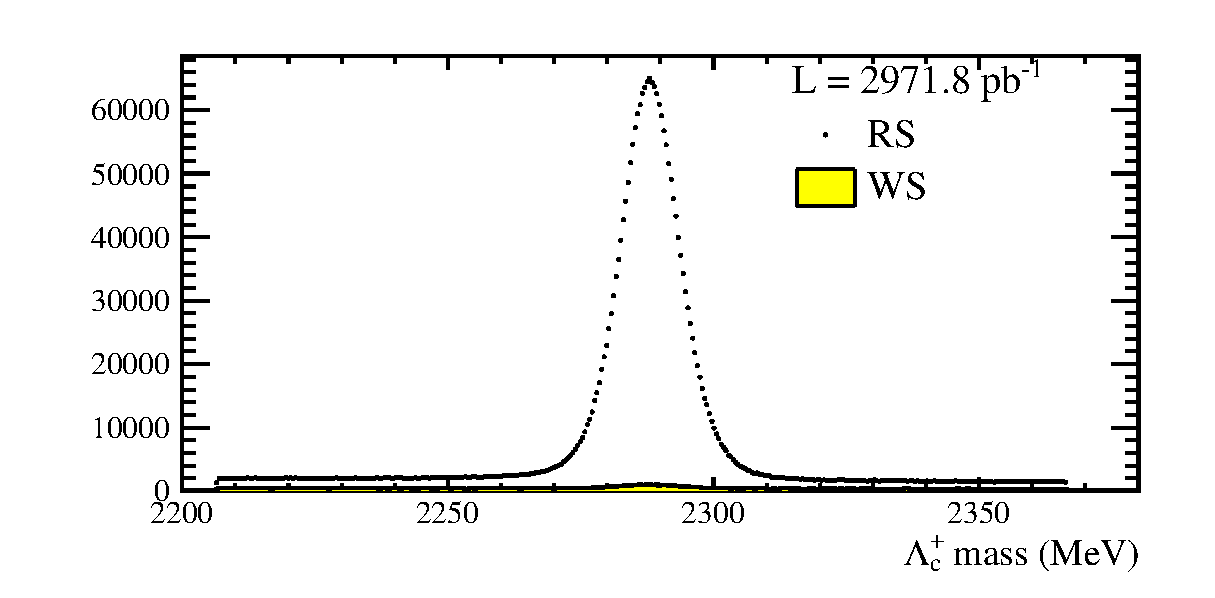
\includegraphics[width=\textwidth]{LbToLc/plots/data/Lc_M}	
	\caption{Plot of the invariant \pKpi mass distribution. A clear mass peak identified as the \Lc can be seen. The yellow shaded area shows events with the WS combination \Lc\mup.}
	\label{fig:plot_Lc_M}
\end{figure}

\section{Reduction and handling of backgrounds}
This section describes the ways how different sources of backgrounds are either handled or reduced.

\subsection{Non \Lc background}
As already mentioned the reconstruction of \pKpi yields a nice mass peak forming the hadronically decaying \Lc, which can be seen in figure \ref{fig:plot_Lc_M}. 
Events outside of this peak can be explained by a random combination of a proton, a kaon and a pion.
Nonetheless there is also a certain amount of this ``combinatorial" background in the peak region.
It is statistically eliminated by a sideband subtraction (see section \ref{sec:Sidebandsubtraction}).
The signal band is chosen to lie in the invariant \pKpi mass range between $\in \left[2260, 2320\right]\mev$.
The background bands are M(\pKpi) $\in \left[2225, 2260\right]\mev$ or M(\pKpi) $\in \left[2320, 2345\right]\mev$.

\subsection{Random combinations of \Lc and \mun}
The next possible source of backgrounds are random combinations of a \Lc baryon and a \mun. 
Due to the missing neutrino \neumb there is no signal mass peak and it is not possible to use a sidebandsubtraction on the invariant \pKpi\mun (\Lc\mun) mass.
Thus, wrong sign events, i.e. ``unphysical" events with a \Lc\mup in the final state as explained above are used to estimate the amount of random \Lc\mun background.
It is assumed that the shape and the number of the wrong sign events are compatible with the shape and number of random \Lc\mun combinations.
Finally, the wrong sign events are subtracted from the ``right sign" events to eliminate this source of backgrounds.

\subsection{Peaking backgrounds}
The third source of backgrounds is peaking background from partially reconstructed decays.
This means that there are physical decays mimicking to be signal since some of the particles are not reconstructed.
In this case the data is saturated by the decays \decay{\Lb}{\LcstarRes{(2595)}\mun\neumb} and \decay{\Lb}{\LcstarRes{(2625)}\mun\neumb} \cite{SL_Vub}.
A \Lcstar subsequently decays into a \Lc and not reconstructed neutral remnant, e.g. \piz, \pip\pim.
Since this decay happens instantaneously it looks the same as \LcTopKpi in the detector.
As already explained, those decays can be distinguished from \LbToLcmunu by their corrected \Lb mass.
Thus, these kind of backgrounds are not subtracted from the data, but rather included as component into the fit to the corrected \Lb mass.

\section{Fit to the corrected \pKpi\mun (\Lb) mass}
\label{sec:FitCorrectedMass}
In this chapter it is verified in simulations, that the corrected \pKpi\mun mass is different for \LbToLcmunu, \decay{\Lb}{\LcstarRes{(2595)}\mun\neumb} and \decay{\Lb}{\LcstarRes{(2625)}\mun\neumb}.
Figure \ref{fig:correctedMass_normalisation} shows the simulated corrected \pKpi\mun mass distributions for the different decays.
\begin{figure}[hptb]
	\centering
	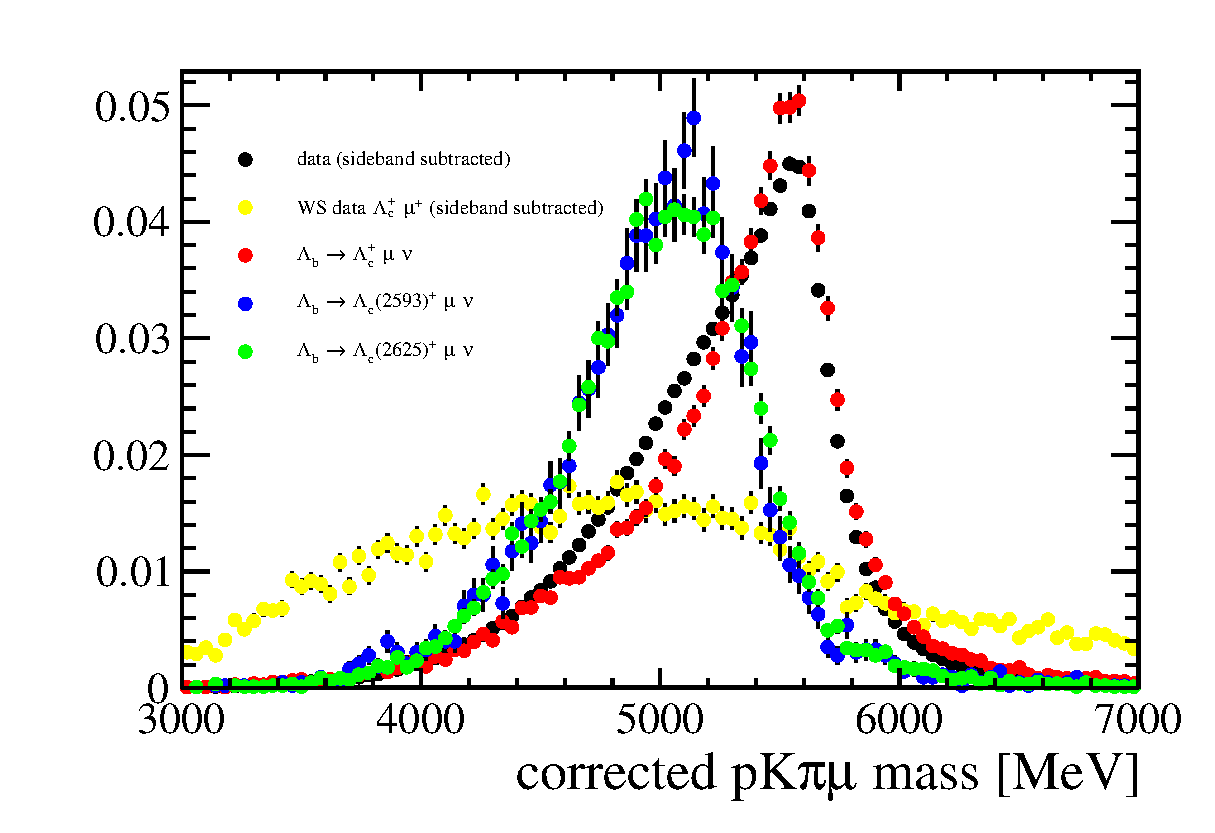
\includegraphics[width=0.75\textwidth]{LbToLc/correctedMass/correctedMass}
	\caption{Comparison of the \pKpi\mun corrected mass for the semileptonic \Lb decays via \Lc, \LcstarRes{(2593)} and \LcstarRes{(2625)} gained from simulation. The black points show the sideband subtracted data distribution. The shape of combinatorial \Lc\mun background (WS events) is shown in yellow.}
	\label{fig:correctedMass_normalisation}
\end{figure}

With the help of Figure \ref{fig:correctedMass_normalisation}, one can draw the following conclusions:
\begin{itemize}
    \item The corrected \pKpi\mun mass indeed looks different for \LbToLcmunu and \decay{\Lb}{\Lcstar\mun\neumb} decays.
          It peaks around the nomimal \Lb mass for \LbToLcmunu whereas it is shifted to lower masses for the decays into the excited \Lcstar states. 
    \item It is not possible to distinguish between the semileptonic \Lb decays into \LcstarRes{(2595)} and \LcstarRes{(2625)} as their shapes are too similar.
\end{itemize}
The latter conclusion is not really a problem since the only result of interest is the \LbToLcmunu signal yield. 
A distinction among the excited states is not needed.
In the fit there will be just one common component for both final states.
Having this in mind, the fit procedure is performed as follows:
\begin{enumerate}
    \item The data is sideband-subtracted in the \pKpi (i.e. \Lc) mass bands.
    \item The corrected \pKpi\mun mass distribution from wrong sing events is subtracted from the respective distribution from the right sign data.
    \item A fit of the \pKpi\mun mass is performed using the Beeston-Barlow method (see sec. \ref{sec:BeestonBarlow}) to account for uncertainties in the corrected mass templates from simulation. The fitted parameters are the \Lc signal yield and one common yield for the two excited \Lcstar channels.
\end{enumerate}
The results can be seen in figure \ref{fig:correctedMass_fit} and table \ref{tab:fit_correctedMass}. 
They are presented in different ways:
The left-hand side shows the fit result with the Beeston-Barlow adjusted templates, i.e. the templates have been modified binwise within their uncertainties to better match the data.
The agreement with the data is remarkable, even on a logarithmic scale, shown in the bottom row of Figure \ref{fig:correctedMass_fit}.
The right-hand side compares data and fitresult with the bare templates.
Slight deviations can be figured out here, above all in the tails with few statistics.
The \LbToLcmunu signal yield \NLc obtained by the fit to the corrected \pKpi\mun mass and required for the determination of \R is:
\begin{align*}
    \NLc = (\NLcvalscient \pm \NLcerrscient)\cdot 10^{\NLcexpscient}
\end{align*}
\begin{figure}[hptb]
	\centering
	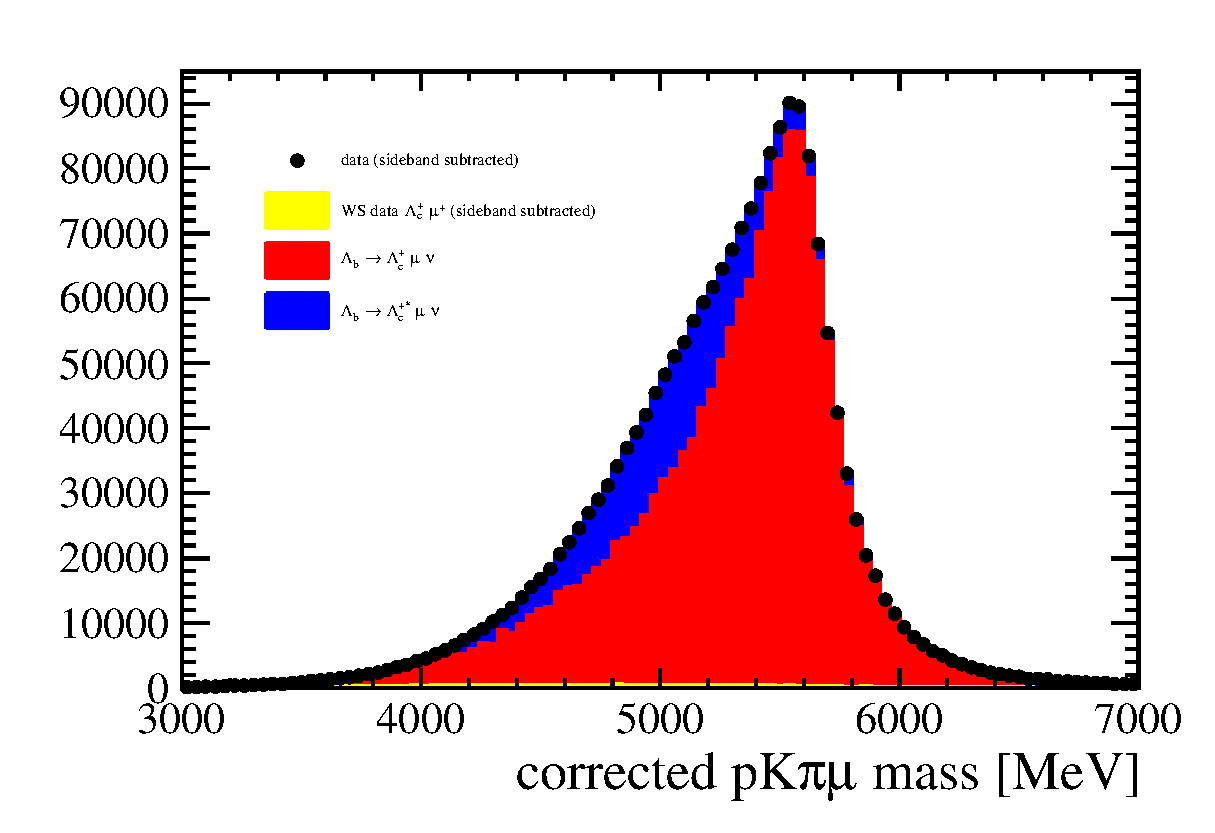
\includegraphics[width=0.49\textwidth]{LbToLc/correctedMass/fit_correctedMass}
	\includegraphics[width=0.49\textwidth]{LbToLc/correctedMass/fit_correctedMass_noBB} \\
	\includegraphics[width=0.49\textwidth]{LbToLc/correctedMass/fit_correctedMass_logscale}
	\includegraphics[width=0.49\textwidth]{LbToLc/correctedMass/fit_correctedMass_noBB_logscale}
	\caption{Fit to the \pKpi\mun corrected mass for the determination of the \LbToLcmunu signal yield. The left plot shows the fit result with the Beeston-Barlow adjusted templates, the right one the bare templates without any modification. The top row shows the result on a linear, the bottom row on logarithmic scale.}
	\label{fig:correctedMass_fit}
\end{figure}
 
\begin{table}[h]
    \centering
    \caption{Results of the \Lc corrected mass fit.}
    \label{tab:fit_correctedMass}
    $\begin{array}{lr@{\pm}l}
    \hline
    \text{Variable} & \multicolumn{2}{c}{\text{Value}} \\
    \hline
        \text{\Lc candidates \NLc}&(1.5837 & 0.0098) \cdot 10^{6}\\
\text{excited \Lcstar candidates}&(3.849 & 0.087) \cdot 10^{5}\\
\text{combinatoric background}&(3.406 & 0.026) \cdot 10^{4}\\

\hline
\end{array}$
\end{table}
    

  \chapter{Efficiencies}
\label{sec:Efficiencies}

The detection and reconstruction of particle decys is not perfect at all, i.e. not all particles and tracks happening in succession of a \proton\proton interaction are detected and recorded.
This discrepancy between the measured signal yields and the actually happened decays is summarized with the term ``efficiencies".
There are several reasons why different kinds of efficiencies occur.
Here are some examples:
\begin{itemize}
    \item Particles are flying out of the detector.
    \item A particle traverses a sensor in the deadtime, i.e. a signal caused by an earlier particle is still processed. 
          In this time, the sensor isn't able to process the second signal.
    \item Applying cuts for the reduction of background prevents signal events to pass these cuts as well
    \item ...
\end{itemize}
It's obvious that this list above is only the tip of the iceberg.
Nonetheless it's crucial to account for these efficiencies if one measures a physical quantity reliant on the number of events.
The way how the efficiencies for the \LbToDpmunuX and \LbToLcmunu enter the measurement of the relative branching ratio \R is shown in equation (\ref{eq:R}).

The determination of the efficiencies requires the use of simulations.
These simulation samples contain informations about all generated events as well as reconstructed events after the simulation of the detector. 
The naive way would be to divide the number of reconstructed MC events after applying all selection cuts and divide this by the number of generated events. 
This efficiency is hereafter called selection efficiency \effSel.
Nonetheless, the generation of the events isn't efficient at all. 
Several requirements are already applied during generation to reduce the computation time of the simulation production.
Above all the simulation of the detector takes a lot of time.
That's why all generated events are required to be in the \lhcb aceptance.
A further acceleration of the production process can be achieved with additional requirements on the final state particles' (transverse) momenta.
Concerning the  \LbToDpmunuX and \LbToLcmunu channel these requirements are different and likewise the efficiencies of the genration process.
Thus, the so called generator level efficiency \effGen also has to determined for both channels. 
The total efficiency used for the calculation of \R is then the product $\effGen \cdot \effSel$.

As life is not that easy the simulations don't perfectly describe the data. 
Above all the \LbToDpmunuX signal simulation doesn't contain a proper physics description and is thus in disagreement with data. 
Unfortunately, no theory prediction of the \LbToDpumnuX channel is available to fix this problem.
The plots in figure \ref{fig:reweighting} show a comparison of data (black points) and the simulation (red lines).
To get a better description of the decay the simulation hence has to be reweighted.
This should lead to a more proper estimate of the efficiency.
Several reweigthing steps are applied and will be described in the following.
\begin{figure}[hptb]
	\centering
	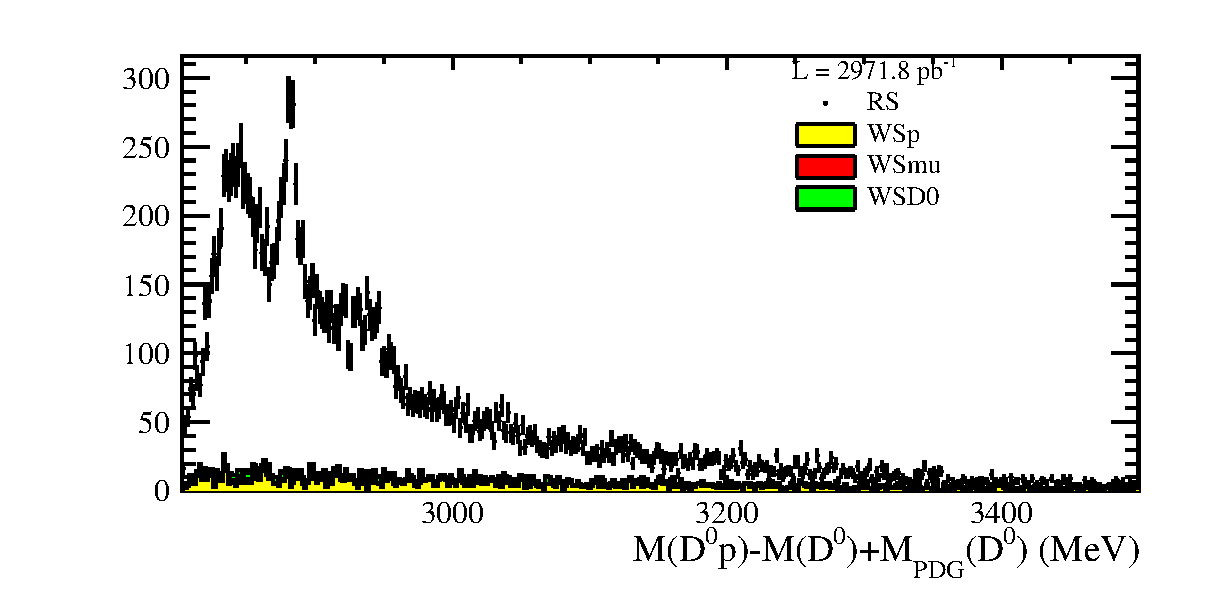
\includegraphics[width=0.49\textwidth]{LbToD0p/comparisons/3D/mD0p_mD0mu_mD0pmu/20Bins/20.0MaxWeight/Bh_DELTA_MASS}
	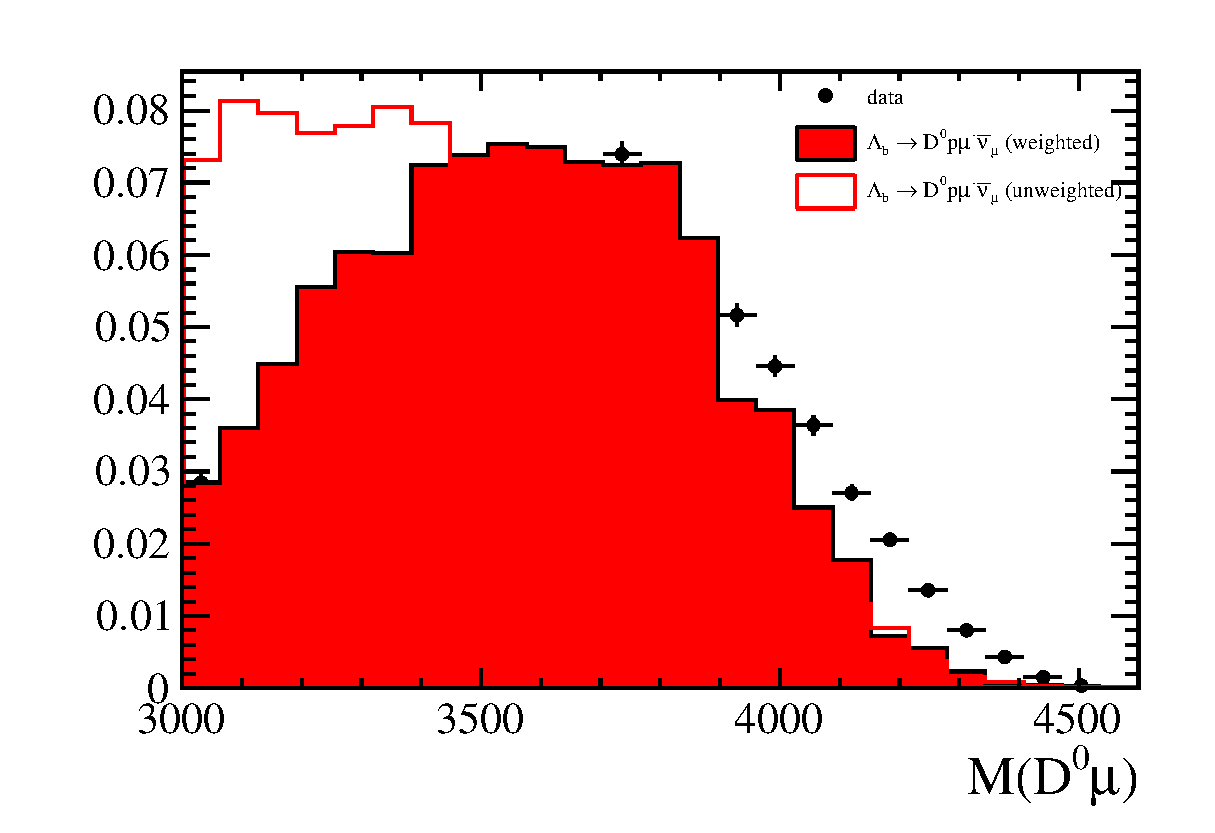
\includegraphics[width=0.49\textwidth]{LbToD0p/comparisons/3D/mD0p_mD0mu_mD0pmu/20Bins/20.0MaxWeight/B_M}
	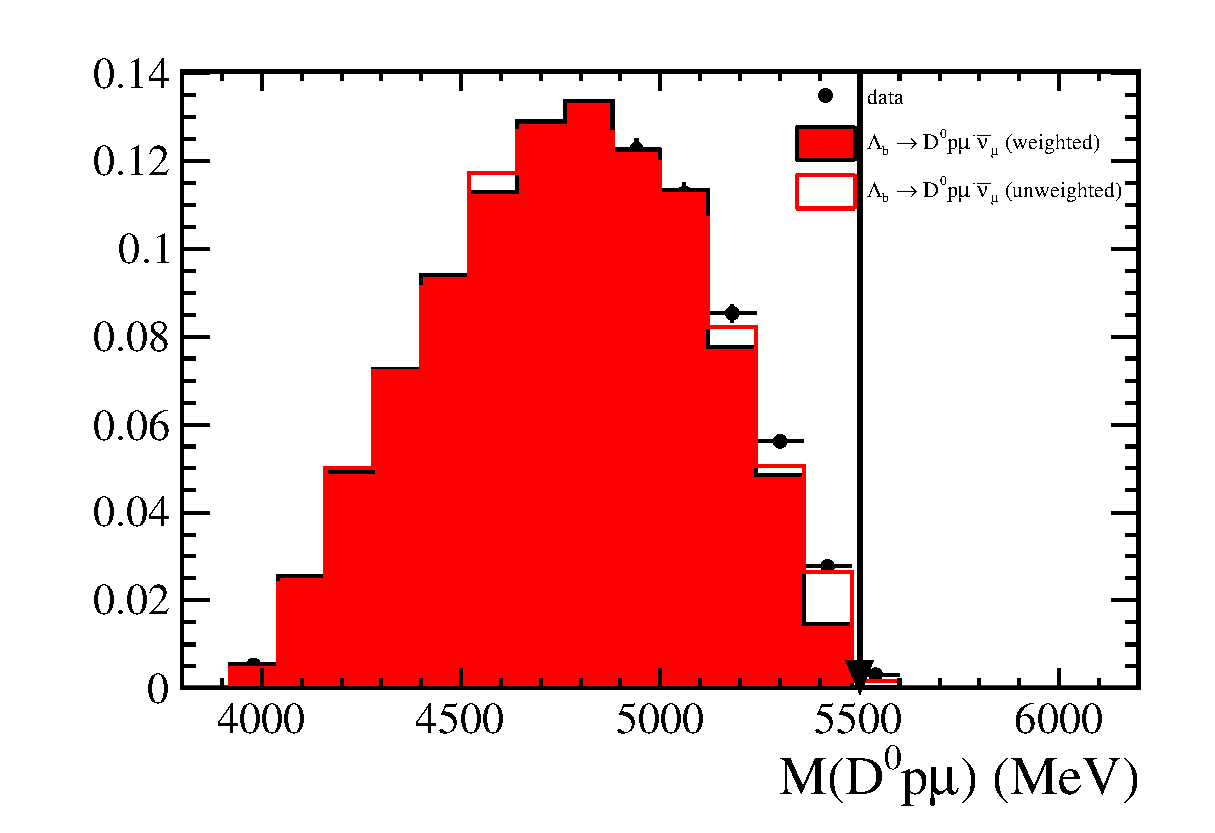
\includegraphics[width=0.49\textwidth]{LbToD0p/comparisons/3D/mD0p_mD0mu_mD0pmu/20Bins/20.0MaxWeight/Bh_M}
	\caption{Comparison of data (black points) and MonteCarlo prediction for the \LbToDpmunuX channel before (red line) and after (red shaded area) threedimensional reweighting as described in the text.}
	\label{fig:reweighting}
\end{figure}

\section{Kinematic reweighting of the \LbToDpmunuX and \LbToLcmunu channel}
The production of \Lb baryons depends strongly on their transverse momentum as figure \ref{fig:LbprodPT} from ref xxx shows. This dependence isn't well emulated by MC and has thus to be corrected. 
This was already done in ref xxx using the \decay{\Lb}{\jpsi\Dz\proton}. The weights they calculated are shown in figure \ref{fig:kinweights} and used to reweight both, \LbToDpmunuX and \LbToLcmunu channels, depending on their true \Lb transverse momentum \pt.

(\textbf{INCLUDE FIGURES FROM VUB ANALYSIS})


\section{Reweighting of the \Dz\proton signal MC}
\ref{sec:Reweight_D0p}

To reweight the \Dz\proton MC sample a threedimensional weighting in the variables
\begin{itemize}
    \item M(\Dz\proton)
    \item M(\Dz\mun)
    \item M(\Dz\proton\mun)
\end{itemize}
has been chosen. There are several reasons for this choice:
\begin{enumerate}
    \item their MC prediction is completely off from the data distribution,
    \item these variables are available as TRUE variables at generator and reconstruction level
    \item we don't cut at these variables\footnote{There exists a cut on M(\Dz\proton\mun) in this analysis to eliminate \decay{\Lb}{\Dz\proton\pim} background, but less than 0.5\% of all events have their TRUE mass above this cut. Thus, its impact on the efficiency can be neglected.}
\end{enumerate}
After the description of the reweighting and efficiency calculation process, it should become clear why these three points are important.
\begin{itemize}
    \item \textbf{Determination of the weights} \\
          There are two normalized 3D histograms drawn for both generated events (in the following called MCDecayTreeTuple or MCDTT) and events after reconstruction, applying selection cuts and the kinematic reweighting (DecayTreeTuple or DTT). 
          Both histograms have the three variables mentioned above on their axes.
          The histogram with the weights is now calculated by dividing the DTT histogram through the MCDTT histogram.
    \item \textbf{Assigning weights to the events} \\
          Now, this weight histogram is used to assign a weight to each DTT (\weight{DTT}) and MCDTT (\weight{MCDTT}) event.
          To get the correct bin in the weight histogram the true masses \Mtrue{\Dz\proton}, \Mtrue{\Dz\mun} and \Mtrue{\Dz\proton\mun} are used.
    \item \textbf{Calculation of the efficiency} \\
          The efficiency can now be calculated with
          \begin{align}
              \epsilon = \frac{\sum \weight{DTT}}{\sum \weight{MCDTT}}, \label{eq:effrew}.
          \end{align}
          To account for the loss of statistical power due to weighting, both numerator and denominator in equation \ref{eq:effrew} are multiplied by the renormalisation factor $\sum \weight{MCDTT} / \sum \weight{DTT}^2$. 
          This doesn't affect the central value of $\epsilon$ but influences the statistical error, which is calculated using binomial statistics.
\end{itemize}
It should now be clear, that we must not cut on the weighting variables, since otherwise we shouldn't now which weight has to be assigned to the MCDTT. The distribution of the masses after reweighting are also shown in figure \ref{fig:reweighting}.

\section{Generator level efficiencies}
The MC generation for the \LbToDpmunuX and \LbToLcmunu has different efficiencies. The so called ``decProdCut" requires the generated particles to be in the \lhcb acceptance during MC production. 
For example, in the case of our normalization mode \LbToLcmunu this means the \Lc and the \muon point towards \lhcb.

For signal and normalization channel we obtain the following generator level efficiencies:
\begin{align*}
    \effGenLc &= \effGenLcval \pm \effGenLcerr, \\
    \effGenDp &= \effGenDpval \pm \effGenDperr.
\end{align*}

\section{Reconstruction and selection efficiencies}
The reconstruction and selection efficiencies are calculated as described above. Whereas the \Dz\proton channel is reweighted twice (kinematic \pt(\Lb) and 3D mass reweighting) there's only the kinematic reweighting applied for the \Lc channel. The results are:
\begin{align*}
    \effSelLc &= \num[scientific-notation=true]{\effSelLcval \pm \effSelLcerr}, \\
    \effSelDp &= \num[scientific-notation=true]{\effSelDpval \pm \effSelDperr}.
\end{align*}

\section{Total efficiencies}
To summarise the values above the total efficiencies for the channels are:
\begin{align*}
    \effDp &= \effGenDp \cdot \effSelDp = \num[scientific-notation=true]{\effDpval \pm \effDperr}, \\
    \effLc &= \effGenLc \cdot \effSelLc = \num[scientific-notation=true]{\effLcval \pm \effLcerr}.
\end{align*}
For the consideration of systematics later it is sometimes more useful to consider the ratio of both efficiencies
\begin{align*}
    \frac{\effLc}{\effDp} = \effRatioval \pm \effRatioerr.
\end{align*}

  \chapter{Backgrounds}
\label{sec:Backgrounds}

The big disadvantage of semileptonic decays is that the neutrino can't be reconstructed.
At hadron colliders like the \lhc is it impossible to know the initial state, so one doesn't have enough constraints to reconstruct the full kinematic information about the decaying particle.
Being aware of these problems due to experimental setup it is clear that one can't use a well reconstructed \Lb mass peak to separate signal from background.
A main source of background is expected to be the decay \decay{\Bd/\Bp}{\Dz\mun\neumb X} where one randomly combines a proton to this decay.
Ths background is handled by the fit of the \logIP distribution.
Other sources of backgrounds and their possible impact on the obtained signal yield \NDp are discussed in the following.
For the \LbToLcmunu channel it is assumed, that all non-negligible backgrounds are accounted for due to the sidebandsubtraction and including wrong sign events as well as resonant modes components in the fit.
The discussion in this chapter thus refers completely to the \LbToDpmunuX channel.

% ====================================
% section: proton misidentification
% ====================================
\section{Proton misidentification}
A possible source of backgrounds is that one misinterprets a decay as \LbToDpmunuX since one misidentifies a final state particle.
In this analysis it is most likely that the proton is misidentified since the final state pion and kaon are reconstructed to a \Dz yielding in a nice peak and the muon leaves a clear signature in the detector due to its relatively long lifetime and low interaction with matter.
Examples for these kind of backgrounds are the decays \decay{\Bs}{\Dz\Kp\mun\neumb X} and \decay{\Bd/\Bp}{\Dz\pip\mun\neumb X}, where either the \Kp or \pip is misidentified as proton.
Though there are tight requirements on the proton identification at selection stage, the data will still be polluted by misidentified particles.
To identify the amount of misidentified protons, a slightly different data sample than the nominal one is used. 
In this sample no requirements on the proton idenfication are applied.
Except for those all other requirements are the same as described in section \ref{sec:Selection}.
However the removal of the particle identification requirements lets the data size of the sample rapidly increase.
To keep the data size acceptable a so called 5\% prescaling has been applied, i.e. only 5\% of all events are actually stored.
The decision if a particle is stored or not is made by random.
The study on misidentified backgrounds is done in three steps.

\subsection{Definition of PID particle regions - Number of particle candidates}
As a first step we define PID regions for protons, pions and kaons in the PIDK vs. PIDp plane. 
The proton region is motivated by the cuts applied in the analysis. In detail these are:
\begin{itemize}
\item proton: $\text{PIDp} - \text{PIDK} > 10.0 \text{ and } \text{PIDp} > 10.0$
\item pion: $\text{PIDp} < 10.0 \text{ and } \text{PIDK} < 0.0$
\item kaon: $\text{PIDp} - \text{PIDK} < 10.0 \text{ and } \text{PIDK} > 0.0$
\end{itemize}

Furthermore these regions and their population are visualised in figure \ref{fig:PIDregions}. From this we get the number of candidates for each particle species, in the following denoted as \Ncand{i}, with $i \in \left[\pi, \kaon, \proton\right]$. The number of candidates are
\begin{align}
    \Ncand{\pi} = \PIDNcandpionval \pm \PIDNcandpionerr, \\ 
    \Ncand{\kaon} = \PIDNcandkaonval \pm \PIDNcandkaonerr, \\ 
    \Ncand{\proton} = \PIDNcandprotonval \pm \PIDNcandprotonerr 
\end{align}

\begin{figure}[hptb]
	\centering
	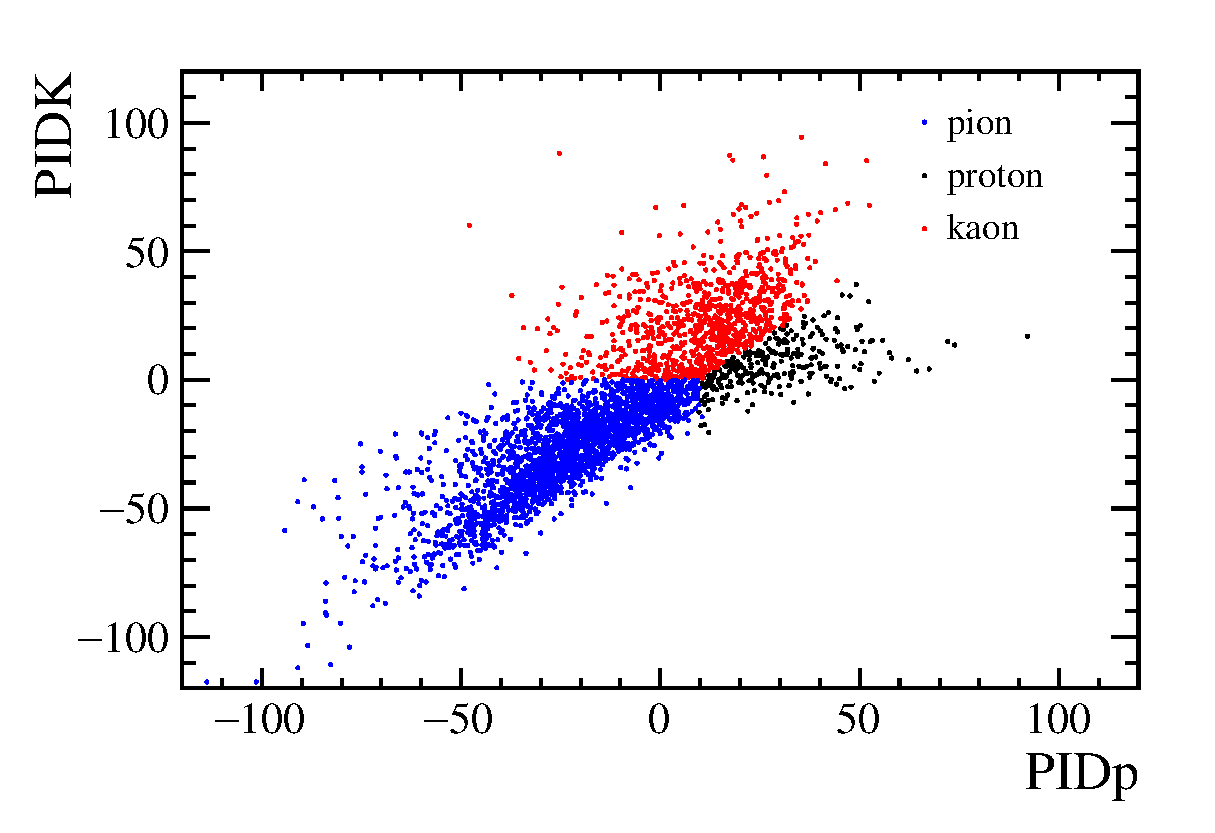
\includegraphics[width=0.49\textwidth]{LbToD0p/PID/PIDK_vs_PIDp}
	\caption{Regions for the number of particle candidates.}
	\label{fig:PIDregions}
\end{figure}


\subsubsection{Determination of ``true" candidates with PID efficiencies}
The \lhcb PIDcalib tool is used to determine the PID efficiencies, that a real proton (or kaon / pion) is identified as what we call a proton, pion or kaon according to our defined PID regions.
The PID efficiency for each of the 9 combinated is determined binwise depending on the particle momentum. The results can be seen in figure \ref{fig:PIDefficiencies}.

\begin{figure}[hptb]
	\centering
	\includegraphics[width=0.32\textwidth]{LbToD0p/PID/PID_proton}
	\includegraphics[width=0.32\textwidth]{LbToD0p/PID/PID_kaon}
	\includegraphics[width=0.32\textwidth]{LbToD0p/PID/PID_pion}
	\caption{Efficiencies determined with PIDcalib.}
	\label{fig:PIDefficiencies}
\end{figure}

To determine a final value for each efficiency, the histograms are weighted w.r.t. the kinematic distribution of our data sample. The result is:
\begin{align*}        
\begin{pmatrix}
    \effPID{\pip}{\pip}    & \effPID{\Km}{\pip}    & \effPID{\proton}{\pip} \\
    \effPID{\pip}{\Km}     & \effPID{\Km}{\Km}     & \effPID{\proton}{\Km} \\
    \effPID{\pip}{\proton} & \effPID{\Km}{\proton} & \effPID{\proton}{\proton} 
\end{pmatrix}
=
\begin{pmatrix}
0.9409 & 0.0241 & 0.1309 \\
 0.0474 & 0.9681 & 0.3798 \\
 0.0117 & 0.0077 & 0.4893
\end{pmatrix}
\end{align*}


Here, \effPID{i}{j} denotes the efficiency, that a real particle $i$ is identified as what we call $j$. 
For the following analysis, PID efficiency errors are assumed to be negligible compared to the corresponding uncertainties of the particle candidates \Ncand{i}.
With the PID efficiencies \effPID{i}{j} and the number of particle candidates \Ncand{k}, the number of ``true" particles is determined by solving the matrix equation

\begin{align*}
    \begin{pmatrix} 
        \Ncand{\pi} \\ \Ncand{\kaon} \\ \Ncand{\proton}
    \end{pmatrix}
    =
    \begin{pmatrix}
       \effPID{\pi}{\pi}     & \effPID{\kaon}{\pi}     & \effPID{\proton}{\pi} \\
       \effPID{\pi}{\kaon}   & \effPID{\kaon}{\kaon}   & \effPID{\proton}{\kaon} \\
       \effPID{\pi}{\proton} & \effPID{\kaon}{\proton} & \effPID{\proton}{\proton} 
    \end{pmatrix}
    \begin{pmatrix} 
        \Ntrue{\pi} \\ \Ntrue{\kaon} \\ \Ntrue{\proton }
    \end{pmatrix},
\end{align*}

which delivers
\begin{align}
    \Ntrue{\pi}     = \PIDNtruepionval \pm \PIDNtruepionerr, \\ 
    \Ntrue{\kaon}   = \PIDNtruekaonval \pm \PIDNtruekaonerr, \\ 
    \Ntrue{\proton} = \PIDNtrueprotonval \pm \PIDNtrueprotonerr 
\end{align}


\subsubsection{Estimate of misidentified protons}
Using the results of the previous subsections it is possible to estimate the number of misidentified protons (``true" kaons or pions identified as a proton) by multiplying the number of ``true" particles \Ntrue{i} with the PID efficiency \effPID{i}{\proton} to be identified as proton. 
\begin{align}
    N^{\pi} = \effPID{\pi}{\proton} \Ntrue{\pi}             = \PIDNtruePregionpionval \pm \PIDNtruePregionpionerr, \\  
    N^{\kaon} = \effPID{\kaon}{\proton} \Ntrue{\kaon}       = \PIDNtruePregionkaonval \pm \PIDNtruePregionkaonerr, \\ 
    N^{\proton} = \effPID{\proton}{\proton} \Ntrue{\proton} = \PIDNtruePregionprotonval \pm \PIDNtruePregionprotonerr 
\end{align}
Thus, the amount of misidentified protons is at a single-digit percent level, namely $(\misIDratioval \pm \misIDratioerr)\%$. 
Note that the absolute values can't be compared to the signal yields for both channels since this background study was done with a prescaled sample and without PID cuts.



\begin{table}
\caption{\label{tab:Backgrounds}Estimate of the residual peaking backgrounds.}
\resizebox{\textwidth}{!}{\begin{tabular}{|c|c|c|c|c|}
\hline
Mode & Estated $B/S$ & Branching fraction & Production factor & Comment \\
\hline
Signal ($\Lambda_b \rightarrow D^0 p \mu^-\nu$) & 1 & $\approx 1.5\times 10^{-3}$ & 1 & --\\
\hline
Total peaking background & 5\% & -- & -- & --\\
\hline
$\Lambda_b \rightarrow D^0 p \pi^-$ & Zero & $(5.9^{+4.0}_{-3.2})\times 10^{-4}$ & 1 & Mass veto\\
$\Lambda_b \rightarrow D^0 p \pi(\pi\pi,\pi^0)$ & 5\% & $\approx 10^{-3}$ & 1 & $\pi\rightarrow\mu$ mis-ID\\
Prompt $D^0$ & $< 10^-3$ & N/A & N/A & $\log(\mathrm{IP},D^0)$ \\ 
             &           &     &     & \& $\Lambda_b$ combination cuts\\
$B_s \rightarrow D^0 K \mu\nu X$ & $p$-misid & $\approx 6\times 10^{-3}$  & 0.5 & $p$-mis-ID\\
                                 &          & (resonant part)             &        \\
\hline
\end{tabular}}
\end{table}


The following backgrounds to the the $\Lambda_b^0 \rightarrow D^0 p \mu \nu X$ sample are considered:


\begin{itemize}
\item {\bf Prompt $D^{0}$}\\
The prompt $D^0$ cross section exceeds that of $\Lambda_b^0$ production by a factor of twenty or so.
The background from prompt charm production is typically measured to be {\bf a few percent} in studies of semileptonic $b$ decays.
Suggest to plot the distribution of the $\log(\mathrm{IP})$ of the $D^0$, which should reveal the prompt component.
This should be clearer in candidates with a wrong sign muon, or wrong sign proton, or both.
By requring a large $\log(\mathrm{IP})$ of the $D^0$, we should be able to eliminate this background althogether.
\item {\bf $B_s^{0} \rightarrow D^0 K \mu \nu X$}\\
Where the kaon is mis-identified as a proton. The mis-id rate should be a few percent, given
our tight proton PID requirements. And $f_{\Lambda_b}/f_s \sim 2$.
We should be able to estimate this contribution quite precisely just from the numbers in an early LHCb
study with 2010 data~\cite{Aaij:2011ju}.
\item {\bf $B^{0,+} \rightarrow D^0 \pi^+ \mu \nu X$}\\
Where the pion is mis-identified as a proton. The mis-id rate should be very small,
and these decays are quite well understood.
\item {\bf $B^{0,+} \rightarrow D^0 \mu \nu X$ plus a proton from the PV or other $b$}\\
This component is subtracted in our fit to the $\log(\mathrm{IP})$ of the proton w.r.t. the $D^0\mu$ vertex.
\item {\bf $\Lambda_b^0 \rightarrow D^0 p \pi X$}\\
      Where the pion is mis-identified as a muon. 
      The branching fraction of this decay has been measured to be less than $10^{-3}$. It sits in a very narrow region of $\Dz\proton\mun$ invariant mass peaking at the \Lb mass. 
      This background is eliminated by a cut on the \Dz\proton\mun mass as can be seen in figure \ref{fig:plot_D0pmuMass}.
\item {\bf \decay{\Lb}{\Dz\proton 3\pi}} \\
      The branching fraction should be similar to \decay{\Lb}{\Dz\proton\pi X}, i.e. of order $10^{-4}$. 
      The amount should decrease with increasing muon identification. 
      Figure \ref{fig:plot_D0pmuMass_vs_muPIDmu} shows a 2D plot of the \Dz\proton\muon mass versus the particle identification variable PIDmu of the muon. 
      Backgrounds coming from a \Lb decay into 3 pions should cluster at low PIDmu, where it is rather probable that a muon is misidentified than in the high PIDmu region.
\item {\bf $\Lambda_b^0 \rightarrow D \Lambda_c$}\\
      This decay hasn't been measured but it should have a branching ratio of around $10^{-2}$, similar to $B \rightarrow D D_s$.
      If the $\Lambda_c$ decays to $pK\pi$, then we get another $4 \times 10^{-2}$ and we need to get the muon from somewhere else, 
      or it has to be from $K \rightarrow \mu$ mis-id. 
      The vertex quality will be somewhat spoilt by the $\Lambda_c$ flight.
      So this should be a sub-percent-level background.
      One could also get $\Lambda_c N^* \mu \nu$, where we get the muon and proton without any mis-id?
\item {\bf $\Lambda_b^0 \rightarrow D^0 D^- p$}\\
This decay hasn't been measured but it should be similar to $B \rightarrow DDK$ at a few times $10^{-3}$.
The inclusive $D^- \rightarrow \mu^-X$ branching fraction is about $10^{-2}$.
This should still be a percent level background.
\item {\bf prompt \LcResI or \LcResII decay with an \mun from somewhere else} \\
This background should be reduced by requiring the \LcResI resp. \LcResII vertex to be well separated from the PV.
\item \textbf{ \decay{\SigmabRes}{\Lb \pi}}, where the pion isn't reconstructed.
\end{itemize}

\begin{figure}[hptb]
	\centering
	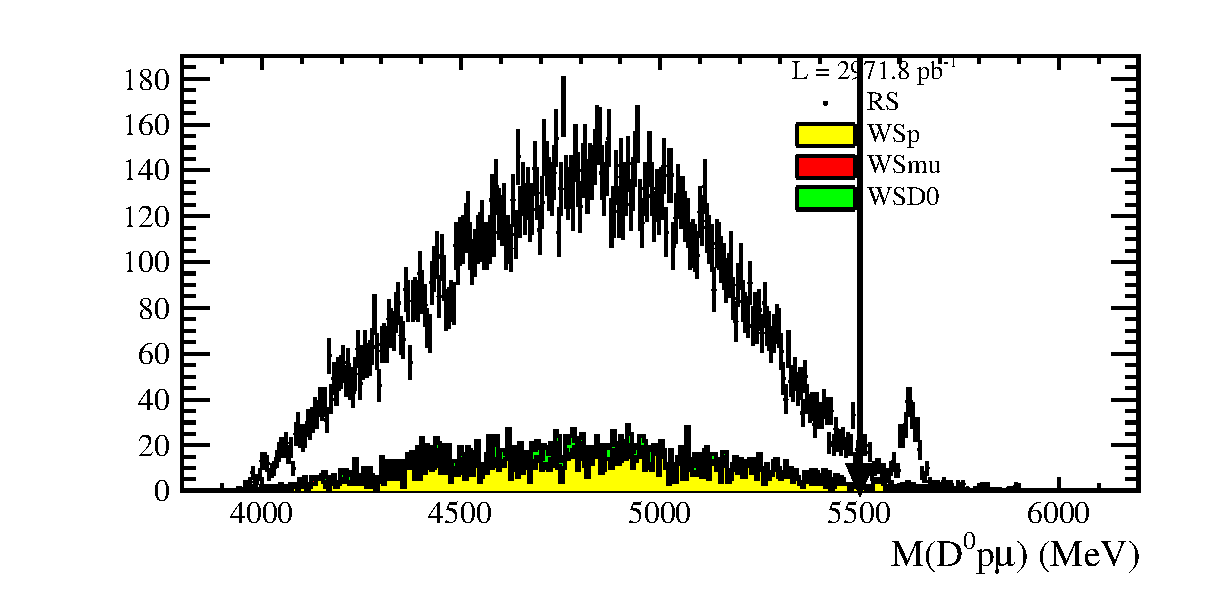
\includegraphics[width=0.49\textwidth]{LbToD0p/plots/data/Bh_M}
	\caption{Invariant \Dz\proton\mun mass. The arrow indicates the cut applied in this analysis. The peak at \Lb mass ($\approx 5620 \mev$) comes from the decay \decay{\Lb}{\Dz\proton\pi} where the pion is misidentified as muon.}
	\label{fig:plot_D0pmuMass}
\end{figure}

\begin{figure}[hptb]
	\centering
	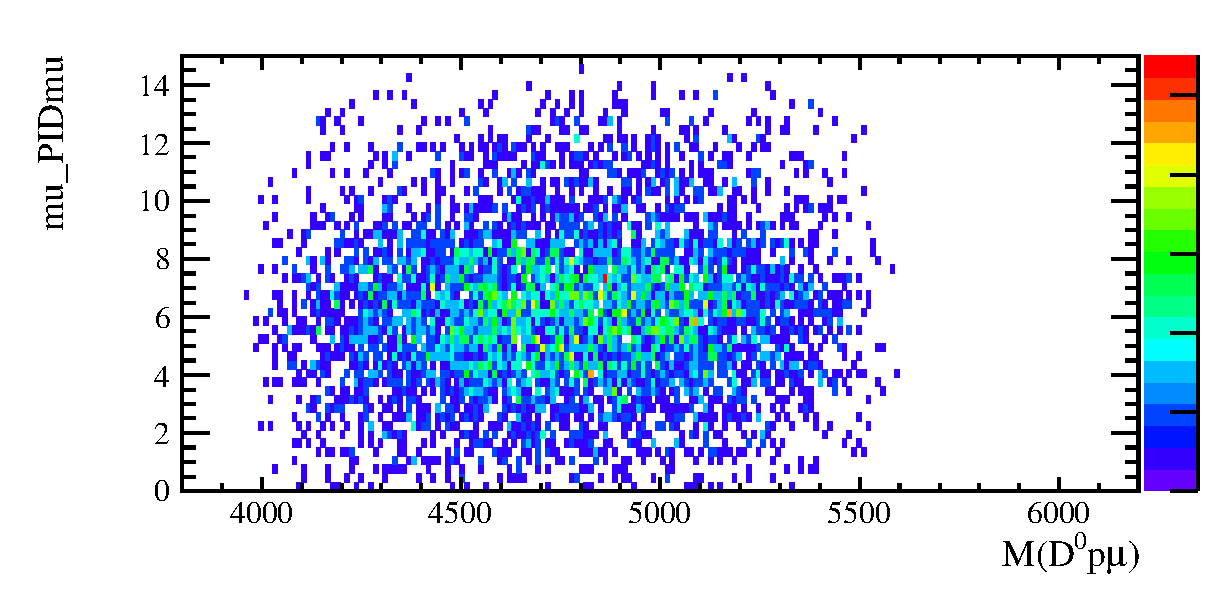
\includegraphics[width=0.49\textwidth]{LbToD0p/plots/data/Bh_M_vs_mu_PIDmu_RS}
	\caption{Invariant \Dz\proton\mun mass versus PIDmu of the muon. No structures tending to low PIDmu can be seen.}
	\label{fig:plot_D0pmuMass_vs_muPIDmu}
\end{figure}


  \chapter{Systematics}
\label{sec:Systematics}



  \section{Checks concerning the enhancement at low \Dz\proton mass}
\label{sec:Structure}

In section \ref{sec:Signalfit} it has been stated that the fit of the \Dz\proton mass spectrum needs an additional component to parametrize an enhancement at low \Dz\proton masses right after threshold.
An appropriate model for that enhancement has seemed to be parametrized like the two \LcResI and \LcResII resonances.
This doesn't mean at all that there is really an additional resonance seen.
There might be a lot of other reasons, e.g.:
\begin{itemize}
    \item Detector threshold / acceptance effects,
    \item Low mass behaviour induced by some selection requirements,
    \item Feed-down from partially reconstructed decays,
    \item Threshold enhancement due to wide resonances below \Dz\proton mass threshold.
\end{itemize}
In this chapter several checks are done to either explain the origin of this enhancement or rule out some of the ideas.
It should be mentioned, that there won't be a final answer to that question.
If this was really something new, it would be really hard to prove it with a semileptonic decay channel.
There is currently another \lhcb analysis on the exclusive hadronic decay \decay{\Lb}{\Dz\proton\pim} running, seeing a similar enhancement at low \Dz\proton mass.
This channel enables to study the enhancement with more methods for instance with an amplitude analysis making it possible to tell more about it.

\subsection{Detector threshold / acceptance effect}
One possible explanation of the enhancement might be a simple threshold respectively acceptance effect of the detector or caused by the application of some selection requirements.
To clarify this possibility and estimate the effects of the detector and the selection requirements the simulation samples at generator level and at reconstruction level are used.
Figure \ref{fig:detector_cut_effect} shows the invariant \Dz\proton mass at different stages in generation and reconstruction.
The green distribution shows the \Dz\proton mass at generation level, i.e. there's no simulation of the detector or any reconstruction applied here.
In blue one sees the \Dz\proton mass after the simulation of the detector and in red the mass after reconstruction and selection.
For comparison the measured data distribution is shown in black as well.
In this case always the so called ``true" masses are plotted, i.e. there are no influences of the detector resolution in these distributions.
This figure shows that the distribution behaves similar and there isn't any significant acceptance effect arising neither due to the detector itself nor due to the reconstruction and selection process. 
Thus, the enhancement can't be caused by such an effect.
\begin{figure}[hptb]
	\centering
	\includegraphics[width=0.49\textwidth]{LbToD0p/structure/detector_cut_effect}
	\caption{Simulated (true) invariant \Dz\proton mass at different stages, namely after generation (green), detector simulation (blue) and reconstruction and selection (red). The black line shows the measured data.}
	\label{fig:detector_cut_effect}
\end{figure}

Excluded to get any structure from acceptance effects a closer look at the \Dz\proton mass threshold reveals some kind of an ``S-shaped" curvature in the ascending part.
This can be better seen with a zoom into this region as shown in figure \ref{fig:mD0p_zoom}.
\begin{figure}[hptb]
	\centering
	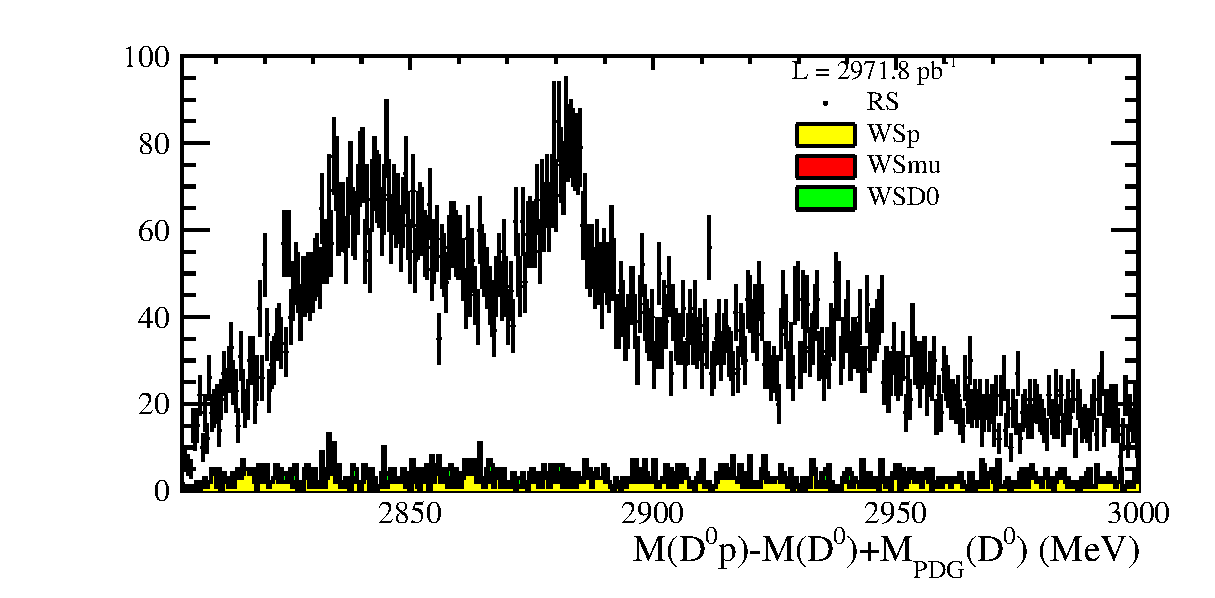
\includegraphics[width=0.49\textwidth]{LbToD0p/plots/data/Bh_DELTA_MASS_zoom}
	\caption{Zoom into the low \Dz\proton mass region.}
	\label{fig:mD0p_zoom}
\end{figure}

Due to this curvature the fit isn't able to describe the low \Dz\proton mass region only with a nonresonant component but rather prefers to have an additional component. 
At this point it should be mentioned that there are other analyses seeing a similar behaviour in this \Dz\proton mass region.

First of all, there is a study by \babar on the \Dz\proton final state (see fig. \ref{fig:Babar_D0p} aiming to measure the \LcResI and \LcResII resonance (and in the latter case to even observe it).
While discussing their systematics, they're wondering if this much less pronounced (compared to this analysis) bump at roughly 2840\mev might change their results by adding an additional resonance component to their fit. 
Since the impact isn't that large they just include the deviations in their systematics, unfortunately without trying to understand the origin of this bump \cite{Babar_D0p}.
\begin{figure}[hptb]
	\centering
	\includegraphics[width=0.49\textwidth]{Babar_D0p}
	\caption{\babar study on the \Dz\proton final state. They suspect to see a structure similar to the enhancement in the current analysis and fit it in c) with an additional resonance component for their systematic studies. Figure taken from \cite{Babar_D0p}.}
	\label{fig:Babar_D0p}
\end{figure}

Furthermore, there are two more running \lhcb studies on either prompt \Dz\proton events and on the hadronic \decay{\Lb}{\Dz\proton\pim} decay.
It can be disclosed that they are struggling with the same problem, seeing a pronounced enhancement around 2840\mev without being (currently) able to explain it.
However, since there doesn't exist any approved material, nothing of their plots can be shown in this thesis.

Being seen in different channels and analysis substantiates the assumption, that there is a physical reason for the enhancement.

\subsection{Threshold enhancement from other resonances}


\subsection{Further ideas}
\begin{itemize}
    \item The unknown structure in the low mass region of the \Dz\proton spectrum could have its origin in the decay \decay{\SigmacpRes{(2880)}}{\Dz\proton}, which is kinematically exactly at threshold ($M(\proton)+M(\Dz)=2802\mev$).  
          The \SigmacpRes{(2880)} in turn could be part of the decay \decay{\SigmabpRes}{\SigmacpRes{(2880)}\mun\neumb}. 
          Another possibility would be \decay{\Lb}{\SigmacpRes{(2880)}\mun\neumb} which should be allowed by Feynman rules but might be forbidden by isospin violation since $I(\Lb) = 0$ and $I(\SigmacpRes{(2880)}) = 1$. 
          On the other hand weak decays don't respect isospin conservation.
          However, this resonance should lead to a threshold enhancement causing a steep smooth ascent at mass threshold and not having this ``S-curvature"
    \item The peak could come from a resonance decaying into an excited \Dstar(2007)\proton with \Dstar(2007) \to \Dz\pion where the \pion isn't reconstructed.
          The \LcResI is too light to decay in \Dstar(2007)\proton and even the \LcResII is slightly below the \Dstar(2007)\proton mass threshold of 2945 \mev. 
          Maybe there is a heavier resonance proceeding via this decay, maybe a partially reconstructed decay of a \Sigmacp.
    \item Direct product of an excited \Lc or \Sigmacp state. The muon should then randomly combined???
    \item 
    \item ...
\end{itemize}



  \chapter{Results}
\label{sec:Results}
This chapter summarises all the ingredients needed for the calculation of the relative branching ratio \R.
As a reminder, the relative branching ratio of the decays \LbToDpmunuX and \LbToLcmunu is calculated by:
\begin{align}
	\R =
	\frac{\BR(\decay{\Lb}{\Dz\proton \mun \neumb X})}{\BR(\decay{\Lb}{\Lc \mun\neumb})}
	 = 
	 \frac{N_{\Dz\proton}}{N_{\Lc}}  
	 \cdot \frac{\epsilon_{\Lc}}{\epsilon_{\Dz\proton}}
	 \cdot \frac{\BR(\decay{\Lc}{p \Km \pip})}{\BR(\decay{\Dz}{\Km\pip})}.
\end{align}

Concerning the signal yield \NDp of the \LbToDpmunuX channel, not all backgrounds could be separated in the signal fit, since it is only able to separate random background.
In section \ref{sec:Backgrounds} additional background contributions like fake protons etc. have been discussed and a background yield \NBgdDp has been assigned.
Thus the final calculation of R is modified to
\begin{align}
	\R =
	 \frac{N_{\Dz\proton}-\NBgdDp}{N_{\Lc}}  
	 \cdot \frac{\epsilon_{\Lc}}{\epsilon_{\Dz\proton}}
	 \cdot \frac{\BR(\decay{\Lc}{p \Km \pip})}{\BR(\decay{\Dz}{\Km\pip})}. \label{eq:R_mod}
\end{align}
Note that for the normalisation fit and the determination of \NLc it is assumed, that all non-negligible backgrounds are considered in the fit.
The efficiency ratio \effRatio has been determined by the use of simulation samples.
These had to be reweighted to better emulate the data distribution.

 
\begin{table}[h]
    \centering
    \caption{Final results needed for the calculation of \R according to equation (\ref{eq:R}). The errors correspond to the statistical (first) and systematic (second) precision.}
    \label{tab:table_finalresults.tex}
    $\begin{array}{lr@{\pm}r@{\pm}l}
    \hline
    \text{Variable} & \multicolumn{3}{c}{\text{Value}} \\
    \hline
\multicolumn{4}{l}{\text{\textbf{Signal yields}}} \\
\NDp&(2.29 & 0.02 & 0.07) \cdot 10^{4}\\
\NLc&(1.55 & 0.01 & 0.00) \cdot 10^{6}\\
\multicolumn{4}{l}{\text{\textbf{Backgrounds}}} \\
\NBgdDp&(2.75 & 0.03 & 0.00) \cdot 10^{3}\\
\multicolumn{4}{l}{\text{\textbf{Branching ratios}}} \\
\DBFDp&(3.88 & 0.00 & 0.05) \cdot 10^{-2}\\
\DBFLc&(6.84 & 0.00 & 0.24) \cdot 10^{-2}\\
\multicolumn{4}{l}{\text{\textbf{Efficiencies}}} \\
\effDp&(1.79 & 0.36 & 0.11) \cdot 10^{-3}\\
\effLc&(1.35 & 0.07 & 0.00) \cdot 10^{-3}\\
\frac{\effLc}{\effDp}&(7.50 & 1.60 & 0.50) \cdot 10^{-1}\\

    \hline
    \end{array}$
\end{table}

An overview of all important observables can be found in Table \ref{tab:table_finalresults}.
With these values the relative branching ratio \R gets
\begin{align*}
    \R = \Rval \pm \Rerr\stat \pm \Rsysterr\syst.
\end{align*}
The statistical error dominates compared to the systematic uncertainty.
The main contribution comes from the statistical uncertainty on the efficiency.
Above all the simulation sample at generator level includes only little statistics.

  \chapter{Conclusion}
\label{sec:Conclusion}
This thesis presents the first branching ratio measurement of the semileptonic decay \LbToDpmunuX in form of a relative branching fraction ratio $\R := \frac{\BR(\LbToDpmunuX)}{\BR(\LbToLcmunu)}$.
The analysed data has been collected by the \lhcb experiment in the years 2011 and 2012 corresponding to an integrated luminosity of \intlum{3\invfb}.
The determination of \R requires in principle four quantities: the signal yields of the channels \LbToDpmunuX and \LbToLcmunu as well as the corresponding reconstruction and selection efficiencies.
As only events with the daughter decays \DToKpi and \LcTopKpi are reconstructed \R has to be corrected for their respective branching ratios.
These values are taken from other experiments.

Due to the semileptonic nature of signal and normalisation channel, it has not been possible to reconstruct the \Lb mass to get the signal yields.
The signal yield of the decay \LbToDpmunuX has been determined with a two-dimensional fit of the \Dz\proton mass and the \logIP distribution.
Being a measure of how well the \proton makes a vertex with the \Dz\mun candidate, \logIP enables to distinguish between signal and background from randomly combined protons.
This is very helpful to disentangle the nonresonant \LbToDpmunuX decays from background in the \Dz\proton mass spectrum.
The fit yields in total $(\NDpvalscient \pm \NDperrscient)\cdot 10^{\NDpexpscient}$ signal candidates.
However, the fit does not prevent that other backgrounds than randomly combined protons leak into the signal.
It has been shown that the main backgrounds are either fake protons or muons, i.e. decays, that mimic to be \LbToDpmunuX since one of the particles is misidentified as proton or muon.
The leakage of backgrounds into the signal yield has been estimated as $(\NDpBKGratioval \pm \NDpBKGratioerr)\%$.

An anomalous enhancement has been observed in the invariant \Dz\proton mass spectrum at a mass of about 2840 \mev.
Different attempts to explain its origin have been made without a final solution.
As it currently seems that this enhancement is anyhow part of an inclusive \LbToDpmunuX decay, its yield is counted as signal.

For the reference channel \LbToLcmunu, he problem of backgrounds has not been a randomly combined proton but rather that excited \Lcstar states pollute the data.
These decays could be identified by their to lower values shifted corrected \Lb mass.
The fit of the corrected mass is based on simulation templates and yields $(\NLcvalscient \pm \NLcerrscient)\cdot 10^{\NLcexpscient}$.
It is assumed that all relevant backgrounds are already subtracted before or in the fit.

For the determination of the reconstruction and selection efficiencies the necessary simulations had to be reweighted, especially the simulation of the decay \LbToDpmunuX.
The ratio of both efficiencies has been determined to be $\frac{\effLc}{\effDp} = \effRatioval \pm \effRatioerr$.

This leads to the final result of the relative branching ratio
\begin{align*}
    \R = \Rval \pm \Rerr\stat \pm \Rsysterr\syst.
\end{align*}
The statistical uncertainties dominates.
This is not a problem of too few recorded events but rather the \LbToDpmunuX simulation at generator level does not contain enough data.
Thus, the statistiscal error on the efficiencies is quite large, above all the generator level efficiency \effGenDp of the \LbToDpmunuX signal channel amounts to about $20\%$.
The biggest contribution to the systematic uncertainties comes from the reweighting process.
It will certainly become more accurate if a proper theoretical physics description is available.
Unfortunately, the theoretical interest in these kind of decays is rather poor.
There is no prediction, to be compared with the obtained result.
Since this is the first measurement of \BR(\LbToDpmunuX) anyway, there are no other experimental results for comparison either.

What is left is the question of the origin of the enhancement at low \Dz\proton mass.
There are currently different analyses running at \lhcb seeing a similar behaviour in the invariant \Dz\proton mass.
Hopefully, an explanation can be found with combined efforts.
Since this enhancement is overlapping with the \LcResI resonance in the \Dz\proton spectrum, the obtained masses and widths of the \LcResI and \LcResII are only preliminary.
These results are clearly depending on the parametrisation of the enhancement.
Thus, the obtained properties of the \LcResI and \LcResII are not quoted here again.
To get reliable results here, it has to be clear, what the enhancement's nature is and how large the impact of the \LcRes{(2765)} and \SigmacpRes{(2800)} to the invariant \Dz\proton mass at threshold is.



  \begin{appendix}
    \chapter{Mass resolution}
\label{app:Massresolution}
Figure \ref{fig:massresolution_all} shows the fits to all bins of \Dz\proton mass for the determination of the mass resolution.
The whole method and prodecure is described in Section \ref{sec:Massresolution}.
\begin{figure}[hptb]
    \centering
	\includegraphics[width=0.32\textwidth]{LbToD0p/massresolution/massresolution_00}
	\includegraphics[width=0.32\textwidth]{LbToD0p/massresolution/massresolution_01}
	\includegraphics[width=0.32\textwidth]{LbToD0p/massresolution/massresolution_02} \\
	\includegraphics[width=0.32\textwidth]{LbToD0p/massresolution/massresolution_03}
	\includegraphics[width=0.32\textwidth]{LbToD0p/massresolution/massresolution_04}
	\includegraphics[width=0.32\textwidth]{LbToD0p/massresolution/massresolution_05} \\
	\includegraphics[width=0.32\textwidth]{LbToD0p/massresolution/massresolution_06}
	\includegraphics[width=0.32\textwidth]{LbToD0p/massresolution/massresolution_07}
	\caption{Fit of a double Gaussian to the difference between generated and reconstructed \Dz\proton mass (simulation sample) in different bins of true \Dz\proton mass. The width of distributions corresponds to the mass resolution for the respective bin.}
    \label{fig:massresolution_all}
\end{figure}

\chapter{Reweighting of \LbToDpmunuX decay simulation}
\label{app:Reweight_D0p}
Figure \ref{fig:reweight_D0p_app} shows several more comparisons of data and simulation before and after reweighting.
More on the reweighting process can be found in Section \ref{sec:Reweight_D0p}.
\begin{figure}[hptb]
    \centering
	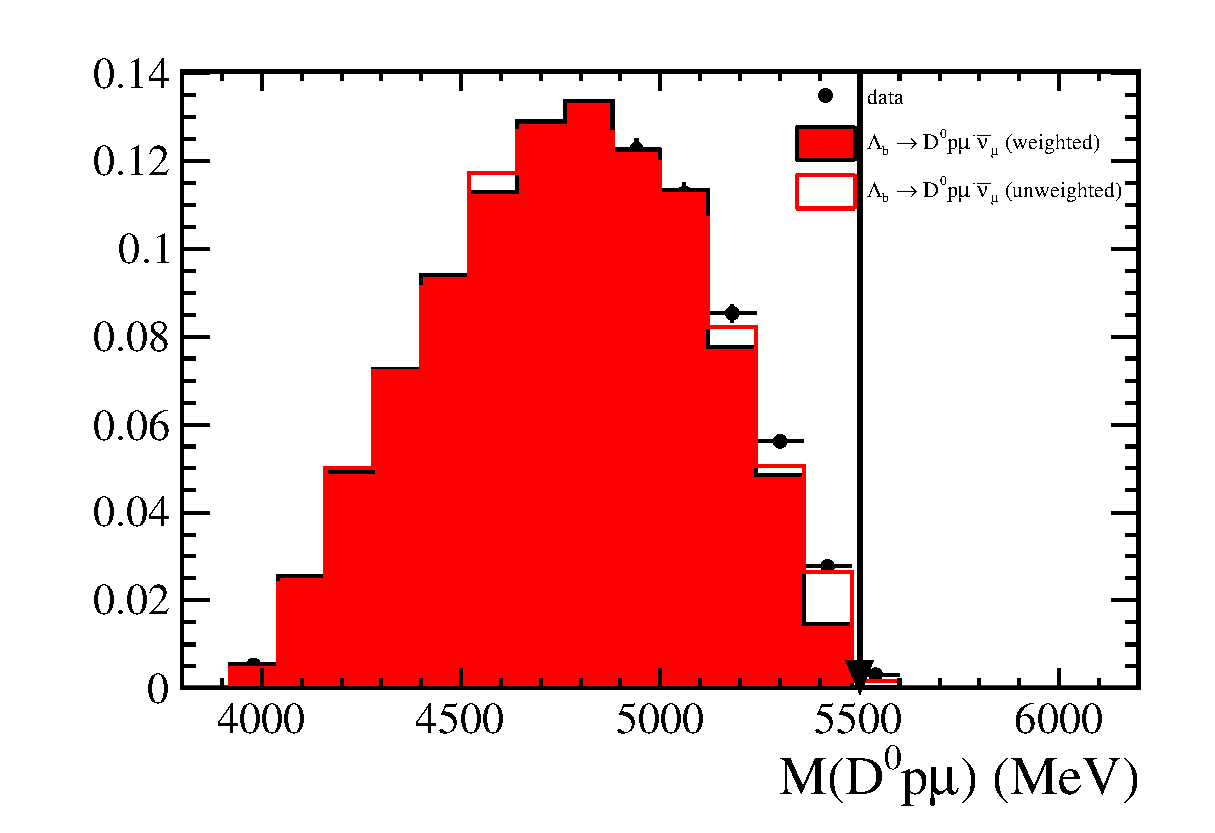
\includegraphics[width=0.32\textwidth]{LbToD0p/comparisons/3D/mD0p_mD0mu_mD0pmu/20Bins/20.0MaxWeight/Bh_M}
	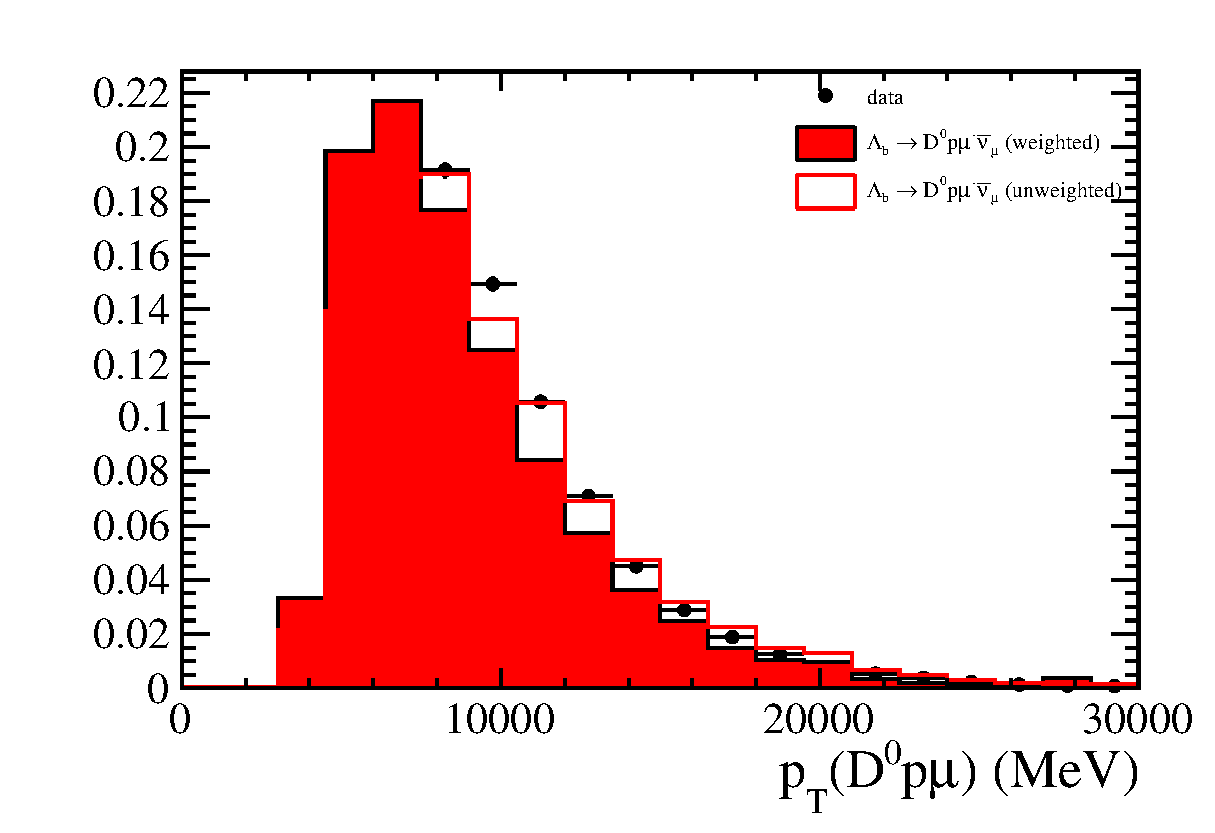
\includegraphics[width=0.32\textwidth]{LbToD0p/comparisons/3D/mD0p_mD0mu_mD0pmu/20Bins/20.0MaxWeight/Bh_PT}
	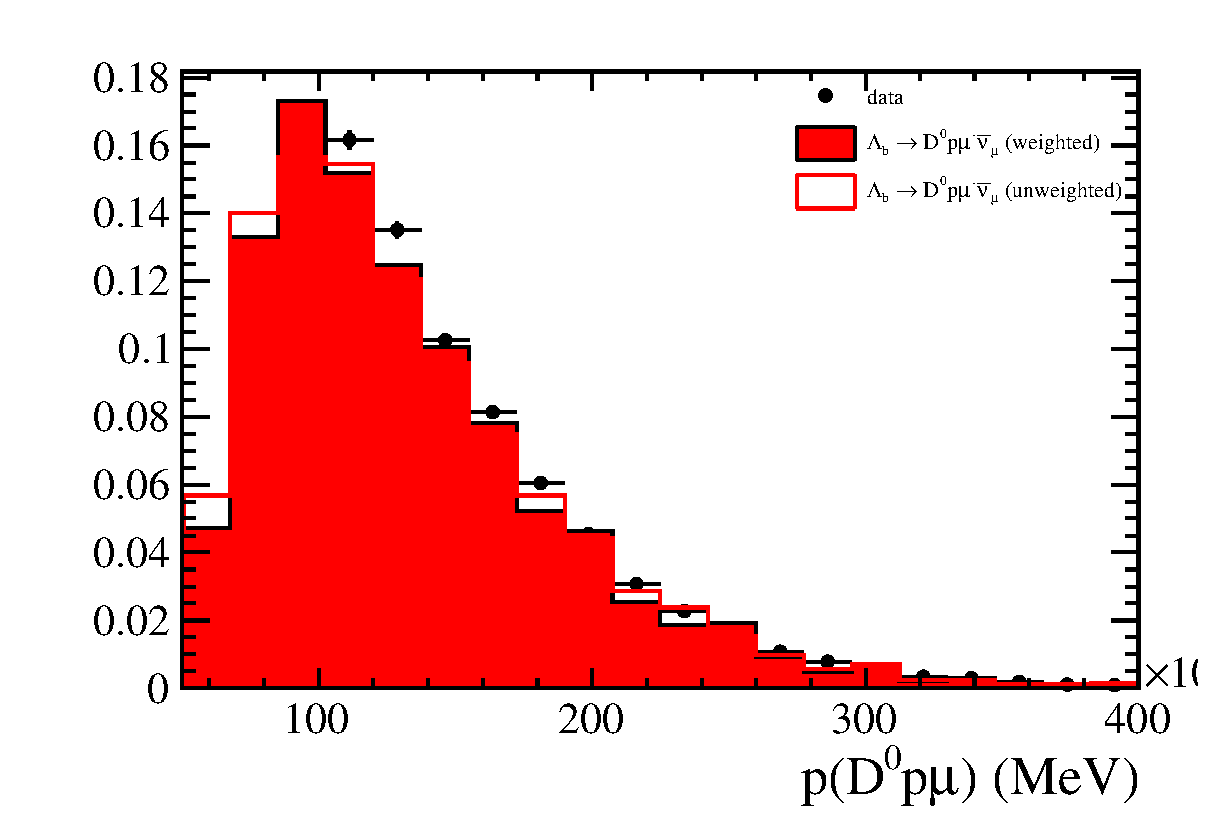
\includegraphics[width=0.32\textwidth]{LbToD0p/comparisons/3D/mD0p_mD0mu_mD0pmu/20Bins/20.0MaxWeight/Bh_P}          \\
	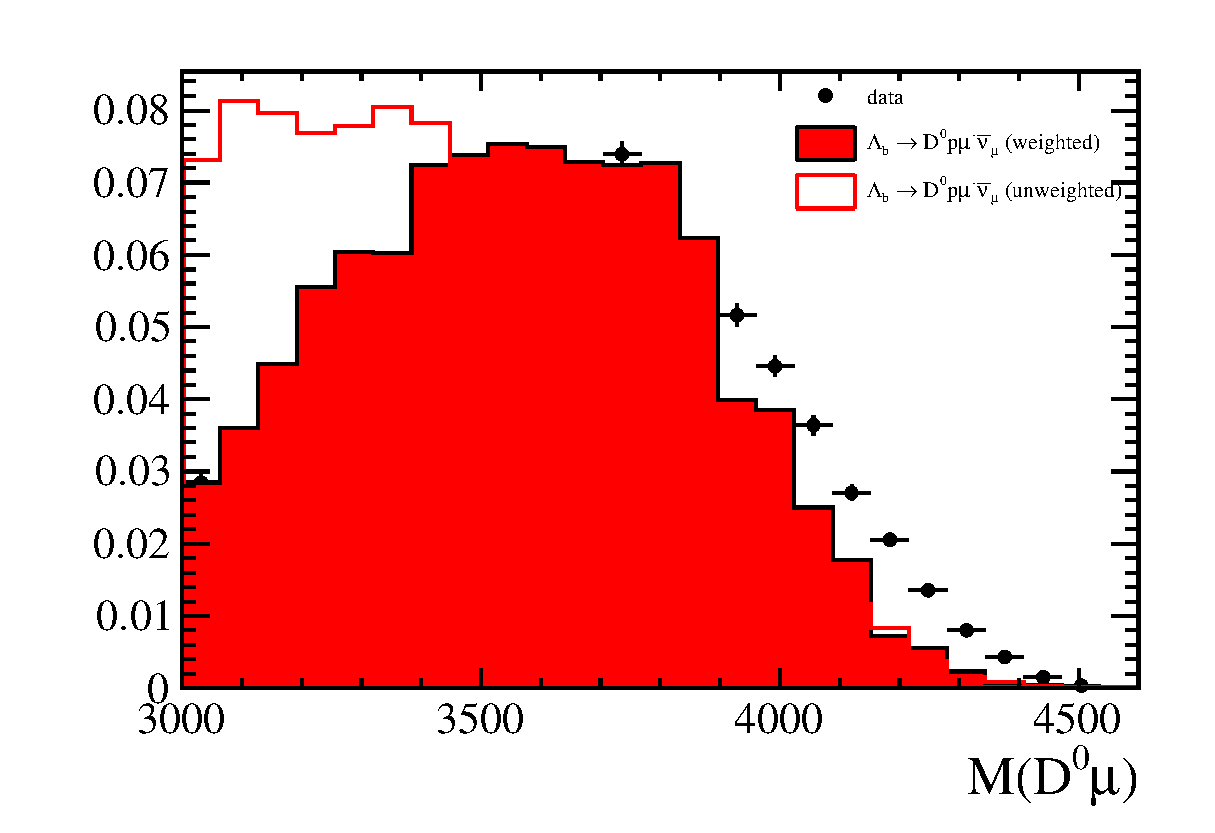
\includegraphics[width=0.32\textwidth]{LbToD0p/comparisons/3D/mD0p_mD0mu_mD0pmu/20Bins/20.0MaxWeight/B_M}           
	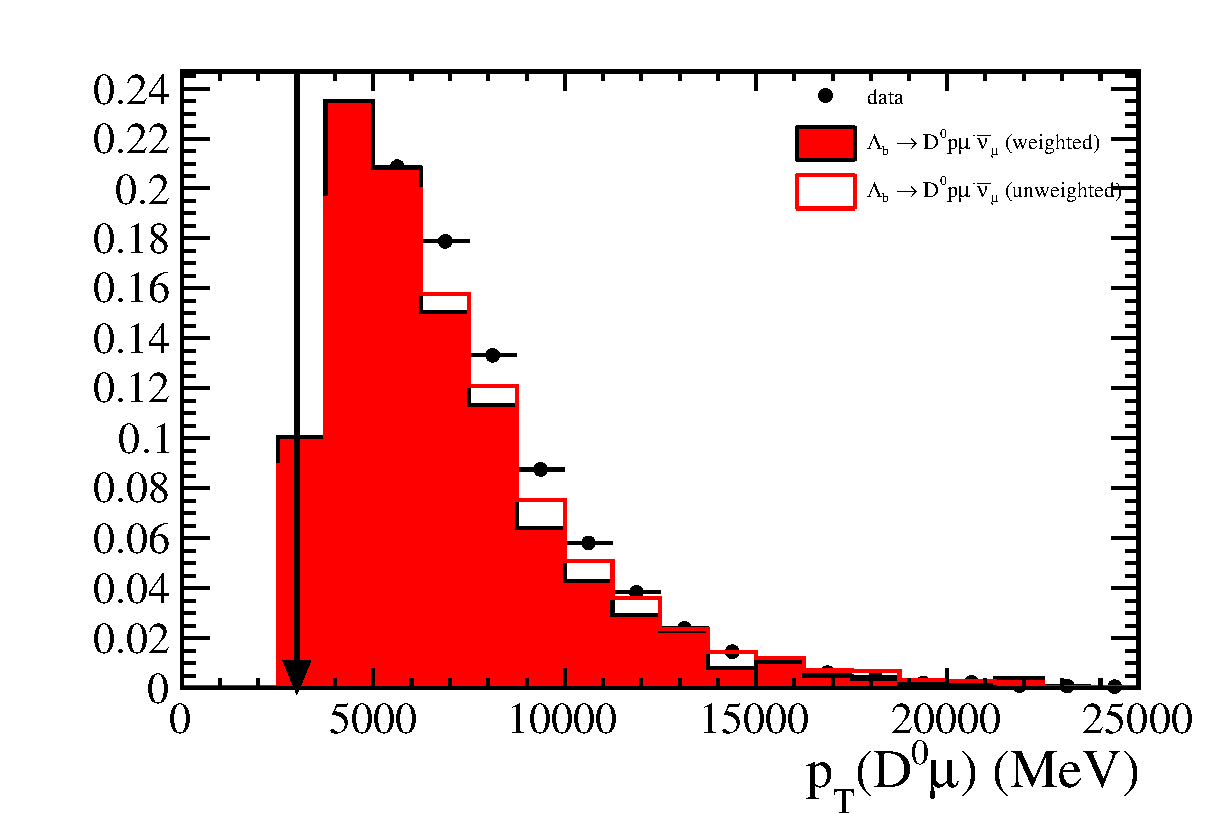
\includegraphics[width=0.32\textwidth]{LbToD0p/comparisons/3D/mD0p_mD0mu_mD0pmu/20Bins/20.0MaxWeight/B_PT}
	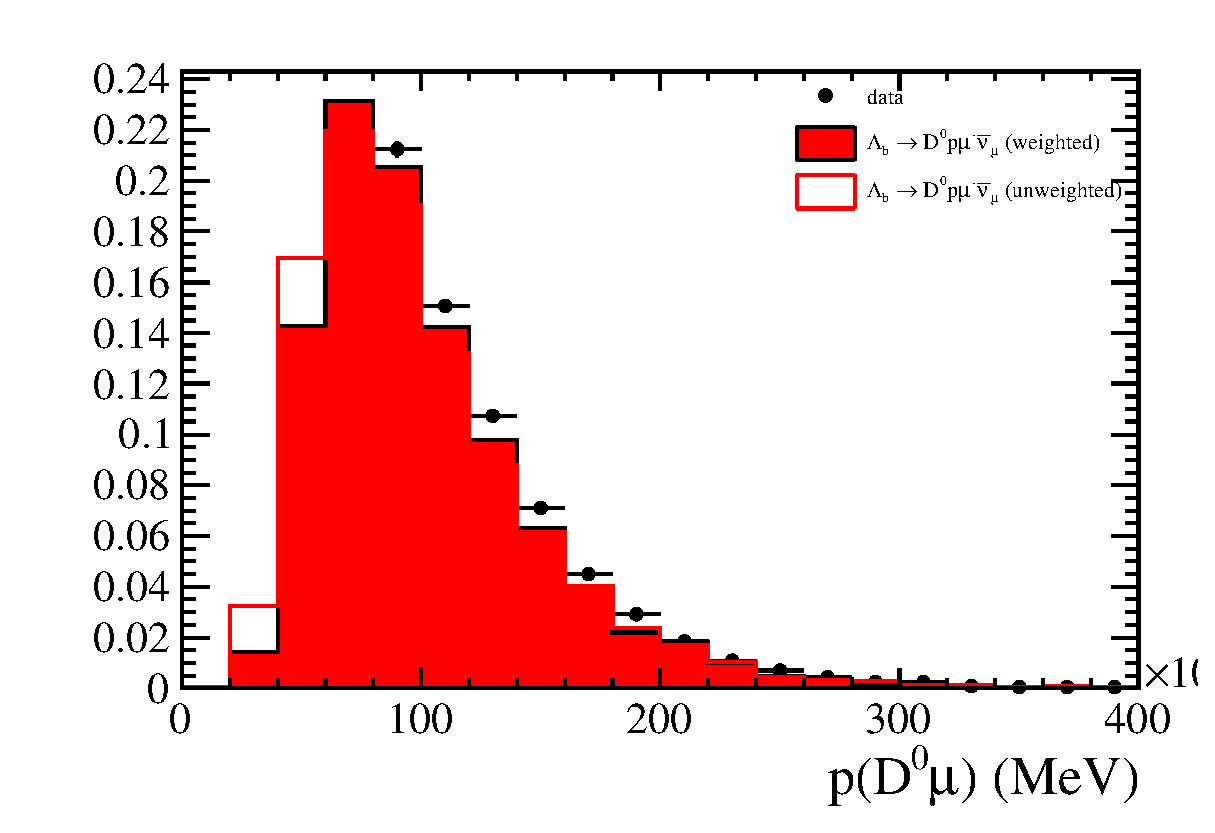
\includegraphics[width=0.32\textwidth]{LbToD0p/comparisons/3D/mD0p_mD0mu_mD0pmu/20Bins/20.0MaxWeight/B_P}           \\
    \includegraphics[width=0.32\textwidth]{LbToD0p/comparisons/3D/mD0p_mD0mu_mD0pmu/20Bins/20.0MaxWeight/Bh_DELTA_MASS}
	\includegraphics[width=0.32\textwidth]{LbToD0p/comparisons/3D/mD0p_mD0mu_mD0pmu/20Bins/20.0MaxWeight/D0_PT}
	\includegraphics[width=0.32\textwidth]{LbToD0p/comparisons/3D/mD0p_mD0mu_mD0pmu/20Bins/20.0MaxWeight/D0_P}          \\
    \includegraphics[width=0.32\textwidth]{LbToD0p/comparisons/3D/mD0p_mD0mu_mD0pmu/20Bins/20.0MaxWeight/logIP}
	\includegraphics[width=0.32\textwidth]{LbToD0p/comparisons/3D/mD0p_mD0mu_mD0pmu/20Bins/20.0MaxWeight/h_P}
	\includegraphics[width=0.32\textwidth]{LbToD0p/comparisons/3D/mD0p_mD0mu_mD0pmu/20Bins/20.0MaxWeight/h_PT}
	\caption{Comparison of data (black points) and simulation for the \LbToDpmunuX channel before (red line) and after (red shaded area) threedimensional reweighting as described in Section \ref{sec:Reweight_D0p}.}
    \label{fig:reweight_D0p_app}
\end{figure}

\chapter{Reweighting and comparison of the \LbToLcmunu candidates}
\label{app:Reweight_Lc}
Except for the kinematic \pt(\Lb) reweighting, no additional reweighting is applied as for \LbToDpmunu. 
However, the data is polluted by two decays into excited states, \decay{\Lb}{\LcstarRes{(2593)}\mun\neumb} and \decay{\Lb}{\LcstarRes{(2625)}\neumb}. 
Thus, Figure \ref{fig:reweight_Lc_app} shows a comparison of side bandsubtracted data and the sum of the three different channels.
They are summed up according to the yields obtained by the fit to the corrected \Lb mass in Section \ref{sec:Normalisationfit}.
\begin{figure}[hptb]
	\centering
  	\includegraphics[width=0.49\textwidth]{LbToLc/comparisons/Lb_M}
  	\includegraphics[width=0.49\textwidth]{LbToLc/comparisons/Lb_BPVCORRM}
  	\includegraphics[width=0.49\textwidth]{LbToLc/comparisons/Lb_P}
  	\includegraphics[width=0.49\textwidth]{LbToLc/comparisons/Lb_PT}
  	\includegraphics[width=0.49\textwidth]{LbToLc/comparisons/Lc_P}
  	\includegraphics[width=0.49\textwidth]{LbToLc/comparisons/Lc_PT}
  	\includegraphics[width=0.49\textwidth]{LbToLc/comparisons/p_P}
  	\includegraphics[width=0.49\textwidth]{LbToLc/comparisons/p_PT}
	\caption{Comparison of sidebandsubtracted data and the sum of the simulations describing the decays \LcTopKpi, \decay{\Lb}{\LcstarRes{(2593)}\mun\neumb} and \decay{\Lb}{\LcstarRes{(2625)}\mun\neumb}. Only the kinematic \pt(\Lb) reweighting is applied.}
    \label{fig:reweight_Lc_app}
\end{figure}


    
    %\listoffigures
    %\listoftables
    \setboolean{inbibliography}{false} %True once you enter the bibliography
    \bibliographystyle{LHCb}
    \bibliography{references}
    %\citestyle{egu}
    %\bibliographystyle{plainnat}
    \cleardoublepage
\setlength{\parindent}{0em}
\thispagestyle{empty}
Erkl\"{a}rung:\par
\vspace{3\baselineskip}
Ich versichere, dass ich diese Arbeit selbstst\"{a}ndig verfasst habe und keine
anderen als die angegebenen Quellen und Hilfsmittel benutzt habe.\par
\vspace{5\baselineskip}
Heidelberg, den 11. September 2015\hspace{3cm}\dotfill

  \end{appendix}
\end{document}
